\documentclass{gircabstract}
%\documentclass{abstbook}
\usepackage[utf8]{inputenc}
\usepackage[T1]{fontenc}
\usepackage[italian]{babel}
\usepackage{url}
\usepackage{lipsum}
\usepackage[sfdefault]{FiraSans}
\usepackage{paralist}
\usepackage{siunitx}
\usepackage{graphicx}
\usepackage{caption}
\usepackage{dblfloatfix}
\usepackage{marvosym}

%%%% this is for watermark printing, silence it out if needed
%\usepackage[printwatermark]{xwatermark}
%\usepackage{xcolor}
%\usepackage{tikz}
%%\usepackage{graphicx}
%\newsavebox\mybox
%\savebox\mybox{\tikz[color=red,opacity=0.3]\node{BOZZA per Comitato Scientifico};}
%\newwatermark*[
%  allpages,
%  angle=45,
%  scale=6,
%  xpos=-20,
%  ypos=15
%]{\usebox\mybox}
%%\newwatermark*[allpages,color=red!50,angle=45,scale=3,xpos=0,ypos=0]{BOZZA\\{\small Riservata al Comitato Scientifico}}


% % this handles figures inside multicols (used in extended abstracts)
\newenvironment{Figure}
  {\par\medskip\noindent\minipage{\linewidth}}
  {\endminipage\par\medskip}


\newcommand{\prob}{\textsl{p}}

%%%%%%%%%%%%%%%%%%%%%%%%%%%%%%%%%%%%%%%%%%%%%%%%%%%%%%%%%%%%%%%%%%%%%%%%%%%%%%%
%% Hystrix, the Italian Journal of Mammalogy
%%
%% LaTeX source file to generate an issue front matter pages
%%
%% version 1.0
%% created by prea@uninsubria.it 20120525
%%
%%%%%%%%%%%%%%%%%%%%%%%%%%%%%%%%%%%%%%%%%%%%%%%%%%%%%%%%%%%%%%%%%%%%%%%%%%%%%%%
%% This program is free software: you can redistribute it and/or modify
%% it under the terms of the GNU General Public License as published by
%% the Free Software Foundation, either version 3 of the License, or
%% (at your option) any later version.
%%
%% This program is distributed in the hope that it will be useful,
%% but WITHOUT ANY WARRANTY; without even the implied warranty of
%% MERCHANTABILITY or FITNESS FOR A PARTICULAR PURPOSE.  See the
%% GNU General Public License for more details.
%%
%% You should have received a copy of the GNU General Public License
%% along with this program.  If not, see <http://www.gnu.org/licenses/>.
%%%%%%%%%%%%%%%%%%%%%%%%%%%%%%%%%%%%%%%%%%%%%%%%%%%%%%%%%%%%%%%%%%%%%%%%%%%%%%%
%% Notes
%%
%% This LaTeX source automatically generates the front pages for an Hystrix issue.
%% Front pages consists of:
%% - a guard page, resembling the cover, which is automatically generated by the macro
%%   \hysguardpage. This page in some cases can show an issue title (if any), this is
%%   done using the \hysguard title command (see further in the file, its usage is described 
%%   in detail where tha command appears). Similarly, the command \hysguardeditor typesets
%%   the phrase "edited by" along with the names of any Editors.
%% - a colophon page (i.e. the verso of the guard page), automatically generated
%%   by \hyscolophon. Should data appearing on this page be changed, change the
%%   \hyscolophon macro in hystrixmacros.tex
%% - any other page which does not belog to an article, such as a dedication page,
%%   a preface, or tha Journal "News" section. These pages vary enormuosly and must
%%   be typesetted manually for a specific issue.l
%%
%% To prepare an issue frontmatter:
%% 1 get a copy of this file and place it into the directory containing all the 
%%   needed files to produce the issue.
%% 2 type in values for the following variables:
%% elements to build automatically the frontmatter details
\newcommand{\volume}{\relax}      % place here the volume number
\newcommand{\issue}{\relax}        % place here the issue number
\newcommand{\volyear}{2015}   % place here the volume year
\newcommand{\ISSN}{\relax} % place here the journal ISSN
\newcommand{\printedmonth}{settembre}  % place here the printing date month 
\newcommand{\printedyear}{\volyear} % place here the printing date year
\newcommand{\printedpress}{\relax} % place here the printer's name

\conferencename{III Convegno Italiano sui Chirotteri}

%%%%%%%%%%%%%%%%%%%%%%%%%%%%%%%%%%%%%%%%%%%%%%%%%%%%%%%%%%%%%%%%%%%%%%%%%%%%%%%%
%% Hystrix, the Italian Journal of Mammalogy
%%
%% common LaTeX macros to typeset both cover and frontmatter
%% this file must be \indclude{}d in any issue cover and frontmatter
%%
%% created 20120522 prea@uninsubria.it
%% version 1.2
%% version history:
%% 1.0 - 20120522 dgp - created
%% 1.1 - 20130612 dgp - some slight modification to typeset abstract booklet: \hysguardsubtitle
%% 1.2 - 20140310 dgp - modified for new logo
%%
%%%%%%%%%%%%%%%%%%%%%%%%%%%%%%%%%%%%%%%%%%%%%%%%%%%%%%%%%%%%%%%%%%%%%%%%%%%%%%%

\usepackage[utf8]{inputenc}
\usepackage[british]{babel}
\usepackage{graphicx}
\usepackage{multirow}
\usepackage{colortbl}
% if ccicons does not work, read http://tex.stackexchange.com/questions/152721/problems-with-fonts
\usepackage[copyright]{ccicons}
%\usepackage{cclicenses}

%% if you have to typeset an URL, just use \url{...}
\usepackage[hyphens]{url}
\urlstyle{rm}
%% we heed the Euro symbol, use \EUR{<number>}
\usepackage{eurosym}
%% just to have some placeholder text handy
\usepackage{lipsum}

%% as from hysarticle class, same lettering
\usepackage[T1]{fontenc} %
\usepackage{lmodern} % family name is ulg
\usepackage[lf]{venturis} % lf for lining figures glyphs, family name is yv1
%\renewcommand*\familydefault{\sfdefault} 
\usepackage{tgtermes} % family name is qtm
\fontfamily{qtm}\selectfont
\gdef\rmdefault{qtm} % set tgtermes as roman default font
\gdef\sfdefault{yv1} % set venturis sans as sans serif default font

%% as from hysarticle class, same stock page sizing
\RequirePackage{geometry}
 \geometry{twoside,
  paperwidth=210mm,
  paperheight=297mm,
  top=15mm, % was 18mm
  bottom=15mm, % was 18mm
  %textheight=682pt,
  textwidth=500pt, % was 522
  centering,
  headheight=70pt,
  headsep=12pt,
  footskip=18pt,
  footnotesep=24pt plus 2pt minus 12pt,
  columnsep=18pt
 }%

%% leave these two values as they are. TeX needs them to proprely fill in a page
\hyphenpenalty=500
\tolerance=500

%% if some word does not hyphenate properly, declare the correct hyphenation here
%%\hyphenation{a-ze-da-rach,en-vi-ron-ment, bet-ween, thro-u-gh, po-li-ci-es, cau-sed}

% to place images and text top aligned
% source: http://tex.stackexchange.com/questions/23521/tabular-vertical-alignment-to-top
%\newcommand{\imagetop}[#1]{\raisebox{-\height+\baselineskip}{#1}}


%% macros to render an issue first pages

%% common lengths
\newlength{\headingwidth}
\newlength{\leftcol}
\newlength{\rightcol}
\newlength{\hysspacer}
\newlength{\hysspacersmall}
\setlength{\hysspacer}{5mm} % in A4 is 5mm, in old 17x24 was 2.5 mm
\setlength{\hysspacersmall}{3mm} % added in version 1.2

\newcommand{\hysLarge}{\Large} % in A4 is \Large, in old 17x24 was \normalsize
\newcommand{\hyssmall}{\small} % in A4 is \small, in old 17x24 was \scriptsize

%% all-purpose macros ---------------------------------------------------------

% formats page header
% ----------------------------------------------------------------------------- 
\newcommand*{\hysheader}{\begingroup
  \setlength{\headingwidth}{\textwidth}
  \setlength{\leftcol}{25mm} % changed from 20 to 25 mm for new logo
  \setlength{\rightcol}{\headingwidth}
  \addtolength{\rightcol}{-\leftcol}
  \noindent
  \begin{tabular}{>{\columncolor[gray]{0.90}}p{\leftcol}>{\columncolor[gray]{0.90}}p{\rightcol}}
  \quad & \quad \\
   \quad & \quad \\ % added a further empty row to allow room for the new logo
   & {\sffamily\HUGE\itshape\bfseries\noindent HYSTRIX} \\
   & {\rmfamily\Large\itshape the Italian Journal of Mammalogy} \\
   & {\sffamily Volume~\volume (\issue)~\textbullet~\volyear}  \\
   \multirow{-4}{*}[9.5mm]{
\includegraphics[height=22mm]{logo_black.pdf}}  & \hfill \footnotesize{Edited and published by Associazione Teriologica Italiana} \\ % baseline raised to 8mm for new logo
  \end{tabular} \par
  \vspace{5mm} %
  \endgroup}

% formats page footer
% ----------------------------------------------------------------------------- 
\newcommand*{\hysfooter}{\begingroup
   %\vspace{5mm}\\
   \vfill
   \noindent\rule{\textwidth}{0.1mm}
   %\footnotesize\noindent
\includegraphics[height=.8\baselineskip]{by-nc-sa.png}{\quad\copyright Associazione Teriologica Italiana onlus, all right reserved -- printed in Italy}\\
   {\footnotesize\noindent\ccbynceu~Published under Creative Commons Attribution 3.0 License\quad\ccCopy~Associazione Teriologica Italiana onlus, all right reserved -- printed in Italy}\\
   {\footnotesize\noindent\includegraphics[height=.9\baselineskip]{OAlogo_gray.png}\enskip\includegraphics[height=.9\baselineskip]{logo-doaj_gray2.png}~This Journal adheres to the Open Access initiative and is listed in the Directory of Open Access Journals (\url{doaj.org})}
  \endgroup}


% if used, typesets a issue title in the guard page
% ----------------------------------------------------------------------------- 
\newcommand*{\hysguardtitle}[1]{
  \def\hysguardtitle{#1}
}

% if used, typesets a issue title in the guard page
% ----------------------------------------------------------------------------- 
\newcommand*{\hysguardsubtitle}[1]{
  \def\hysguardsubtitle{#1}
}

% if used, typesets a issue editor in the guard page
% ----------------------------------------------------------------------------- 
\newcommand*{\hysguardeditor}[1]{
  \def\hysguardeditor{edited by\\{#1}}
}

%% Cover macros ---------------------------------------------------------------

% Hystrix front cover, "prima di copertina"
% ----------------------------------------------------------------------------- 
\newcommand*{\hysfrontcover}{\begingroup
  {\sffamily\hfill ISSN~\ISSN\\}
  \vspace{60mm}
  \flushright
  \begin{tabular}{p{40mm}p{83mm}} % first column now is 40mm for new logo
    \multirow{3}{*}[21mm]{
\includegraphics[height=30mm]{logo_black.pdf}} % raised to 21mm for new logo
    & \sffamily\fontsize{48}{48}\selectfont\itshape\bfseries HYSTRIX \\
    & \rmfamily\huge\itshape the Italian Journal of Mammalogy \\
    & \flushright\sffamily\Large Volume~\volume (\issue)~\textbullet~\volyear \\
  \end{tabular}
  \vfill
  \hfill
  \parbox[t]{.5\textwidth}{
    \flushright
    {\noindent\sffamily\large published by}\\
    {\noindent\sffamily\Large Associazione Teriologica Italiana}
    }
  \endgroup}

% Hystrix front endpaper, "seconda di copertina"
% ----------------------------------------------------------------------------- 
\newcommand*{\hysfrontendpaper}{\begingroup
  \hysheader%
  %\begin{footnotesize} % 17x24 version used footnotesize
  \noindent\textbf{Editor in Chief}\\
  {\hysLarge Giovanni~\textsc{Amori}}\\
  CNR-ISE, Istituto per lo Studio degli Ecosistemi\\
  viale dell'Università 32, 00185 Roma, Italy \\
  email: \url{editor@italian-journal-of-mammalogy.it} \\
  \par\vspace{\hysspacer}
  \noindent\textbf{Associate Editors}\\
  {\hysLarge Francesca~\textsc{Cagnacci}}, Trento, Italy \textit{(Editorial Committee coordinator)} \\
  {\hysLarge Andrea~\textsc{Cardini}}, Modena, Italy \\
  {\hysLarge Paolo~\textsc{Ciucci}}, Rome, Italy \\
  {\hysLarge Nicola~\textsc{Ferrari}}, Milan, Italy \\
  {\hysLarge Marco~\textsc{Festa Bianchet}}, Sherbrooke, Canada \\
  {\hysLarge Philippe~\textsc{Gaubert}}, Paris, France \\
  {\hysLarge Colin~P.~\textsc{Groves}}, Canberra, Australia \\
  {\hysLarge John~\textsc{Gurnell}}, London, United Kingdom \\
  {\hysLarge Alessio~\textsc{Mortelliti}}, Canberra, Australia \\
  {\hysLarge Jorge~M.~\textsc{Palmeirim}}, Lisboa, Portugal \\
  {\hysLarge F.~James~\textsc{Rohlf}}, New York, United States \\  
  {\hysLarge Danilo~\textsc{Russo}}, Naples, Italy \\
  {\hysLarge Massimo~\textsc{Scandura}}, Sassari, Italy \\
  {\hysLarge Lucas~\textsc{Wauters}}, Varese, Italy \\
  \par\vspace{\hysspacer}
  \noindent\textbf{Assistant Editor}\\
  {\hysLarge Simona~\textsc{Imperio}}, Torino, Italy\\
  %{\hysLarge Isengar~\textsc{Gamgee}}, Moni Trooditissis, Cyprus\\
  \par\vspace{\hysspacersmall}
  \noindent\textbf{Bibliometrics Advisor}\\
  {\hysLarge Nicola~\textsc{De~Bellis}}, Modena, Italy\\
  \par\vspace{\hysspacersmall}
  \noindent\textbf{Technical Editor}\\
  {\Large Damiano~\textsc{Preatoni}}, Varese, Italy\\
  \par\vspace{\hysspacersmall}
  \noindent\textbf{Impact Factor (2012)} 0.352\\
  \par%\vspace{\hysspacer}
  \vfill
  \begin{footnotesize}
  \noindent{\sffamily\itshape\bfseries HYSTRIX}\textbf{, the Italian Journal of Mammalogy} is an Open Access Journal published twice per year (one volume, consisting of two issues) by Associazione Teriologica Italiana. Printed copies of the journal are sent free of charge to members of the Association who have paid the yearly subscription fee of \EUR{30}. Single issues can be purchased by members at \EUR{35}. All payments must be made to Associazione Teriologica Italiana onlus by bank transfer on c/c n. 54471, Cassa Rurale ed Artigiana di Cantù, Italy, banking coordinates IBAN: IT13I0843051080000000054471.\\
  
  \noindent Associazione Teriologica Italiana secretariat can be contacted at \url{segreteria.atit@gmail.com}\\
  
  \noindent Information about this journal can be accessed at \url{http://www.italian-journal-of-mammalogy.it}\\
  
  \noindent The Editorial Office can be contacted at \url{info@italian-journal-of-mammalogy.it}
  %\vfill
  \vspace{\hysspacer}\\
  \noindent\textbf{Associazione Teriologica Italiana Board of Councillors}:
    Luigi~\textsc{Cagnolaro} (formerly Museo Civico di Storia Naturale di Milano) \textit{Honorary President}, Adriano~\textsc{Martinoli} (Università degli Studi dell'Insubria, Varese) \textit{President}, Sandro~\textsc{Bertolino} (Università degli Studi di Torino) \textit{Vicepresident}, Gaetano~\textsc{Aloise} (Università della Calabria), Carlo~\textsc{Biancardi} (Università degli Studi di Milano), Francesca~\textsc{Cagnacci} (Fondazione Edmund Mach, Trento),     Roberta~\textsc{Chirichella} (Università degli Studi di Sassari), Enrico~\textsc{Merli} (Università degli Studi di Pavia), Stefania~\textsc{Mazzaracca} \textit{Secretary/Treasurer}, Giovanni~\textsc{Amori} (CNR-ISE, Rome) \textit{Director of Publications}, Damiano~\textsc{Preatoni} (Università degli Studi dell'Insubria, Varese) \textit{Websites and electronic publications}, James~\textsc{Tagliavini} (Università degli Studi di Parma) \textit{Librarian}.\par
  \end{footnotesize}  
  %\end{footnotesize}  % 170x240 version
  \hysfooter%
  \endgroup}

% Hystrix back endpaper, "terza di copertina"
% ----------------------------------------------------------------------------- 
\newcommand*{\hysbackendpaper}{\begingroup
  \hysheader %
  %\begin{footnotesize} % 170x240 version
  \noindent\textbf{Aims and scope}\\
Hystrix, the Italian Journal of Mammalogy accepts papers on original research in basic
and applied mammalogy on fossil and living mammals. The Journal is published both in paper and electronic ``online first'' format. Manuscripts can be published as full papers or
short notes, as well as reviews on methods or theoretical issues related to mammals. Commentaries can also be occasionally accepted, under the approval by the Editor in Chief. Investigations of local or regional interest, new data about species distribution and range extensions or confirmatory research can be considered only when they have significant implications. Such studies should preferably be submitted as short notes. Manuscripts bearing only a local interest will not be accepted.

\textsl{Full papers} have no limits in length as well as in figure and table number and are abstracted in English. Authors are encouraged to add supplemental material in form of colour figures,
original datasets and/or computer program source code. Supplemental material and colour figures will appear only on the electronic edition.

\textsl{Short notes} must be about 16000 characters long (including title, author names and affiliations, abstract and references), and do not include supplemental material. They are abstracted in English.

Proceedings of symposia, meetings and/or workshops, and technical reports can be published
as special supplements to regular issues, under the approval by the Editor in Chief and the
Associate Editors.

There are no page charges.

  \noindent\textbf{Manuscript submission}\\
Manuscripts must be submitted electronically registering to the on-line submission system at the Journal web site (\url{http://www.italian-journal-of-mammalogy.it}). A comprehensive Electronic Publication Guide can be downloaded from the Journal web site: Part II of that document contains a detailed step-by-step description of the electronic submission process.
Authors must submit at least a manuscript file; a cover letter and a copyright transfer form are not necessary since the electronic submission process provides both for manuscript presentation and copyright transfer acceptance. Tables and figures must be included in the manuscript file, whilst other supplemental material (if any) must be uploaded separately. % When submitting, authors should be working at a computer where all of the relevant files for their paper are available. Submission of a typical manuscript requires about 10 minutes, but upload time depends on the speed of the Internet connection.
  
  \noindent\textbf{Manuscript structure}\\
\textsl{Full papers}: manuscript must be divided into sections in the following sequence: title page (page 1), abstract and keywords, (page 2), introduction (from page 3 onwards), materials and methods, results and discussion, acknowledgements, list of symbols (if any), references. Tables, legends of
figures and figures should be on separate pages as specified above. If necessary and useful to improve manuscript readability, a single section could be divided into subsections or paragraphs.
If necessary, conclusions and/or any final consideration can be stated as a last paragraph of
results and discussion.
 
\noindent\textsl{Short notes} %are reserved for brief papers containing critical discussion, short reports and comments and viewpoints on previously published papers, or on arguments
%of interest in theriological field. Note that Short notes 
do not have Introduction, Material
and methods, Results and Discussion, and are organised in a single section. Authors are advised to structure Short notes without subdivision of the text, with an Abstract in English.
The whole length of the manuscript must not exceed 16000 characters (spaces included), comprehensive of title, author names and affiliations, abstract, text body and references. In a short note references should be kept to a minimum.

  \noindent\textbf{Publication process}\\  
The Technical Editor checks all submitted manuscripts for compliance with the Instructions to
Authors. The Editor in Chief then assigns the manuscript to an Associate Editor for the peer-review process. %Any areas that are identified as problematic will be addressed by the assigned Associate Editor in consultation with the corresponding author.
Once accepted, the manuscript will be typeset and a final galley will be sent to Authors for their approval. Once approved by the Authors, the manuscript will be published ``online first'' and will be printed in the next available issue.

\vfill 
%\end{footnotesize} % 170x240 version
\begin{footnotesize} % 170x240 version used scriptsize, A4 is footnotesize
\noindent\textbf{Privacy statement}\\
The names and email addresses appearing in this journal will be used
exclusively for the stated journal's purposes and will not be made available for any other
purpose or to any other party, as provided by the Italian Law no. 675, 31/12/1996. No notification to the Warrant is needed, as provided in art. 7, sec. 5ter, a), f), Italian Law no. 675,
31/12/1996.

\noindent\textbf{Open Access Policy}\\
This journal provides open access to all of its content on the principle that making research freely available to the public supports a greater global exchange
of knowledge. For more information on this approach, see the Public Knowledge Project
(\url{http://pkp.sfu.ca}), which has designed this system to improve the scholarly and public
quality of research, and which freely distributes the journal system as well as other software to
support the open access publishing of scholarly resources.\par
\end{footnotesize}  % 170x240 version used scriptsize, A4 is footnotesize
  \hysfooter
  \endgroup}

% Hystrix back cover, "quarta di copertina"
% ----------------------------------------------------------------------------- 
\newenvironment{hysbackcover}
{ % begin commands
  \hysheader %
  {\noindent\sffamily\huge Contents}\par
  {\noindent\rule{\textwidth}{0.1mm}}\par
   \sffamily\large\vspace{0.4\baselineskip}
  }
{ % end commands
  \hysfooter
  }
\newcommand{\paperitem}[3]{%
  \parbox[b]{.8\textwidth}{\hangindent=0.8cm \rmfamily\textsc{{#1}}~--~{\sffamily {#2}}\dotfill}\hfill\parbox[b]{.1\textwidth}{#3}
  \par\vspace{0.4\baselineskip}
}

%% Front matter macros --------------------------------------------------------

% page I, the guard page, always present
% ----------------------------------------------------------------------------- 
\newcommand*{\hysguardpage}{\begingroup % Hystrix front page
  {\sffamily\hfill ISSN~\ISSN\\}
  \vspace{60mm}
  \flushright
  \begin{tabular}{p{40mm}p{83mm}} % firstcolumn is now 40 mm instead of 30 for new logo
    \multirow{3}{*}[21mm]{
\includegraphics[height=30mm]{logo_black.pdf}} % raised to fromm 8 to 21mm for new logo
    & \sffamily\fontsize{48}{48}\selectfont\itshape\bfseries HYSTRIX \\
    & \rmfamily\huge\itshape the Italian Journal of Mammalogy \\
    & \flushright\sffamily\Large Volume~\volume (\issue)~\textbullet~\volyear \\
  \end{tabular}
  \ifdefined\hysguardtitle % is there any issue title to typeset?
      {\parbox[t]{\textwidth}{\vspace{20mm}\centering\rmfamily\bfseries\Huge\hysguardtitle}}\else\relax\fi\par  
  \ifdefined\hysguardsubtitle % is there any issue title to typeset?
      {\parbox[t]{\textwidth}{\vspace{3mm}\centering\rmfamily\bfseries\Large\hysguardsubtitle}}\else\relax\fi\par 
  \ifdefined\hysguardeditor % is there any issue editor name to typeset?
      {\parbox[t]{\textwidth}{\vspace{4mm}\centering\rmfamily\Large\hysguardeditor}}\else\relax\fi\par
  \vfill
  \hfill
  \parbox[t]{.5\textwidth}{
    \flushright
    {\noindent\sffamily\large published by}\\
    {\noindent\sffamily\Large Associazione Teriologica Italiana}
    }
  \endgroup}

% page II, verso of page I, colophon and disclaimers
% ----------------------------------------------------------------------------- 
\newcommand*{\hyscolophon}{\begingroup % Hystrix colophon
  \sffamily\small
  %{\noindent\bfseries\copyright 
\includegraphics[height=.8\baselineskip]{by-nc-sa.png} \printedyear~Associazione Teriologica Italiana. All rights reserved.}\\
  {\noindent\bfseries\ccCopy\ccbynceu~\printedyear~Associazione Teriologica Italiana onlus. All rights reserved.}\\
 
 
  \noindent This Journal as well as the individual articles contained in this issue are protected under copyright and Creative Commons license by Associazione Teriologica Italiana. The following terms and conditions apply: all on-line documents and web pages as well as their parts are protected by copyright, and it is permissible to copy and print them only for private, scientific and noncommercial use. Copyright for articles published in this journal is retained by the authors, with first publication rights granted to the journal. By virtue of their appearance in this Open Access journal, articles are free to be used, with proper attribution, in educational and other non-commercial settings. This Journal is licensed under the Creative Commons Attribution-NonCommercial-ShareAlike 3.0 Italy License. To view a copy of this license, visit \url{http://creativecommons.org/licenses/by-nc-sa/3.0/it/} or send a letter to Creative Commons, 444 Castro Street, Suite 900, Mountain View, California, 94041, USA.  
  
  \vspace{10mm}
  
  \noindent\textbf{Publication information:} Hystrix, the Italian Journal of Mammalogy is published as a printed edition (ISSN 0394-1914) twice per year. A single copy of the printed edition is sent to all members of Associazione Teriologica Italiana. The electronic edition (ISSN 1825-5272), in Adobe\textsuperscript{\textregistered}  Acrobat\textsuperscript{\textregistered}  format is published ``online first'' on the Journal web site (\url{http://italian-journal-of-mammalogy.it}). Articles accepted for publication will be available in electronic format prior to the printed edition, for a prompt access to the latest peer-reviewed research.
   
  \vspace{10mm}
  
  \noindent\textbf{Best Paper Award}\\
Associazione Teriologica Italiana established a Best Paper Award for young researchers.
Eligible researchers are leading authors less than 35 years old, and within 7 yers from their PhD (but young researcher at an even earlier stage of their career, i.e. without a PhD, are also eligible), who have expressed interest in the award in the Communications to the Editor (step 1 of the online submission procedure; for details, see the Electronic Publication Guide; \url{http://www.italian-journal-of-mammalogy.it/public/journals/3/authguide.pdf}).\\
If the eligible leading researcher is not the corresponding author, the latter should express interest on the leading researcher's behalf. Criteria are innovation, excellence and impact on the scientific community (e.g., number of citations).\\
The award will be assegned yearly, in the second semester of the year following that of reference (i.e., Best Paper Award for 2013 will be assigned in the second semester of 2014). The Editorial Commitee is responsible to assign the award. A written motivation will be made public on the journal website.
  \null\vfill
  \begin{center}
  {\sffamily Finito di stampare nel mese di \printedmonth~\printedyear\/~-~Typeset in \LaTeX\par
  \large\printedpress}
  \end{center}
  \endgroup}
%%% page III
%%% ----------------------------------------------------------------------------- 
%%\newcommand*{\hysfrontpage}{\begingroup % The issue title page
%%  {\hfill\small \textit{Hystrix, It. J. Mamm (2012)} VIII Congr. It. Teriologia}
%%  \vfill
%%  \centering
%%  {\noindent\HUGE\bfseries{VIII Congresso Italiano di Teriologia}}\\
%%  \medskip
%%  {\noindent\LARGE Piacenza, 9~-~11 Maggio 2012}\\
%%  \bigskip
%%  {\noindent\Huge Riassunti: Comunicazioni e Poster}\par
%%  \vfill
%%  {\noindent\LARGE\textsc{A cura di}}\\[\baselineskip]
%%  {\noindent\LARGE Claudio Prigioni, Damiano G. Preatoni, Elisa Masseroni}\par
%%  \vfill
%%  {\noindent\LARGE\textsc{Organizzato da}}\\[\baselineskip]
%%  {\noindent\LARGE Associazione Teriologica Italiana}\par
%%  \bigskip
%%  {\noindent\LARGE\textsc{In collaborazione con}}\\[\baselineskip]
%%  \begin{center}
%%  \begin{table}[hb]
%%  \sffamily\large
%%  \begin{tabular}{*{4}{p{.25\textwidth}}}
%%    \centering \includegraphics[height=2.5cm]{logo_trebbia.png}\\Parco Regionale\\ Fluviale del Trebbia &
%%    \centering \includegraphics[height=2.5cm]{logo_prov.png}\\Provincia di Piacenza &
%%    \centering \includegraphics[height=2.5cm]{logo_museo.png}\\Museo civico di Storia Naturale di Piacenza &
%%    \centering \includegraphics[height=2.5cm]{logo_comune.png}\\Comune di Piacenza \\
%%  \end{tabular}
%%  \end{table}
%%  \noindent\textsc{e con}\\\bigskip
%%  \includegraphics[height=2.5cm]{logo_sief.png}\\
%%  \sffamily\large\centering Società Italiana di Ecopatologia della Fauna
%%  \end{center}\par
%%  \endgroup}
%%
%%%% page IV
%%\newcommand*{\hysbackpage}{\begingroup % The issue back page
%%  {\hfill\small \textit{Hystrix, It. J. Mamm (2012)} VIII Congr. It. Teriologia}
%%  \vfill
%%  \centering
%%  {\noindent\HUGE\bfseries{VIII Congresso Italiano di Teriologia}}\\
%%  \vspace{15mm}
%%  {\noindent\LARGE\textsc{Sede}}\\
%%  {\noindent\Large Salone degli Scenografi, presso il Teatro Municipale di Piacenza, via Verdi 41 (Sala congresso)}\\
%%  {\noindent\Large Urban Center, via Scalabrini 113 (Spazio poster e sale riunioni)}\\
%%  {\noindent\Large Piacenza (PC)}\par
%%  \vspace{8mm}
%%  {\noindent\LARGE\textsc{Comitato Organizzatore}}\\
%%  {\noindent\Large A.~Martinoli, E.~Masseroni, A.~Torselli, E.~Merli, C.~Francou, N.~Ferrari}\par
%%  \vspace{8mm}
%%  {\noindent\LARGE\textsc{Comitato Scientifico}}\\  
%%  {\noindent\Large G.~Amori, M.~Apollonio, S.~Bertolino, C.~Biancardi, F.~Cagnacci, L.~Cagnolaro, E.~Capanna, L.~Contoli, N.~Ferrari, P.~Genovesi, S.~Lovari, A.~Loy, A.~Martinoli, E.~Merli, A.~Mortelliti, C.~Prigioni, D.~Russo, M.~Scandura, M.~Spada}\par
%%  \vspace{8mm}
%%  {\noindent\LARGE\textsc{Segreteria}}\\  
%%  {\noindent\Large Elisa Masseroni c/o Università degli Studi dell'Insubria, via Dunant 3, 21100 Varese}\\
%%  {\noindent\Large\texttt{segreteria.atit@gmail.com}}\par
%%  \vspace{25mm}
%%  {\noindent\LARGE\textsc{Con il contributo di}}\\  
%%  
%%  \vspace{25mm}
%%  \flushleft
%%  {\noindent\Large\textsc{Citazione consigliata}}\\  
%%  {\noindent\large Prigioni C., Preatoni D.G., Masseroni E. (Eds.) 2012. VI Congr. It. Teriologia, Hystrix, It. J. Mamm., (N.S.) SUPP. 2012: 1-XXX}\par
%%  \vspace{8mm}
%%  {\noindent\Large\textsc{Illustrazioni di}}\\    
%%  {\noindent\large Autore delle Illustrazioni}\par
%%\endgroup}



%%% Local Variables: 
%%% mode: latex
%%% TeX-master: t
%%% End: 



%% the document begins here
\begin{document}

%% start typesetting front matter here
\pagestyle{empty}

%% Issue title: if this issue has a title, use the \hysguardtitle command below,
%% uncommenting it and writing the issue title between the braces
%\hysguardtitle{IX Congresso Italiano di Teriologia}

%% Issue editor(s): if this issue has one or more editors, use the \hysguardeditor
%% command below, uncommenting it and writing the Editor(s) names, formatted like this:
%% A.B. Normal, J. Doe, A.N. Author, A.N.Editor
%\hysguardeditor{Centro Culturale Orsa Maggiore\\Civitella Alfedena (AQ)\\7--10 Maggio 2014}

%% typeset the guard page, if \hysguardtitle or \hysguardeditor above were set, they
%% wull be used here
%\hysguardpage % page I
%clearpage
%\hyscolophon  % page II
%\clearpage

%% if this is a standard issue and no other front matter is needed, you can ignore
%% what follows, leaving it as is. If not, read on...
%\hysfrontpage

%% do not change the following commands
%chapterstyle{komalike} % change page style to standard
%\setsecnumdepth{none}   % no chapter numbering
\pagestyle{myheadings}        % use the same page style used in articles
%\pagenumbering{Roman}   % uppercase roman page numbering

%% start here inserting any other extra pages (e.g prefaces, news, communications...)
%% use standard LaTeX sectioning and commands.

\pagenumbering{arabic}   % start regular page numbering

%\chapter{Foreword}
%\lipsum

%%%% DISCLAIMER
\vskip60mm
\begin{center}
\parbox{.9\textwidth}{
\centering\noindent\sffamily\bfseries\Huge{Riassunti: Comunicazioni e Poster}}
\vfill
\parbox{.8\textwidth}{
%\centering\small{Ogni eventuale errore relativo a contenuti, stile e lingua presente nei riassunti va attribuito esclusivamente agli Autori, che se ne assumono ogni responsabilità.}}
\centering\small{il Comitato Scientifico si è riservato il diritto di effettuare correzioni nei testi qui raccolti, al fine di ridurre eventuali errori relativi a forma, stile e lingua.}}
\end{center}
\cleardoublepage

%\addtocontents{toc}{\protect\clearpage}
\dominitoc
\tableofcontents


\cleardoublepage

\sessionname{Extended Abstracts}

% Abstract file structure example : 
% \abstitle{title here}
% \absauthors{names and superscripts for affiliations here}
% \absaddress{affiliations, starting each one with its superscripts, separate affiliations with a \break}
% \abstext{
% \index{author abbreviated name, to be placed in authors' index}
% \index{create an index entry for each author}
%  The abstract text
% }

%% Abstract title
%\abstitle{Studio sui chirotteri troglofili della Grotta di Calafarina (Pachino, SR, Sicilia sud-orientale)}

%% Author names
%\absauthors{M. \textsc{Mucedda}$^1$,  G. \textsc{Fichera}$^2$, E. \textsc{Pidinchedda}$^1$}

%\absaddress{$^1$Centro Pipistrelli Sardegna, Via G. Leopardi 1 – 07100 Sassari, Italy - batsar@tiscali.it\break
%$^2$Universität Trier Universitätsring,15 - D-54286  Trier, Germany}

%% Abstract text
%\abstext{
%%% Author names for index. State each author separately using \index{Doe J.}
%\index{Mucedda M.}
%\index{Fichera G.}
%\index{Pidinchedda E.}
%%% The actual abstract text goes here
%} %% remember to close the abstract text block brace!!
\label{ext:P001}

\loadabstr[P001]{DE PASQUALE P.P. -- I Chirotteri del Parco Nazionale dell'Appennino Lucano Val d'Agri Lagonegrese}{abstracts/extended_abstracts/P001_depasquale_extended_title.tex}

\begin{multicols}{2}

\section*{Introduzione}
Il Parco Nazionale Appennino Lucano val d’Agri Lagonegrese, è ubicato nell’area appenninica sud-occidentale della Basilicata, ai confini con la Campania (Italia meridionale). L’area protetta si estende per circa 69000 ettari ed è caratterizzata prevalentemente da un paesaggio montuoso molto complesso ed eterogeneo, intervallato da ampie vallate, con rilievi che giungono a circa 2000 m di altitudine (Monte del Papa, 2005 m s.l.m.). Esso rappresenta il secondo Parco Nazionale lucano e insieme al Pollino protegge circa il 16\% della superficie regionale. Il comprensorio del Parco è rappresentato da zone a clima spiccatamente temperato e le aree dislocate a media e bassa quota risentono di un clima di carattere mediterraneo. Il presente lavoro descrive le conoscenze acquisite da luglio a settembre 2012, relative al  primo studio sulla chirotterofauna del Parco. Gli obiettivi del lavoro sono: compilare una \textit{checklist}, effettuare un censimento preliminare dei rifugi utilizzati, della distribuzione potenziale e delle relazioni specie-habitat, attraverso la progettazione di modelli d’idoneità ambientale specie-specifici.

\begin{table*}[t]
\caption*{Tab. 1 - Checklist della chirotterofauna censita nel Parco Nazionale dell’Appennino Lucano.}
%\label{tab:table1}
\centering\small
\begin{tabular}{llcc}
\textbf{Famiglia}&\textbf{Specie}&\textbf{Lista Rossa Nazionale}&\textbf{Direttiva Habitat}\\
\hline
VESPERTILIONIDAE & \emph{Pipistrellus  kuhlii} & Rischio minimo (LC) & IV \\
VESPERTILIONIDAE & \emph{Pipistrellus pipistrellus} & Rischio minimo (LC) & IV \\
VESPERTILIONIDAE & \emph{Pipistrellus pygmaeus} & Dati insufficienti (DD) & IV \\
VESPERTILIONIDAE & \emph{Hypsugo savii} & Rischio minimo (LC) & IV \\
VESPERTILIONIDAE & \emph{Nyctalus leisleri} & Prossima alla minaccia (NT) & IV \\
VESPERTILIONIDAE & \emph{Nyctalus noctula} & Vulnerabile (VU) & IV \\
MOLOSSIDAE & \emph{Tadarida teniotis} & Rischio minimo (LC) & IV \\
RHINOLOPHIDAE & \emph{Rhinolophus ferrumequinum} & Vulnerabile (VU) & II, IV \\
RHINOLOPHIDAE & \emph{Rhinolophus euryale} & Vulnerabile (VU) & II, IV \\
RHINOLOPHIDAE & \emph{Rhinolophus hipposideros} & Minacciata (EN) & II, IV \\
MINIOPTERIDAE & \emph{Miniopterus schreibersii} & Vulnerabile (VU) & II, IV \\
VESPERTILIONIDAE & \emph{Barbastella barbastellus} & Minacciata (EN) & II, IV \\
VESPERTILIONIDAE & \emph{Myotis myotis} & Vulnerabile (VU) & II, IV \\
VESPERTILIONIDAE & \emph{Myotis daubentonii} & Rischio minimo (LC) & IV \\
VESPERTILIONIDAE & \emph{Myotis nattereri} & Vulnerabile (VU) & IV \\
VESPERTILIONIDAE & \emph{Myotis bechsteinii} & Minacciata (EN) & II, IV \\
VESPERTILIONIDAE & \emph{Myotis alcathoe} & Non valutata &   \\
VESPERTILIONIDAE & \emph{Myotis emarginatus} & Vulnerabile (VU) & II, IV \\
VESPERTILIONIDAE & \emph{Eptesicus serotinus} & Prossima alla minaccia (NT) & IV \\
VESPERTILIONIDAE & \emph{Plecotus austriacus} & Prossima alla minaccia (NT) & IV \\
VESPERTILIONIDAE & \emph{Plecotus auritus} & Prossima alla minaccia (NT) & IV \\
\end{tabular}
\end{table*}

\section*{Materiali e metodi}
L’analisi faunistica si è basata prevalentemente su indagini di campo condotte in taluni casi anche fuori dei confini del Parco, laddove sono stati rilevati \textit{roost} potenzialmente utilizzati. L’approccio metodologico adottato ha considerato le linee guida per il monitoraggio dei chirotteri redatte per l’Italia da Agnelli et al. (2004). La ricerca dei rifugi è stata limitata alla valutazione della presenza di chirotteri solo negli edifici dismessi e nelle cavità ipogee, di origine artificiale (gallerie, condotte sotterranee) e naturale (grotte). Ad oggi, le ricerche speleologiche condotte nell’area di studio hanno rilevato la presenza di un numero esiguo di cavità di origine naturale e non essendo disponibile un catasto regionale delle cavità ipogee, i siti sono stati individuati attraverso la raccolta di dati inediti mediante interviste a speleologi locali e valutando scrupolosamente l’idoneità ambientale di ciascun sito. Le cavità sono state ispezionate nel periodo post-natale e utilizzando luci fredde (LED), mentre il conteggio delle colonie è stato effettuato direttamente da fotografie scattate nel \textit{roost}, e le specie sono state identificate mediante analisi morfometrica o rilievo ultrasonoro all’emergenza serale. Le catture temporanee sono state effettuate nel periodo luglio-agosto 2012, mediante reti del tipo \textit{mistnet} per chirotteri (Ecotone), di 6.0$\times$2.50~m e 12.0$\times$2.50~m e con dimensione di maglia 14 mm (lunghezza di un lato della maglia). Le reti sono state aperte al tramonto per circa 3 ore e monitorate ogni 15 minuti per evitare la mortalità dei chirotteri catturati soprattutto per disidratazione e ipotermia (Kunz e Kurta, 1988). Sono state posizionate per mezzo di paletti telescopici, in prossimità di potenziali aree di foraggiamento, corridoi di volo e zone di abbeverata, come piccoli laghi di montagna, fiumi e torrenti. Nella fase successiva alla cattura, gli individui sono stati riposti in un sacchetto in cotone e poi pesati, mediante bilancia digitale con precisione $\pm$0.1~g, misurati mediante un calibro digitale autobloccante, con precisione $\pm$0.1 mm e poi rilasciati. Inoltre, per ciascun esemplare catturato è stato rilevato il sesso, la classe di età, lo stato riproduttivo. Gran parte delle specie catturate sono state identificate mediante analisi morfometrica e utilizzando le chiavi analitiche di Dietz e Von Helversen (2004). Gli individui appartenenti a \textit{taxon} criptici (\emph{Myotis mystacinus} group), sono stati sottoposti a una biopsia della pelle (\textit{biopsy punch}); il materiale biologico è stato estratto mediante un \textit{punch} avente 3~mm di diametro, direttamente dalla membrana caudale (uropatagio) e conservato in provette con etanolo assoluto e in frigorifero (Worthington-Wilmer et al., 1996). I campioni sono stati analizzati attraverso il metodo del DNA Barcoding (Hebert et al., 2003; Galimberti et al., 2012) e identificati geneticamente presso lo ZooPlantLab del Dipartimento di Biotecnologie e Bioscienze dell’Università degli Studi di Milano-Bicocca.

\begin{center}
\captionof*{table}{Tab. 2 - Metodi di indagine per ogni specie rilevata.}
%\label{tab:table1}
\centering\small
\begin{tabular}{lccc}
\textbf{Specie}&
\rotatebox{90}{\textbf{\shortstack[l]{Rilievo\\ultrasonoro}}}&
\rotatebox{90}{\textbf{\shortstack[l]{Cattura\\temporanea}}}&
\rotatebox{90}{\textbf{\shortstack[l]{Analisi\\molecolare}}}\\
% & \textbf{ultrasonoro} & \textbf{temporanea} & \textbf{molecolare} \\
\hline
\emph{Pipistrellus  kuhlii}      &$\times$&$\times$& \\
\emph{Pipistrellus pipistrellus} &$\times$&$\times$& \\
\emph{Pipistrellus pygmaeus}     &$\times$&$\times$& \\
\emph{Hypsugo savii}             &$\times$&$\times$& \\
\emph{Nyctalus leisleri}         &$\times$&$\times$& \\
\emph{Nyctalus noctula}          &$\times$&$\times$& \\
\emph{Tadarida teniotis}         &$\times$& & \\
\emph{Rhinolophus ferrumequinum} &$\times$&$\times$& \\
\emph{Rhinolophus euryale}       &        &$\times$& \\
\emph{Rhinolophus hipposideros}  &$\times$& & \\
\emph{Miniopterus schreibersii}  &$\times$& & \\
\emph{Barbastella barbastellus}  &$\times$&$\times$& \\
\emph{Myotis myotis}             &        &$\times$& \\
\emph{Myotis daubentonii}        &        &$\times$& \\
\emph{Myotis nattereri}          &        &$\times$& \\
\emph{Myotis bechsteinii}        &        &$\times$& \\
\emph{Myotis alcathoe}&        &$\times$&$\times$\\
\emph{Myotis emarginatus}&$\times$&$\times$& \\
\emph{Eptesicus serotinus}&$\times$& & \\
\emph{Plecotus austriacus}&        &$\times$& \\
\emph{Plecotus auritus}&        &$\times$& \\
\end{tabular}
\end{center}

\subsection*{Campionamento bioacustico e analisi dei dati}
Il protocollo di ricerca utilizzato ha previsto anche un campionamento bioacustico stratificato rispetto alla disponibilità ambientale, per punti d’ascolto selezionati in modo \textit{random} in ciascun habitat. Sono stati selezionati 140 punti di ascolto con un tempo di campionamento di 15 minuti per ogni punto. Le unità di campionamento sono state selezionate in un \textit{range} altitudinale di 349--1607 m s.l.m. (min--max). Il picco massimo di attività dei chirotteri, generalmente si rileva nelle prime ore della notte (Gaisler, 1979; Erkert, 1982), per cui il tempo di campionamento per ogni notte è stato di 4 ore, a cominciare da 30 minuti dopo il tramonto ed è stato effettuato solo durante le notti con temperature superiori a \SI{10}{\degree\celsius}, senza precipitazioni e vento (Grindal et al., 1992).

I rilievi ultrasonori sono stati effettuati con un \textit{bat detector} modello Pettersson D 240X, con espansione temporale (10$\times$). I singoli campioni sono stati registrati con un registratore digitale Edirol R-09, con frequenza di campionamento a 44.1~kHz e risoluzione a 16~bit.

L’analisi spettrale è stata effettuata per mezzo del \textit{software} BatSound v. 3.3 (Pettersson elektronik AB, Uppsala, Sweden), utilizzando una frequenza di campionamento di 44.1~kHz e risoluzione a 16~bit e una FFT (\textit{Fast Fourier Transform}) con finestra di Hamming di dimensioni pari a 512 punti/campione, applicando criteri quantitativi per l’identificazione (Russo e Jones, 2002). I parametri spettrali misurati sono i seguenti: frequenza iniziale (SF), frequenza finale (EF), frequenza di massima energia (FMAX), \textit{interpulse interval} (IPI), durata (D). L’identificazione specifica è stata effettuata solo per i \textit{taxa} facilmente riconoscibili e non caratterizzati da un’ampia sovrapposizione interspecifica dei parametri spettrali e temporali dei segnali, come ad esempio quelli appartenenti al genere \emph{Myotis}. Le specie \emph{P. pipistrellus} e \emph{P. pygmaeus} sono state identificate misurando la frequenza di massima energia dei segnali di ecolocalizzazione emessi durante l’attività di foraggiamento e al rilascio dopo la cattura (Russo e Jones, 2000). L’attività dei chirotteri è stata quantificata rilevando il numero di passaggi per habitat attraverso il conteggio delle sequenze dei segnali di ecolocalizzazione (Fenton, 1970) e non facendo distinzione tra le sequenze dei segnali di ecolocalizzazione relative all’attività di foraggiamento, caratterizzate da una serie rapida di segnali (\emph{feeding buzzes}) (Griffin et al., 1960), e le sequenze identificate da due o più pulsazioni consecutive emesse durante gli spostamenti in volo o per la ricerca della preda (Thomas 1988).

\begin{table*}[t]
\captionof*{table}{Tab. 3 - Media, deviazione standard (DS) e min--max del numero di passaggi, per habitat. CER = Cerrete; BOS = Boschi misti di latifoglie; URB = Aree urbane; UMI = Aree umide; RIM = Rimboschimenti a conifere; PRA = Praterie; LEC = Querceti a leccio; FAG = Faggete; COL = Coltivi.}
%\label{tab:table1}
\centering\small
\begin{tabular}{lccccccccc}
 & \multicolumn{9}{c}{\textbf{Habitat}}\\
 & \textbf{CER} & \textbf{BOS} & \textbf{URB} & \textbf{UMI} & \textbf{RIM} & \textbf{PRA} & \textbf{LEC} & \textbf{FAG} & \textbf{COL} \\
\hline
\textbf{Media$\pm$DS}&6.30$\pm$4.60&5.97$\pm$4.66&13.0$\pm$4.24&26.67$\pm$7.02&3.60$\pm$2.61&3.80$\pm$3.36&6.25$\pm$3.50&10.40$\pm$5.41&2.53$\pm$2.01\\
\textbf{min--max}&0--14&0--14&10--16&20--34&0--7&0--10&2--10&1--18&0--6\\
\end{tabular}
\end{table*}

\begin{center}
\captionof*{table}{Tab. 4 - Risultanze del test \textit{post-hoc} di Tukey-Kramer, intervalli di confidenza al 95\% e \prob{}-value per coppie di habitat.}
%\label{tab:table1}
\centering\small
\begin{tabular}{lcc}
\textbf{Habitat}& \textbf{IC 95\%} & \textbf{\prob{}-value} \\
\hline
\shortstack[l]{Cerrete--\\aree umide}&(0.054; 3.147)&0.037\\
\shortstack[l]{Boschi misti di latifoglie--\\aree umide}&(0.096; 3,235)&0.029\\
\shortstack[l]{Rimboschimenti a conifere--\\aree umide}&(-3.866; -0.075)&0.035\\
\shortstack[l]{Praterie--\\aree umide}&(-3.652; -0.369)&0.005\\
\shortstack[l]{Coltivi--\\aree umide}&(-3.862; -0.637)&0.001\\
\shortstack[l]{Faggete--\\praterie}&(0.036; 1.932)&0.036\\
\shortstack[l]{Faggete--\\coltivi}&(-2.120; -0.326)&0.001\\
\end{tabular}
\end{center}

\begin{table*}[t]
\captionof*{table}{Tab. 5 - Rifugi censiti nel territorio del Parco Nazionale dell’Appennino Lucano. R.f. = \emph{Rhinolophus ferrumequinum}; R.e. = \emph{Rhinolophus euryale}; R.h. = \emph{Rhinolophus hipposideros}; M.sch. = \emph{Miniopterus schreibersii}; M.e. = \emph{Myotis emarginatus}}
%\label{tab:table1}
\centering\small
\begin{tabular}{p{25mm}p{30mm}llp{30mm}cp{15mm}}
\textbf{Rifugio} & \textbf{Località} & \textbf{Tipologia} & \textbf{Specie} & \textbf{Ruolo biologico} & \textbf{Abbondanza} & \textbf{Note} \\
\hline
Grotta di Sant’Angelo al Raparo & San Chirico Raparo (PZ) &	Cavità naturale &	R.e. & riproduzione, svernamento & 2000 & \\	
& & & R.f. & riproduzione, svernamento & 200	 & \\
& & & R.h. & rifugio  temporaneo & n.d. & \\	
& & & M.sch. & rifugio  temporaneo & n.d. \\
Grotta Murgia Sant’Angelo & Moliterno (PZ) & Cavità naturale & R.e. & riproduzione & 800 & \\	
& & & M.sch. & rifugio temporaneo & 1 & \\	
Grotta dell’Aquila & Tramutola (PZ) & Cavità naturale & R.h. & n.d. & n.d. & \\
Galleria FCL & Pignola (PZ) & Cavità artificiale & R.f. & svernamento e altra funzione non accertata & n.d. & \\
Grotta di Castel di Lepre & Marsico Nuovo (PZ) & Cavità naturale & R.f. & n.d. & 10 & \\
Edificio Trifolco & San Martino d’Agri (PZ) & Edificio & R.e. & rifugio temporaneo & 8 & \\	
Edificio & Moliterno (PZ) & - & R.h. & rifugio temporaneo & 3 & \\	
Masseria dei Romani & San Martino d’Agri (PZ) & Edificio & R.e. & rifugio temporaneo & 3 & \\	
Gavitedde (edificio 1) & San Martino d’Agri (PZ) & Edificio & R.e., M.e. & rifugio temporaneo & 2 & \\	
Gavitedde (edificio 2) & San Martino d’Agri (PZ) & Edificio & R.f. & rifugio temporaneo & 5 & \\	
Torre San Nicola & Moliterno (PZ) & Edificio & R.f. & rifugio temporaneo & 2 & \\	
Masseria Crovattiera & San Martino d’Agri (PZ) & Edificio & n.d. & n.d. & n.d. & presenza di guano \\
\end{tabular}
\end{table*}

I dati dei conteggi sono stati trattati e sottoposti ad una trasformazione logaritmica, mediante logaritmo naturale, secondo la formula $ln(\text{N passaggi} + 1)$. È stato valutato statisticamente l’effetto del tipo di habitat sull’attività dei chirotteri attraverso un’analisi della varianza (\textit{one way} ANOVA), con livello di significatività \prob{}=0.05, in cui le tipologie ambientali rappresentano la variabile indipendente e il numero di passaggi di chirotteri rappresenta la variabile dipendente. Prima di procedere con l’analisi, è stato applicato il test di Hartley, per verificare l’omogeneità della varianza campionaria. Dopo aver effettuato l’analisi della varianza, per valutare in quali habitat le differenze dell’attività sono significative, è stato applicato il test \textit{post-hoc} HSD di Tukey-Kramer, facendo confronti multipli delle medie tra coppie di habitat, per un numero ineguale di unità campionarie (Tukey, 1949; Kramer, 1956). Le analisi statistiche sono state effettuate mediante il \textit{software} Minitab 17.

\begin{Figure} %[!ht]
  \centering\small
  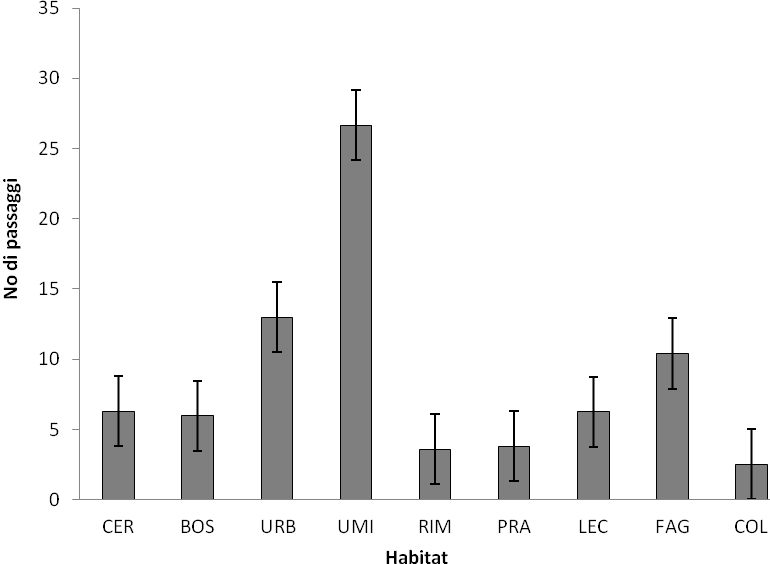
\includegraphics[width=\linewidth]{abstracts/extended_abstracts/P001_Figure1.png}
  \captionof*{figure}{Fig. 1 – Media del numero di passaggi di chirotteri per habitat. La barra di errore rappresenta gli errori standard. CER = Cerrete; BOS = Boschi misti di latifoglie; URB = Aree urbane; UMI = Aree umide; RIM = Rimboschimenti a conifere; PRA = Praterie; LEC = Querceti a leccio; FAG = Faggete; COL = Coltivi.}
\end{Figure}

\subsection*{Modelli di idoneità ambientale}
I modelli di idoneità ambientale applicati nel presente studio sono di tipo induttivo e sono basati su dati di presenza/assenza delle specie sul territorio. La progettazione dei modelli è avvenuta attraverso l’analisi dei dati raccolti sul campo e delle caratteristiche autoecologiche delle specie rilevate, che successivamente sono state correlate con variabili ambientali anche di tipo puntuale, che possono influenzare la presenza delle specie nel territorio oggetto di studio. Le variabili considerate sono: tipologia di habitat e presenza di colonie riproduttive. I modelli sono stati elaborati mediante procedure GIS (\textit{Geographic Information System}), con il \textit{software} ArcGis ver. 9.3 e utilizzando i seguenti dati geografici: la cartografia CORINE Land Cover (IV Livello, 2006) e la Carta Forestale della Basilicata. Gli habitat del parco sono stati classificati e accorpati nelle seguenti categorie: aree umide (laghi e fiumi), rimboschimenti a conifere, querceti a cerro (Cerrete), boschi misti di latifoglie (querceti, ostrieti, carpineti, etc.), coltivi, praterie, boschi di faggio (Faggete), querceti a leccio, aree urbane.

La progettazione ha previsto la restituzione di cartografie, nelle quali il diverso grado di idoneità ambientale è stato suddiviso in 4 categorie:
\begin{compactdesc}
\item[non idoneo]: ambienti che non soddisfano le esigenze ecologiche della specie;
\item[bassa idoneità]: habitat che possono supportare la presenza della specie ma in maniera non stabile nel tempo;
\item[media idoneità]: habitat che possono supportare la presenza stabile della specie, ma che nel complesso non risultano habitat ottimali;
\item[alta idoneità]: habitat ottimali per la presenza della specie.  
\end{compactdesc}
Le cartografie sono state elaborate nel sistema di riferimento UTM WGS 84 – ETRS89 fuso 33N.

\section*{Risultati e discussione}
Nel Parco Nazionale Appennino Lucano Val d’Agri Lagonegrese sono state censite ben 21 specie di chirotteri (Tab.~1, 2).

Complessivamente, mediante campionamento bioacustico sono stati rilevati 885 contatti di chirotteri (Tab.~3), e catturati 61 individui.

I risultati dell’analisi della varianza mostrano che la differenza nella media dei passaggi per gli habitat indagati è statisticamente significativa ($F_{(8,131)}$=4.70, \prob{}=0.00), per cui le tipologie ambientali hanno un effetto significativo sull’attività dei chirotteri. Le risultanze del test \textit{post hoc} di Tukey-Kramer, per un numero ineguale di unità campionarie, mostrano che l’attività differisce significativamente in 7 coppie di habitat (Tab.~4).

Le tipologie ambientali nelle quali è stata riscontrata l’attività più elevata sono le aree umide, seguite dalle aree urbane e gli habitat di tipo forestale, soprattutto le faggete; mentre gli habitat con attività decisamente più ridotta sono i rimboschimenti a conifere ed i coltivi (Fig.~1).
 
Le aree urbane, pur essendo ambienti antropizzati, hanno mostrato un’elevata attività dei chirotteri, specialmente per le specie sinantropiche. La presenza dei lampioni stradali, soprattutto nelle aree periurbane influenza positivamente l’attività ed inoltre, nel territorio del Parco, sono presenti piccoli borghi che spesso risultano strettamente connessi alle matrici naturali del paesaggio e hanno un numero elevato di edifici diroccati importanti per i chirotteri. 

Nel comprensorio del Parco e lungo i confini sono stati censiti 12 rifugi rappresentati prevalentemente da strutture di origine antropica, quali edifici in disuso e una galleria ferroviaria dismessa (Tab.~5). Gli edifici sono tutti ubicati in ambienti poco disturbati e ben integrati nella vegetazione, che nelle zone circostanti è caratterizzata da una copertura variabile da media (50\%) a elevata (80\%). Queste tipologie di rifugi sono utilizzati soprattutto nel periodo estivo e prevalentemente da Rinolofidi e individui maschi. Le colonie riproduttive sono state rilevate esclusivamente nelle cavità di origine naturale ed in particolare nel territorio di San Chirico Raparo (PZ), presso la Grotta di Sant’Angelo al Raparo, che ospita una numerosa colonia polispecifica e nel territorio di Moliterno (PZ), presso la grotta Murgia Sant’Angelo. 

\begin{figure*}[!t] %[!ht]
  \centering\small
  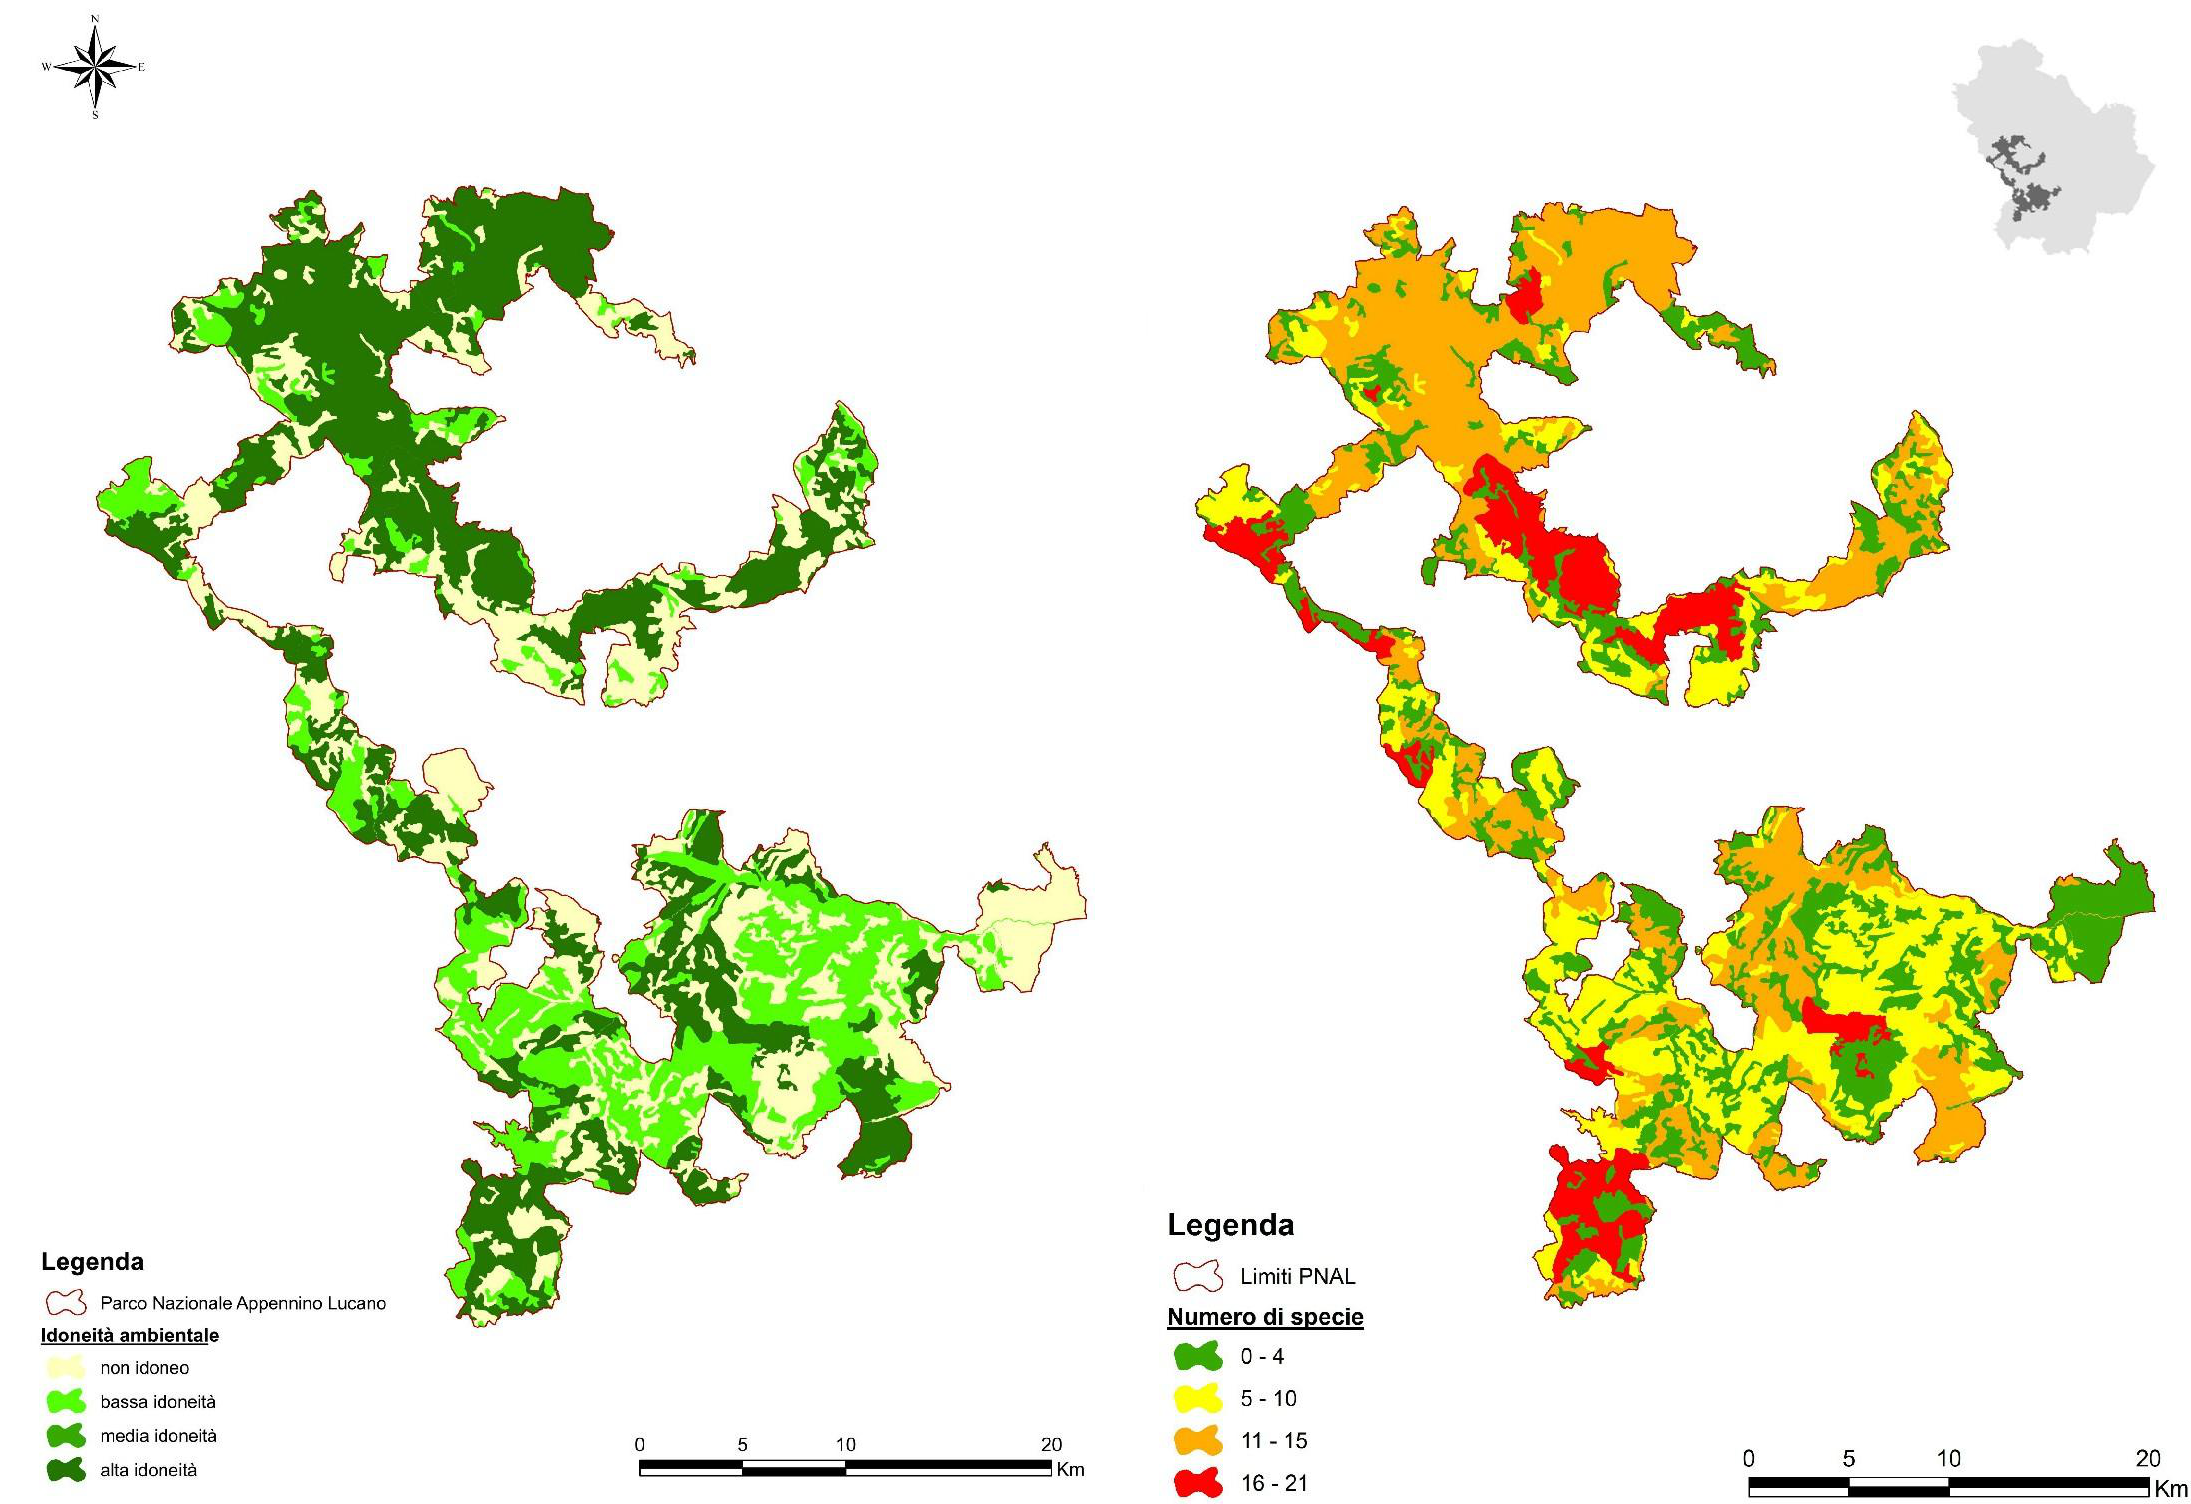
\includegraphics[width=\linewidth]{abstracts/extended_abstracts/P001_Figure2.png}
  \caption*{Fig. 2 - Mappa d’idoneità ambientale per \emph{M. bechsteinii} (a sinistra) e mappa della ricchezza in specie nel PNAL (a destra).}
\end{figure*}

\subsection*{Modelli di idoneità ambientale}
I modelli di idoneità ambientale permettono di integrare e sintetizzare le relazioni specie-ambiente e rappresentano un valido strumento di supporto alle indagini faunistiche conoscitive e ai progetti di conservazione e gestione territoriale (Duprè, 1996; Boitani et al., 2002). 

La progettazione dei modelli di idoneità ambientale ha permesso di confrontare i dati raccolti su gran parte del territorio del Parco, con i dati di letteratura, riguardanti le relazioni specie-habitat. L’analisi sul territorio si è avvalsa dei dati di cattura, relativi ai rifugi e al campionamento bioacustico. Le cartografie risultanti rappresentano la distribuzione potenziale dei chirotteri e la ricchezza di specie (S) nel territorio del Parco (Fig.~2). Gli habitat in cui è stata rilevata una maggiore ricchezza di specie (S), sono in generale gli ambienti forestali, soprattutto i boschi maturi più estesi e meno disturbati da tagli recenti, con alberi vetusti e caratterizzati dalla presenza di aree umide. Gli ambienti in grado di supportare un ridotto numero di specie sono risultati quelli maggiormente antropizzati, rappresentati dalle aree urbane, dai coltivi, soprattutto i seminativi, i rimboschimenti a conifere.

Le aree di maggior pregio per la ricchezza in specie di chirotteri sono per lo più distribuite nel settore settentrionale del Parco (M. Arioso, M. Pierfaone, Serra di Calvello, Monte Volturino, bosco di Rifreddo), dove gli ambienti forestali sono più estesi e presentano un buon grado di eterogeneità ambientale, con popolamenti di varie tipologie e classi di età. Il settore meridionale del Parco (area di Moliterno, Sarconi, San Martino d’Agri) è costituito da ambienti importanti soprattutto per la conservazione dei Rinolofidi, data la presenza di grotte con grandi colonie e di habitat elettivi per l’alimentazione. 

\section*{Conclusioni}
Le informazioni acquisite andranno ad aggiornare significativamente le conoscenze sulla diversità dei chirotteri in Italia meridionale e su scala regionale, che risultano ancora molto lacunose. Alcune specie censite sono tra le più rare nel nostro paese e in Europa, in particolare il Barbastello (\emph{Barbastella barbastellus}) e il Vespertilio di Bechstein (\emph{Myotis bechsteinii}). Importante è anche la presenza di entità criptiche, come \emph{Myotis alcathoe}, che recentemente è stato segnalato nel Parco (De Pasquale et al., 2014) e rappresenta la prima segnalazione della specie per la Basilicata. 

Gli habitat acquatici svolgono un ruolo critico per l’ecologia dei chirotteri, in quanto l’acqua può essere una risorsa limitante che condiziona la loro presenza e l’elevata densità di insetti è un fattore chiave responsabile dell’intensa attività rilevata negli habitat fluviali e lacustri (Barclay, 1991). Nel Parco, le aree umide sono ben rappresentate e molto spesso associate agli habitat forestali, in particolare la diga del Pertusillo, i laghi montani di Piana del lago, nel territorio di Marsico Nuovo (PZ) e di Laudemio, nel territorio di Lagonegro (PZ). 

Molti ambienti forestali risultano minacciati da una cattiva gestione, che ha portato ad una graduale semplificazione strutturale e compositiva dei boschi prevalentemente governati a ceduo, con una ceduazione troppo sostenuta, da turni brevi di taglio, che ha determinato una riduzione del grado di biodiversità e la perdita di rifugi principalmente rappresentati da alberi morti e vetusti.   

Tra i rifugi ipogei censiti, la grotta di Sant’Angelo al Raparo costituisce un sito di importanza biologica per la conservazione dei chirotteri, dato il numero di individui che frequentano la cavità nei diversi periodi dell’anno. Il sito risulta molto accessibile e per questo la tutela può essere compromessa dal disturbo provocato da eventuali visite a scopo didattico, turistico o speleologico, per questo sarà necessaria l’applicazione di misure di conservazione, quali ad esempio il divieto di qualsiasi forma di fruizione della cavità. 

\vskip3mm

\begin{small}
\noindent\textbf{Ringraziamenti}\\
La ricerca è stata finanziata dall’Ente Parco Nazionale dell’Appennino Lucano Val d’Agri Lagonegrese e le attività di cattura sono state autorizzate dal MATTM su parere dell’ISPRA (prot. PNM-2012-0000644). Si ringraziano tutti coloro che hanno collaborato in alcune fasi della ricerca: Dott. Antonio Conte, Sig. Andrea Giudiceandrea, Dott. Remo Bartolomei. 

\vskip3mm

\noindent\textbf{Bibliografia}\\

Agnelli P., Martinoli A., Patriarca E., Russo D., Scaravelli D., Genovesi  P., 2004. Linee Guida per il Monitoraggio dei Chirotteri. Quad. Cons. Natura, 19, Min. Ambiente – INFS

Barclay R.M.R., 1991. Population structure of temperate zone insectivorous bats in relation to foraging behaviour and energy demand. Journal of Animal Ecology 60: 165--178.

Boitani L., Falcucci A, Maiorano L., Montemaggiori A., 2002. Rete Ecologica Nazionale: il ruolo delle aree protette nella conservazione dei vertebrati. Dipartimento B.A.U., Università di Roma ``La Sapienza' , Ministero dell’Ambiente, Dir. per la Conservazione della Natura, Istituto di Ecologia Applicata, Roma.

De Pasquale P.P., Galimberti A., 2014. New records of the Alcathoe bat, \emph{Myotis alcathoe} (Vespertilionidae) for Italy, Barbastella 7, pp. XX ISSN: 1576-9720.

Dietz C., Von Helversen O., 2004. Illustrated identification key to the bats of Europe. Electronic publication, version 1.0, Tübingen, Germany.

Erkert H.G., 1982. Ecological aspects of bat activity rythms. In: Kunz T.H. (Ed.) Ecology of Bats. Plenum Press, New York. 201--242.

Fenton M.B., 1970. A  technique  for monitoring bat activity with results obtained from different environments in southern Ontario. Canadian Journal of Zoology, 48: 847--851.
 
Galimberti A., Spada M., Russo D., Mucedda M., Agnelli P., et al., 2012. Integrated Operational Taxonomic Units (IOTUs) in Echolocating bats: a bridge with Molecular  and Traditional Taxonomy. PLoS ONE  7(6): e40122. \url{doi:10.1371/journal.pone.0040122}
  
Grindal  S.D.,  Collard T.S., Brigham R.M.,  Barclay R.M., 1992. The influence of precipitation on  reproduction by  \emph{Myotis} Bats in British Columbia. American Midland Naturalist 128: 339--344.

Kramer A.C.Y., 1956). Extention of multiple range tests to group means with unequal numbers of replications. Biometrics 12: 307--310.

Kunz T.H., Kurta A., 1988. Capture methods and holding devices. In: Kunz T.H. (Ed.) Ecological and Behavioral Methods for the Study of Bats. Smithsonian Institution Press, Washington, DC. 1--29.
 
Russo D., Jones G., 2000. The two cryptic species of \emph{Pipistrellus pipistrellus} (Chiroptera: Vespertilionidae) occur in Italy: evidence from echolocation and social calls. Mammalia 64: 187--197.

Russo D., Jones G., 2002. Identification  of  twenty-two bat species  (Mammalia: Chiroptera)  from Italy by analysis  of  time-expanded  recordings  of echolocation calls. Journal of Zoology (London)  258: 91--103.
 
Tukey J.W., 1949. Comparing individual means in the analysis of variance. Biometrics 5: 99.

Whitloch M.C., Schluter D., 2010. Analisi statistica dei dati biologici. Zanichelli.

Worthington-Wilmer J., Barratt E.M., 1996. A nonlethal method of tissue sampling for genetic studies of chiropterans. Bat Research News 37: 1-–3. 

\end{small}

\end{multicols}
% % EOF % %\clearpage
% Abstract file structure example : 
% \abstitle{title here}
% \absauthors{names and superscripts for affiliations here}
% \absaddress{affiliations, starting each one with its superscripts, separate affiliations with a \break}
% \abstext{
% \index{author abbreviated name, to be placed in authors' index}
% \index{create an index entry for each author}
%  The abstract text
% }

%% Abstract title
%\abstitle{Studio sui chirotteri troglofili della Grotta di Calafarina (Pachino, SR, Sicilia sud-orientale)}

%% Author names
%\absauthors{M. \textsc{Mucedda}$^1$,  G. \textsc{Fichera}$^2$, E. \textsc{Pidinchedda}$^1$}

%\absaddress{$^1$Centro Pipistrelli Sardegna, Via G. Leopardi 1 – 07100 Sassari, Italy - batsar@tiscali.it\break
%$^2$Universität Trier Universitätsring,15 - D-54286  Trier, Germany}

%% Abstract text
%\abstext{
%%% Author names for index. State each author separately using \index{Doe J.}
%\index{Mucedda M.}
%\index{Fichera G.}
%\index{Pidinchedda E.}
%%% The actual abstract text goes here
%} %% remember to close the abstract text block brace!!
\label{ext:P001}

\loadabstr[E005]{DE PASQUALE P.P. -- La chirotterofauna dei boschi vetusti nel Parco Nazionale del Pollino}{abstracts/extended_abstracts/P005_depasquale_extended_title.tex}

\begin{multicols}{2}

\section*{Introduzione}
I boschi vetusti sono biocenosi in cui il disturbo antropico è assente o trascurabile, caratterizzate da una dinamica naturale che determina la presenza, al loro interno, di tutte le fasi di rigenerazione, compresa quella senescente con alberi di grandi dimensioni e abbondante necromassa (Blasi et al., 2010). Questi ambienti sono importanti per  le specie nemorali che beneficiano di bassi livelli di disturbo e della presenza di microhabitat (Nordén e Appelqvist, 2001), ma anche per numerose specie influenzate dalla presenza di necromassa legnosa (Christensen e Emborg, 1996), tra cui uccelli e chirotteri (Harmon et al., 1986).   

Almeno la metà delle specie di chirotteri presenti in Italia utilizza prevalentemente le foreste mature per il foraggiamento e per l’attività di \textit{roosting}. Il territorio del Parco Nazionale del Pollino è caratterizzato dalla presenza di almeno cinque formazioni forestali vetuste, che svolgono un ruolo ecologico fondamentale per numerose specie di chirotteri. Perciò è importante valutare le interazioni ecologiche tra questi mammiferi e gli habitat forestali. A tal proposito, il presente studio si pone l’obiettivo di fare un’analisi preliminare della comunità di chirotteri presente in queste biocenosi complesse, che sono potenzialmente in grado di regolarne il funzionamento.   

\section*{Materiali e metodi}
Le indagini di campo sono state condotte tra luglio ed agosto del 2015, in due boschi vetusti individuati nel versante lucano del massiccio del Pollino. I boschi sono stati censiti e caratterizzati durante il programma di ricerca finanziato dal MATTM e coordinato dall’Ente Parco Nazionale del Pollino, relativo alla costituzione della rete dei boschi vetusti nei Parchi in Italia meridionale.

Le formazioni forestali selezionate sono: il bosco misto di abete bianco (\emph{Abies alba}) e faggio (\emph{Fagus sylvatica}), il bosco misto di faggio e cerro (\emph{Quercus cerris}). Gli abieti-faggeti hanno una distribuzione piuttosto frammentaria in Italia meridionale e sono più frequenti solo nel territorio del Pollino e in Calabria (Ciancio et al., 1985). In particolare, la formazione oggetto di studio è localizzata prevalentemente nel territorio di Terranova del Pollino (PZ) ed è distribuita in una fascia altitudinale compresa tra 1350 e 1550 m s.l.m.; è costituita da 3 nuclei a bosco vetusto, compresi parzialmente nel bosco di Cugno dell’Acero e nel SIC IT9210075 ``Lago Duglia, Casino Toscano''. La cerreta-faggeta è presente nel territorio di San Severino lucano (PZ) e il nucleo a bosco vetusto è collocato nella fascia altitudinale compresa tra 700 e 900 m s.l.m.. La formazione forestale è denominata ``Bosco Magnano'' ed è compresa interamente nel SIC IT9210040 omonimo.

Il protocollo di ricerca ha previsto indagini mediante rilievi ultrasonori e catture temporanee in entrambe le tipologie forestali. I rilievi ultrasonori sono stati effettuati mediante un \textit{bat detector} in espansione temporale (10$\times$), modello Pettersson D240X. I campioni sono stati registrati mediante un registratore digitale Edirol R-09, con frequenza di campionamento a 44.1~kHz e risoluzione a 16~bit. L’attività dei chirotteri è stata quantificata rilevando il numero di passaggi di chirotteri per tipologia forestale attraverso il conteggio delle sequenze dei segnali di ecolocalizzazione (Fenton, 1970).

L’ordine di campionamento è stato effettuato in modo \textit{random} e in 15 punti d’ascolto per ogni tipologia di bosco; i punti sono stati selezionati anche nelle aree forestali a medesima consociazione limitrofe ai nuclei a bosco vetusto (Fig.~1) e il tempo di campionamento è stato di 15 minuti per punto, a partire da 30 minuti dopo il tramonto. L’attività dei chirotteri può essere influenzata dall’ora della notte e da fattori ambientali, come vento, pioggia, umidità, temperatura (Avery, 1985; Rydell, 1993; Vaughan et al., 1997; O’Donnell, 2000), per cui i rilievi ultrasonori sono stati effettuati nelle prime 4 ore della notte, fase in cui l’attività è più elevata e, solo durante le notti con temperature > a 10 °C, senza precipitazioni e vento. 

\subsection*{Catture temporanee}
La cattura è una tecnica di campionamento utilizzata soprattutto nei casi in cui si desidera identificare le specie, l’età, il sesso e lo stato riproduttivo dei chirotteri. Durante le operazioni di cattura sono state utilizzate due reti per sito, identiche, per lo stesso tempo di campionamento (Barlow, 1999). Le reti, del tipo \textit{mistnet} (Ecotone), rispettivamente di 6.0$\times$2.50~m e 12.0$\times$2.50~m, entrambe con dimensione di maglia 14~mm (lunghezza di un lato della maglia), sono state posizionate lungo l’asse dei torrenti, in prossimità di stagni e lungo corridoi forestali, per un tempo di campionamento di 3 ore, a partire da 30 minuti dopo il tramonto.

Il successo di cattura diminuisce quando un sito è campionato per più notti consecutive (Kunz e Brock, 1975), per cui i pipistrelli sono stati catturati in 3 siti diversi per ogni tipologia forestale ed i campionamenti non sono stati ripetuti nello stesso sito.
 
Gli individui catturati sono stati pesati mediante bilancia digitale con precisione $\pm$0.1~g, misurati mediante un calibro digitale autobloccante, con precisione $\pm$0.1~mm; per ogni individuo è stato  identificato il sesso, la classe di età (adulti e giovani), lo stato riproduttivo. I giovani sono stati identificati attraverso l’osservazione dell’ossificazione incompleta tra le epifisi e le diafisi delle ossa metacarpali e delle falangi (Antony, 1988). Per l’identificazione morfologica sono state consultate le chiavi analitiche di Dietz e von Helversen (2004). Gli individui identificati come appartenenti a specie criptiche (\emph{Myotis mystacinus} \textit{group}), sono stati sottoposti a una biopsia della pelle (\textit{biopsy punch}); il materiale biologico è stato estratto mediante un \textit{punch} avente 3~mm di diametro, direttamente dalla membrana caudale (uropatagio) e conservato in provette con etanolo assoluto e in frigorifero (Worthington-Wilmer et al., 1996). I campioni sono stati analizzati mediante il metodo del DNA Barcoding (Hebert et al., 2003; Galimberti et al., 2012) e identificati geneticamente presso lo ZooPlantLab del Dipartimento di Biotecnologie e Bioscienze dell’Università degli Studi di Milano-Bicocca.

Le specie criptiche \emph{P. pipistrellus} e \emph{P. pygmaeus} sono state identificate misurando la frequenza di massima energia dei segnali di ecolocalizzazione emessi durante l’attività di foraggiamento e al rilascio dopo la cattura (Russo e Jones, 2000), per mezzo del \textit{software} BatSound v. 3.3 (Pettersson elektronik AB, Uppsala, Sweden).

\subsection*{Analisi dei dati}
L’effetto dell’habitat, sull’attività dei chirotteri, è stato valutato tramite il test U di Mann-Whitney a una coda, per verificare se l’attività differisce in modo statisticamente significativo tra cerreta-faggeta e abetina-faggeta. 

Successivamente, si è ipotizzato che la distribuzione del sesso e delle classi di età non è casuale, ma che esiste un certo effetto dovuto al tipologia forestale e all’altitudine, per cui le differenze nella distribuzione dei sessi e delle classi di età dei pipistrelli catturati tra tipologie forestali, sono state testate mediante l’utilizzo del test $\chi^2$, con due categorie. L’analisi è stata effettuata su tre trattamenti: \Male{} adulti, \Female{} adulte e giovani. 

Le analisi statistiche sono state effettuate per mezzo del \textit{software} Minitab 17, con un livello di significatività p=0.05.

Per confrontare lo sforzo di campionamento per tipologia forestale, è stato utilizzato un indice di cattura (numero di individui catturati, per m\textsuperscript{2} di \textit{mistnet}, per ore di campionamento), (Hodgkison et al. 2004; Kunz et al. 2009).


\begin{table*}[t]
\caption*{Tab. 1 - Specie catturate, media e deviazione standard (DS) della lunghezza avambraccio (AV) e lunghezza del quinto dito (LD-V) in mm, numero di individui per sesso e classi di età.}
%\label{tab:table1}
\centering\small
\begin{tabular}{lccccc}
\textbf{Specie}&\textbf{AV}&\textbf{LD-V}&\textbf{\Male{} Adulti} & \textbf{\Female{} Adulte} & \textbf{Giovani}\\
\hline
\emph{M. daubentonii} & (36.99$\pm$0.69) & (44.78$\pm$0.98) & 6 & 3 & 0\\
\emph{M. mystacinus} & (35.14$\pm$0.36) & (43.16$\pm$0.69) & 3 & 1 & 0\\
\emph{M. alcathoe} & (32.94$\pm$0.36) & (40.15$\pm$0.61) & 1 & 2 & 3\\
\emph{M. nattereri} & (38.07$\pm$0.20) & (47.12$\pm$0.43) & 1 & 0 & 1\\
\emph{M. bechsteinii} & (41.02$\pm$1.39) & (51.62$\pm$1.38) & 1 & 2 & 1\\
\emph{M. emarginatus} & (38.92) & (50.06) & 0 & 0 & 1\\
\emph{M. myotis} & (61.62$\pm$2.35) & (76.30$\pm$1.27) & 4 & 0 & 1\\
\emph{P. auritus} & (38.19$\pm$0.40) & (48.56$\pm$0.50) & 0 & 1 & 2\\
\emph{B. barbastellus} & (41.52) & (51.22) & 0 & 1 & 0\\
\emph{N. leisleri} & (42.44$\pm$0.45) & (44.91$\pm$0.97) & 9 & 0 & 0\\
\emph{E. serotinus} & (53.74) & (62.65) & 1 & 0 & 0\\
\emph{H. savii} & (33.50$\pm$1.32) & (40.16$\pm$0.67) & 2 & 1 & 0\\
\emph{P. pipistrellus} & (30.22$\pm$0.78) & (37.51$\pm$1.38) & 1 & 6 & 6\\
\emph{P. pygmaeus} & (29.72$\pm$0.72) & (34.39$\pm$0.59) & 1 & 1 & 1\\
\end{tabular}
\end{table*}

\section*{Risultati}
Durante le indagini di campo sono stati rilevati 213 passaggi di chirotteri, per un totale di 24 ore di campionamento, in entrambe le tipologie forestali. L’attività è risultata più elevata nella cerreta-faggeta, rispetto all’abetina-faggeta e la differenza è statisticamente significativa (U=54, \prob{}=0.0079, Mann-Whitney U-test).
 
Sono stati catturati 64 individui in 18 ore di campionamento (Tab.~1). Nella cerreta-faggeta sono stati catturati 48 individui appartenenti a 12 specie: \emph{M. mystacinus} (N=2), \emph{M. alcathoe} (N=6), \emph{M. daubentonii} (N=9), \emph{M. nattereri} (N=2), \emph{M. enarginatus} (N=1), \emph{P. auritus} (N=1), \emph{B. barbastellus} (N=1), \emph{N. leisleri} (N=8), \emph{E. serotinus} (N=1), \emph{P. pipistrellus} (N=12), \emph{P. pygmaeus} (N=2), \emph{H. savii} (N=3).
 
Nell’abetina-faggeta sono stati catturati 16 individui appartenenti a 7 specie: \emph{M. myotis} (N=5), \emph{M. bechsteinii} (N=4), \emph{M. mystacinus} (N=2), \emph{P. auritus} (N=2), \emph{N. leisleri} (N=1), \emph{P. pipistrellus} (N=1), \emph{P. pygmaeus} (N=1).

\begin{Figure} %[!ht]
  \centering\small
  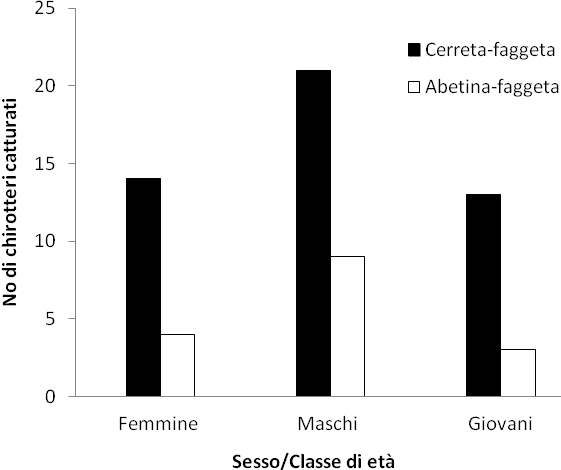
\includegraphics[width=\linewidth]{abstracts/extended_abstracts/P005_Figure1.png}
  \captionof*{figure}{Fig. 1 –  Distribuzione del sesso e delle classi di età (femmine adulte, maschi adulti e giovani) nei chirotteri catturati, per tipologia forestale. Le differenze sono tutte statisticamente significative.}
\end{Figure}


I pipistrelli per ambo sessi e classi di età sono stati catturati in numero significativo nella cerreta-faggeta, rispetto all’abetina-faggeta (femmine adulte: $\chi^2$=5.55, g.d.l.=1, \prob{}-value=0.018; maschi adulti: $\chi^2$=4.80, g.d.l.=1, \prob{}-value=0.028; giovani: $\chi^2$=6.25, g.d.l.=1, \prob{}-value=0.012), (Fig.~1). Le femmine adulte non sono state catturate in numero significativo rispetto ai maschi adulti nella cerreta-faggeta ($\chi^2$=1.40, g.d.l.=1, \prob{}-value=0.237) e nell’abetina-faggeta ($\chi^2$=1.92, g.d.l.=1, \prob{}-value=0.166). Gli adulti, rispetto ai giovani sono stati catturati in numero significativo nella cerreta-faggeta ($\chi^2$=10.08, g.d.l.=1, \prob{}-value=0.001) e nell’abetina-faggeta ($\chi^2$=6.25, g.d.l.=1, \prob{}-value=0.012).

L’indice di cattura calcolato per la cerreta-faggeta è 0.039, mentre per l’abetina-faggeta è 0.013.

\section*{Discussione}
I dati mostrano che il tipo di bosco, la sua struttura e l’altitudine sono in grado di influenzare l’attività dei chirotteri. Inoltre, anche la disponibilità di prede è un fattore che potrebbe favorire l’attività, sebbene nel presente studio non sia stato considerato.

La cerreta-faggeta ha una più elevata ricchezza di specie e dei livelli di attività, a causa sia dell’altitudine, sia dell’eterogeneità strutturale che caratterizza il popolamento. 

Il bosco, specialmente nelle aree più interne è costituito da diversi microhabitat e ha una struttura disetanea, con abbondante necromassa (alberi morti in piedi, rami e alberi caduti a terra) e potenziali \textit{roost} (Fig.~2).    

\begin{Figure}
  \centering\small
  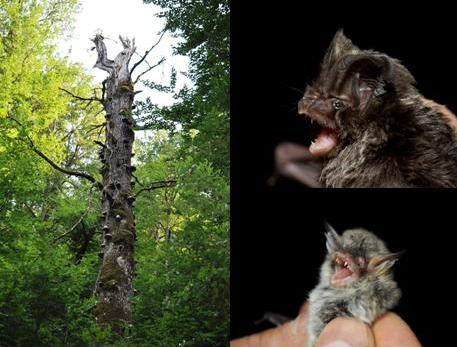
\includegraphics[width=\linewidth]{abstracts/extended_abstracts/P005_Figure2.png}
  \captionof*{figure}{Fig. 2 –  Cerro (\emph{Quercus cerris}) morto in piedi a Bosco Magnano (a sinistra). \emph{Barbastella barbastellus} (in alto, a destra), foto: Antonio Conte. \emph{Myotis nattereri} (in basso, a destra), foto: Serena Di Santo.}
\end{Figure}

Un altro fattore che influenza positivamente l’attività e la disponibilità di insetti è dato dalla presenza del Torrente Peschiera, che attraversa gran parte dell’area forestale. Questa eterogeneità ambientale favorisce la presenza di chirotteri che cacciano sulla volta forestale (es. \emph{N. leisleri}), nello spazio aereo all’interno della foresta e lungo i margini (es. \emph{P. pipistrellus}, \emph{P. pygmaeus}), tra la vegetazione (\emph{P. auritus}, \emph{B. barbastellus}, \emph{M. nattereri}), sulla superficie dell’acqua (\emph{M. daubentonii}). A tal proposito l’uso differenziale dello spazio di foraggiamento, per specie che vivono nella stessa area forestale, può determinare una stratificazione verticale dell’attività in habitat complessi (Francis, 1994; Kalcounis et al., 1999; Hayes et al., 2000). 

L’altitudine e altri fattori geografici possono influenzare anche la distribuzione dei sessi, infatti, le femmine adulte generalmente utilizzano le foreste presenti più a bassa quota, per minimizzare i costi di termoregolazione e incrementare l’efficienza di foraggiamento (Cryan et al., 2000). Le femmine adulte sono state catturate con maggiore frequenza nella cerreta-faggeta, e anche i maschi, sebbene nei mesi estivi tendano a disperdersi fino alle quote elevate, sono stati catturati più frequentemente nella stessa tipologia di bosco. 

Il numero di individui giovani e di femmine adulte catturate tende a eguagliarsi in entrambe le tipologie di bosco e questo fenomeno, per quanto concerne il bosco presente più a bassa quota (cerreta-faggeta), può essere dovuto sia a vantaggi legati alla maggiore disponibilità di prede, sia al mantenimento dei contatti materni (Grindal et al., 1999).

L’indagine svolta rappresenta il primo studio sulla chirotterofauna del Parco Nazionale del Pollino e ha permesso di censire specie rare e di pregio naturalistico e conservazionistico, che rappresentano una componente faunistica importante per gli ecosistemi forestali e sono potenzialmente in grado di influenzare l’organizzazione delle biocenosi (\textit{keystone species}), attraverso il controllo dell’abbondanza di insetti. Importanti sono anche gli habitat oggetto di studio, che pur avendo una limitata estensione, possono contenere risorse chiave (\textit{keystone resources}), come le cavità degli alberi (Cockle et al., 2011) che sono cruciali ai fini della sopravvivenza dei chirotteri e di molte altre specie. 

La ricerca ha permesso anche di indagare la chirotterofauna associata alle faggete degli Appennini con \emph{Abies alba}, che sono un habitat prioritario (cod. 9220$\ast$) per la conservazione, ai sensi della direttiva 92/42/CE. Queste consociazioni sono piuttosto rare in Italia e nella parte meridionale della penisola hanno subito notevoli alterazioni, dovute all’attività antropica fin dall’epoca romana (Susmel, 1959; Ciancio et al., 1985).    

Le informazioni acquisite sono di carattere preliminare, in quanto solo delle indagini pluriannuali possono delineare i \textit{trend} sul grado di frequentazione dell’area di studio, le fluttuazioni dei livelli di attività e le variazioni della ricchezza in specie. A tale proposito assumono particolare importanza le indagini pluriannuali condotte attraverso stime numeriche delle colonie di chirotteri e la valutazione degli indici di attività per valutare gli impatti antropici a breve e a lungo termine, su ecosistemi e biodiversità (Kunz et al., 2009).

I dati circa la fedeltà dei pipistrelli a specifici siti di foraggiamento e di \textit{roosting} all’interno delle aree forestali e l’uso preferenziale di differenti tipologie di boschi, dominati dalla presenza di determinate specie arboree, sebbene siano molto limitati in Italia (Russo et.al. 2004, 2010) possono fornire informazioni utili per la gestione degli habitat e del paesaggio forestale.

Come si evince dal Piano AIB 2012--2014 predisposto dal PN del Pollino, l’Ente si impegna a proporre la promozione e l’attuazione di una gestione forestale sostenibile anche attraverso le attività di formazione per gli operatori del settore. Per questo sarebbe opportuno considerare una gestione forestale orientata alla conservazione, all’incremento dei pipistrelli e dei loro rifugi, sviluppando delle linee guida dettagliate da inserire nei programmi di formazione per le ditte agricolo-forestali e per i tecnici degli Enti locali. 

\vskip3mm

\begin{small}
\noindent\textbf{Ringraziamenti}\\
La ricerca è stata realizzata grazie a un finanziamento dell’Ente Parco Nazionale del Pollino e del MATTM. Le attività di cattura sono state autorizzate dal MATTM su parere dell’ISPRA (prot. PNM-2014-0003894). Si ringrazia sentitamente il Dott. For.le Aldo Schettino (Ente Parco Nazionale del Pollino), l’Isp. Lorenzo Viceconte e l’Agente Gioiadonato (Corpo Forestale dello Stato). 

\vskip3mm

\noindent\textbf{Bibliografia}\\

Anthony E.L.P., 1988. Age determination in bats. In: Kunz T.H. (Ed.) Ecological and Behavioral Methods for the Study of Bats. Smithsonian Institution Press, Washington, DC. 47--58.

Barlow K.E., 1999. Expedition Field Techniques. Bats. The Expedition Advisory Centre, Royal Geographical Society, London.

Blasi C., Burrascano S., Maturani A., Sabatini F.M., 2010. Foreste Vetuste in Italia, Contributo Tematico alla Strategia Nazionale per la Biodiversità. Ministero dell’Ambiente e della Tutela del Territorio e del Mare.

Christensen M., Emborg J., 1996. Biodiversity in natural versus managed forests. Forest Ecology and Management 85: 47--51.

Ciancio O., Iovino F., Menguzzato G., Mirabella A., 1985. L’Abete (\emph{Abies alba} Mill.) in Calabria: possibilità e limiti di diffusione e ridiffusione. Annali Ist. Sper. Selvicoltura, vol. 16: 7--249.

Cockle K.L., Martin K., Wesolowski T., 2011. Woodpeckers, decay, and the future of cavity-nesting vertebrate communities worldwide. Frontiers in Ecology and Conservation 9: 377--382.

Cryan P.M., Bogan M.A., Altenbach J.S., 2000. Effect of elevation on distribution of female bats in the Black Hills, South Dakota. Journal of Mammalogy 81: 719--725.

Dietz C., Von Helversen O., 2004. Illustrated identification key to the bats of Europe. Electronic publication, version 1.0, Tübingen, Germany.

Ente Parco Nazionale del Pollino, 2012. Piano delle Attività di Previsione, Prevenzione e Lotta Attiva contro gli Incendi Boschivi, periodo di validità 2012--2014, redatto dai funzionari: Valicenti A., De Vivo G., Schettino A.

Erkert H.G., 1982. Ecological aspects of bat activity rythms. In: Kunz T.H. (Ed.) Ecology of Bats. Plenum Press, New York. 201--242.

Fenton M.B., 1970. A  technique  for monitoring bat activity with results obtained from different environments in southern Ontario. Canadian Journal of Zoology 48: 847--851;.

Francis C.M., 1994. Vertical stratification of fruit bats (Pteropodidae) in lowland dipterocarp rainforest in Malaysia. Journal of Tropical Ecology 10: 523--530.

Galimberti A., Spada M., Russo D., Mucedda M., Agnelli P., et al., 2012. Integrated Operational Taxonomic Units (IOTUs) in Echolocating bats: a bridge with Molecular  and Traditional Taxonomy. PLoS ONE  7(6): e40122. \url{doi:10.1371/journal.pone.0040122}
  
Grindal S.D., Morrissette J.l., Brigham R.M., 1999. Concentration of bat activity in riparian habitats over an elevational gradient. Canadian Journal of Zoology 77: 972--977.

Harmon M.E., Franklin J.F., Swanson F.J., Sollins P., Gregory S.V., Lattin J.D., Anderson N.H., Cline S.P., Aumen N.G., Sedell J.R., Lienkaemper G.W., Cromack K. Jr., Cummins K.W., 1986. Ecology of coarse woody debris in temperate ecosystems. Advances in Ecological  Researchs 15: 133

Hayes J.P., Gruver J.C., 2000. Vertical stratification of bat activity in an old-growth forest in western Washington. Northwest Science 74: 102--108.

Kalcounis M.C., Hobson K.A., Brigham R.M., Hecker K.R., 1999. Bat activity in the boreal forest: importance of stand type and vertical strata. Journal of Mammalogy 80: 673--682.

Kunz T.H., Brock C.E., 1975. A comparison of mist nets and ultrasonic detectors for monitoring flight activity of bats. Journal of Mammalogy 58: 309--315.

Kunz T.H., Parsons S., 2009. Ecological and Behavioral Methods for the Study of Bats, 2\textsuperscript{nd} Editiln. The Johns Hopkins University Press.

Nòrden B., Appelqvist T., 2001. Conceptual problems of ecological continuity and its bioindicators. Biodiversity and Conservation 10: 779--791.

O'Donnell C.F.J., 2000. Influence of season, habitat, temperature and invertebrate availability of nocturnal activity of the New Zealand long-tailed bat (\emph{Chalinolobus tuberculatus}). N.Z.J. Zool. 27: 207--221.

Russo D., Jones G., 2000. The two cryptic species of \emph{Pipistrellus pipistrellus} (Chiroptera: Vespertilionidae) occur in Italy: evidence from echolocation and social calls. Mammalia 64: 187--197;.

Russo D., Cistrone L., Jones G., et al., 2004. Roost selection by Barbastelle bats (\emph{Barbastella barbastellus}, Chiroptera: Vespertilionidae) in beech woodlands of central Italy: consequences for conservation. Biol. Conserv. 117: 73--81.

Russo D., Cistrone L., Garonna A.P., Jones G., 2010. Reconsidering the importance of harvested forests for the conservation of tree-dwelling bats. Biodivers. Conserv. 19: 2501--2515.

Whitloch M.C., Schluter D., 2010. Analisi statistica dei dati biologici. Zanichelli.

Worthington-Wilmer J., Barratt E.M., 1996. A nonlethal method of tissue sampling for genetic studies of chiropterans. Bat Research News 37: 1-–3.

\end{small}

\end{multicols}
% % EOF % %\clearpage
% Abstract file structure example : 
% \abstitle{title here}
% \absauthors{names and superscripts for affiliations here}
% \absaddress{affiliations, starting each one with its superscripts, separate affiliations with a \break}
% \abstext{
% \index{author abbreviated name, to be placed in authors' index}
% \index{create an index entry for each author}
%  The abstract text
% }

%% Abstract title
%\abstitle{Studio sui chirotteri troglofili della Grotta di Calafarina (Pachino, SR, Sicilia sud-orientale)}

%% Author names
%\absauthors{M. \textsc{Mucedda}$^1$,  G. \textsc{Fichera}$^2$, E. \textsc{Pidinchedda}$^1$}

%\absaddress{$^1$Centro Pipistrelli Sardegna, Via G. Leopardi 1 – 07100 Sassari, Italy - batsar@tiscali.it\break
%$^2$Universität Trier Universitätsring,15 - D-54286  Trier, Germany}

%% Abstract text
%\abstext{
%%% Author names for index. State each author separately using \index{Doe J.}
%\index{Mucedda M.}
%\index{Fichera G.}
%\index{Pidinchedda E.}
%%% The actual abstract text goes here
%} %% remember to close the abstract text block brace!!

\loadabstr[E018]{MUCEDDA M., FICHERA G., PIDINCHEDDA E. -- Studio sui chirotteri troglofili della Grotta di Calafarina (Pachino, SR, Sicilia sud-orientale)}{abstracts/extended_abstracts/C018_mucedda.ea_extended_title.tex}

\begin{multicols}{2}

\section*{Introduzione}
La Grotta di Calafarina, accatastata come SR 7011, è una cavità naturale situata nel comune di Pachino, che ospita nel suo interno una grande colonia di pipistrelli, che la rendono una delle più importanti della Sicilia.

Nel corso del biennio 2004--2005 è stato effettuato uno studio, con controlli periodici della popolazione di chirotteri all’interno della grotta, che è stato ripetuto nel triennio 2011-2013, allo scopo di stabilire quali specie siano presenti, accertarne l’entità numerica e ricostruire il loro ciclo biologico annuale. Brevi note sull’attività svolta nella prima fase compaiono in Mucedda \& Bertelli (2009).


\section*{Materiali e metodi}
Le visite di controllo all’interno della grotta sono state effettuate utilizzando materiali e attrezzature speleologiche. Per la documentazione fotografica sono state utilizzate macchine fotografiche digitali reflex Canon EOS 300D e 600D, con flash elettronici Canon Speedlite 550 EX e Metz 44. Il conteggio fotografico dei pipistrelli è stato realizzato al computer con un programma di grafica in modo preciso o comunque con un margine di errore estremamente ridotto.

Le catture dei pipistrelli ove necessario sono state realizzate con l’uso di retino e canna telescopica da 9 metri.

Le misurazioni biometriche degli animali sono state effettuate con un calibro della precisione di 0.1 mm e una pesola della precisione di 0.5 g.

Tutti gli esemplari sono stati prontamente liberati al termine delle operazioni. 

Le registrazioni dei suoni dei pipistrelli sono state effettuate con due Bat-detector Pettersson D980 e D240x, in modalità \textit{Time expansion}, più un registratore Zoom H2. Le elaborazioni al computer sono state realizzate con il programma Batsound della Pettersson.

Le temperature sono state misurate con un termometro digitale della precisione di 0.1\degree{}~C.

Per l'identificazione di \emph{Rhinolophus mehelyi} sono stati utilizzati i caratteri morfologici di Mucedda et al. (2009), mentre per \emph{Myotis myotis}/\emph{blythii} è stata usata la formula discriminante di Arlettaz (1995).

Tutte le fasi dello studio sono state realizzate seguendo le norme delle ``Linee guida per il monitoraggio dei Chirotteri'' (Agnelli et Al., 2004). 

Le attività sono state condotte con le autorizzazioni dell’Assessorato Regionale Territorio e Ambiente della Regione Sicilia (1814 del 26/05/2004 e 1742 del 01/06/2012) e del Ministero dell’Ambiente e della tutela del Territorio e del Mare (DPN/2D/2004/7489 del 15/03/2004 e 0009358 del 07/06/2012).

\subsection*{La grotta}
La Grotta di Calafarina è una cavità di origine carsica, situata lungo la zona costiera a sud di Marzamemi, nella estrema punta meridionale della Sicilia, che si apre con una piccola dolina di crollo a 15 m di quota, su una formazione calcarea miocenica di Calciruditi dell'Aquitaniano (Colacicchi, 1963). 

\begin{Figure} %[!ht]
  \centering\small
  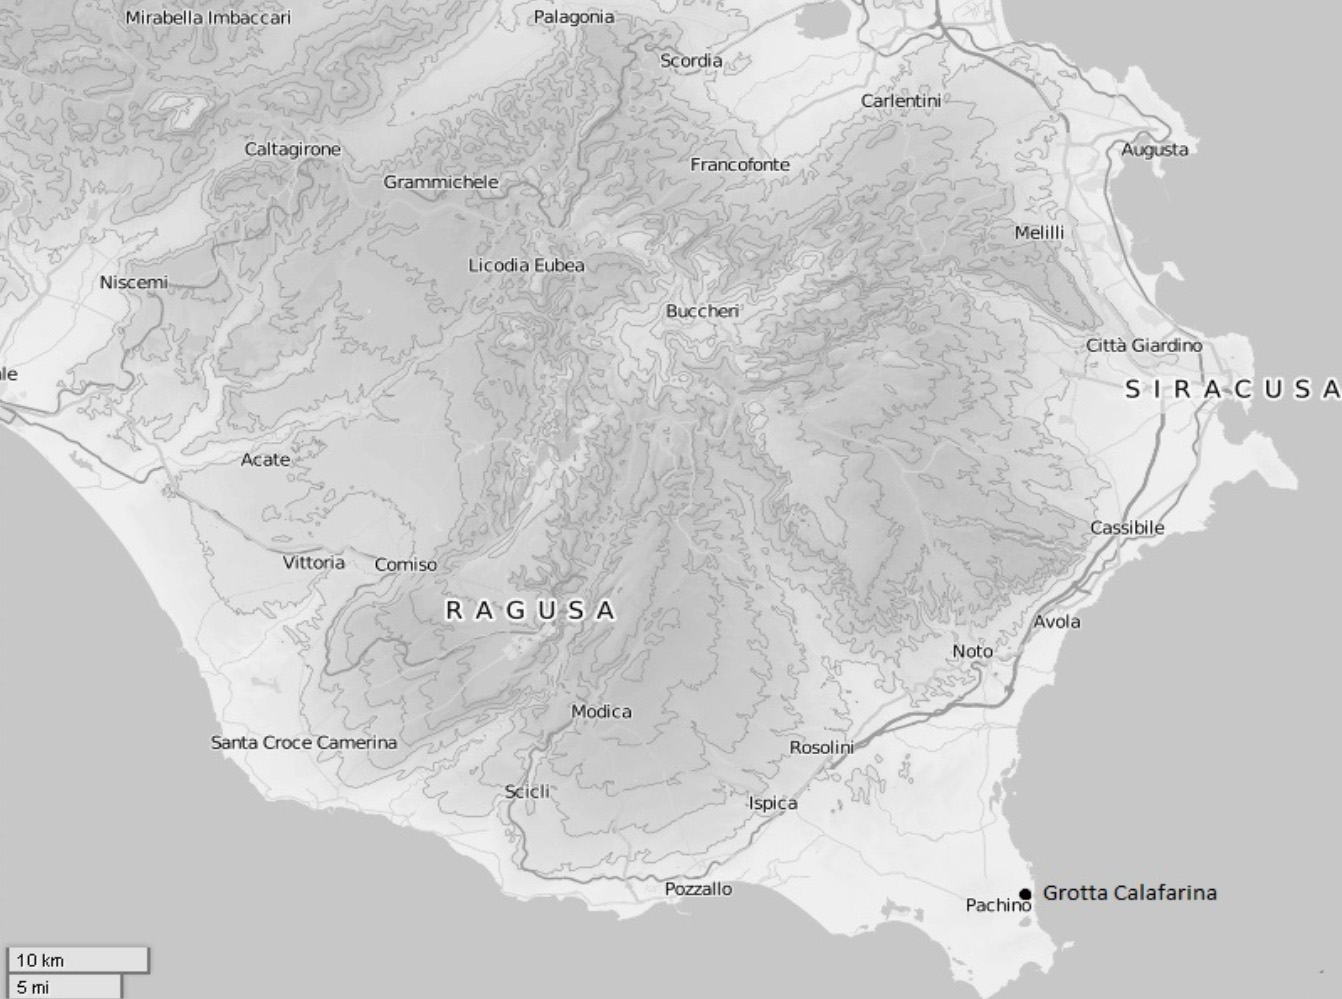
\includegraphics[width=\linewidth]{abstracts/extended_abstracts/C018_Figure1.png}
  \captionof*{}{Fig. 1 – Posizione geografica della Grotta di Calafarina.}
\end{Figure}
\begin{figure*}[t] %[!ht]
  \centering\small
  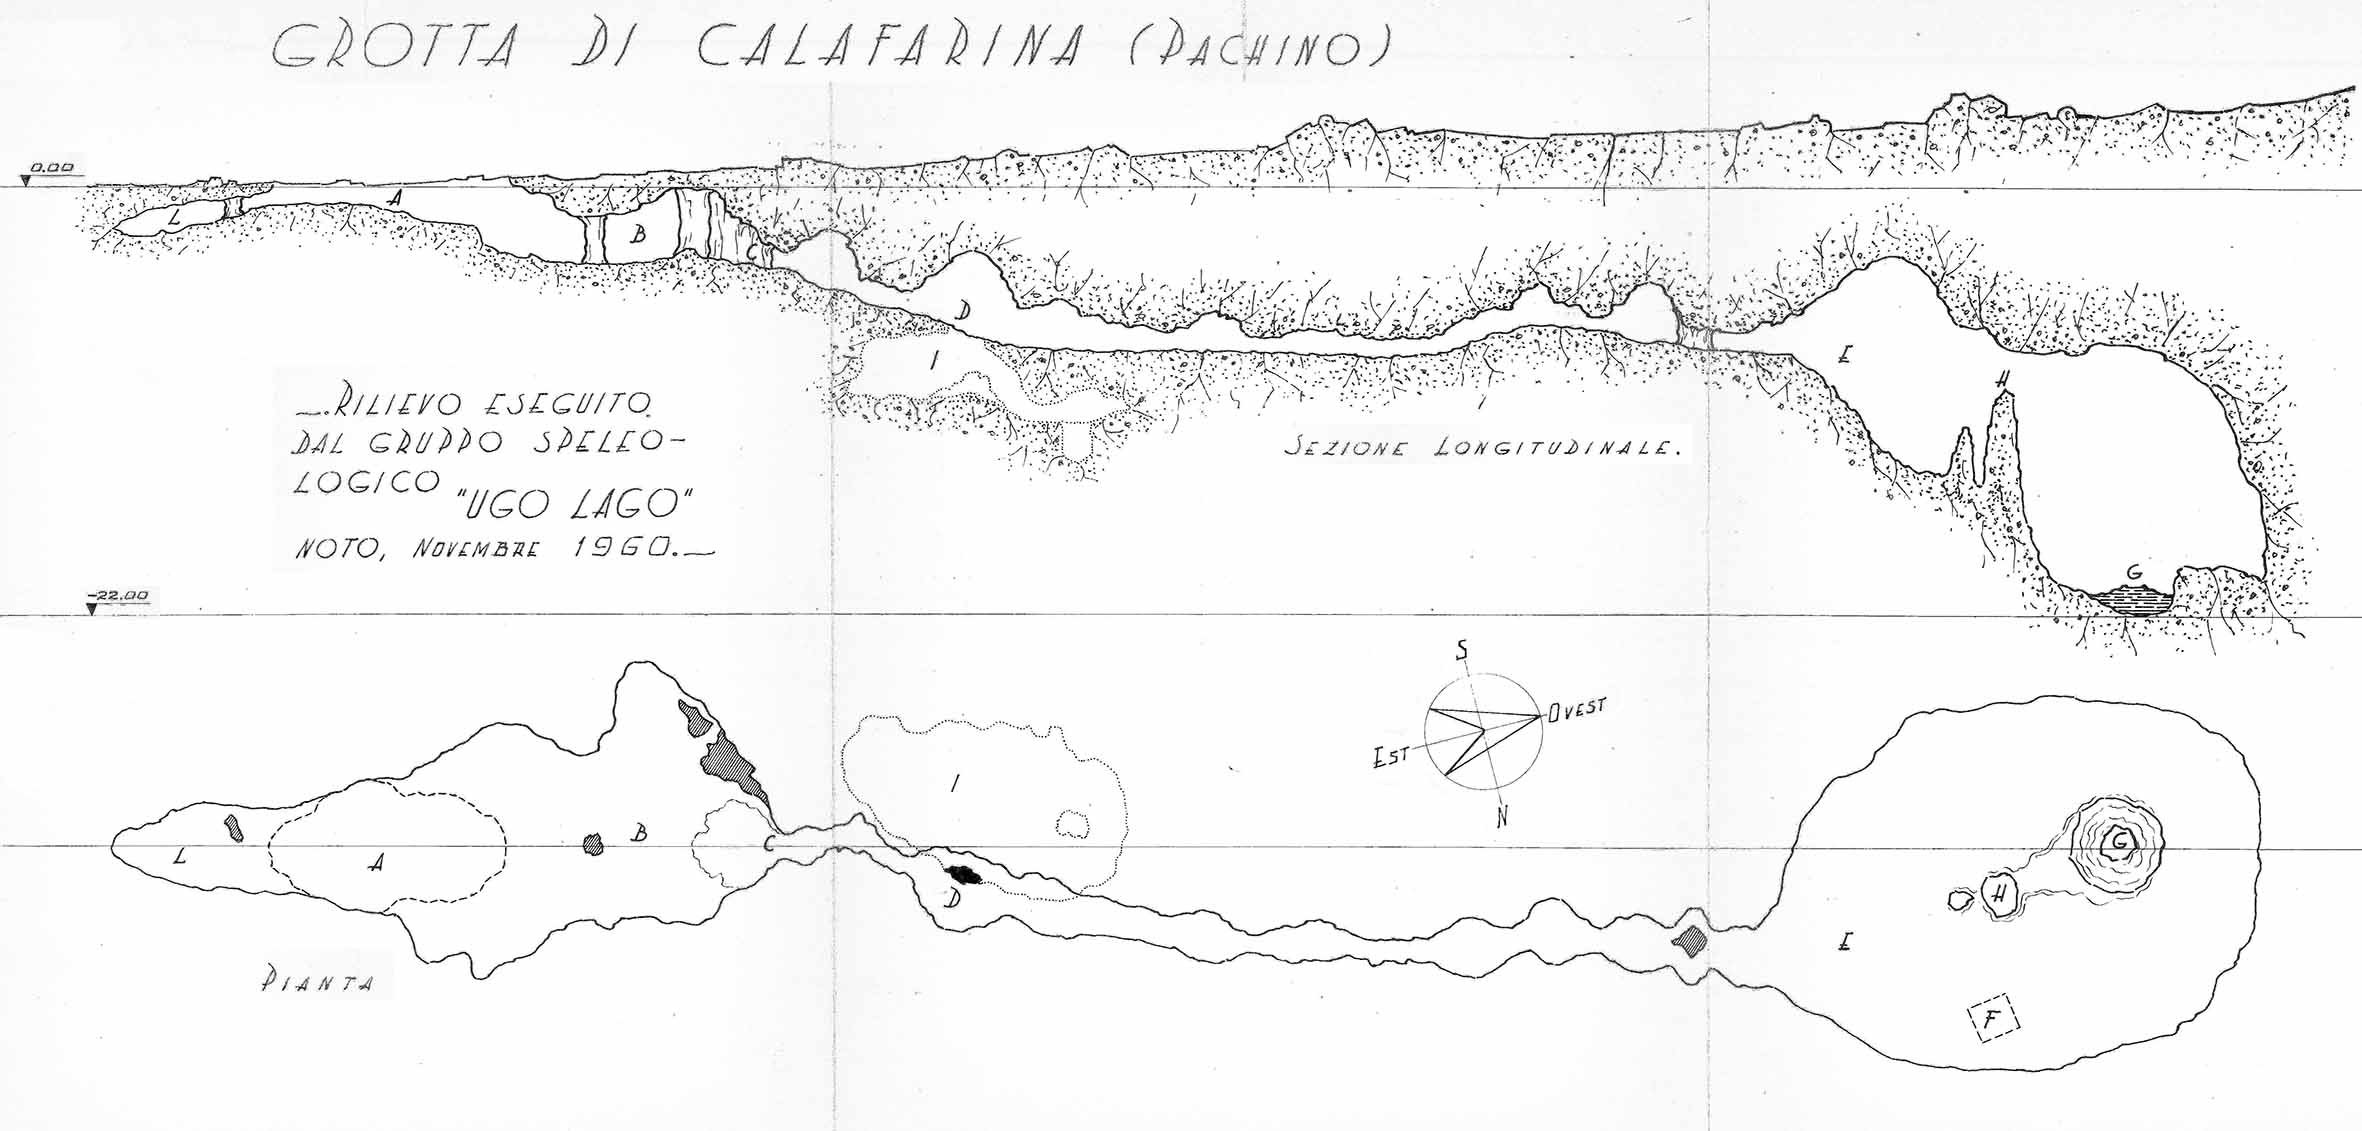
\includegraphics[width=\linewidth]{abstracts/extended_abstracts/C018_Figure2.png}
  \caption*{Fig. 2 – Rilievo topografico della grotta (Gruppo Speleologico ``Ugo Lago'').}
\end{figure*}

La cavità dopo l’ingresso presenta una salto verticale di circa 3 m e poi si sviluppa ad andamento sub orizzontale, con un disagevole cunicolo di circa 40 m che sbuca in un’ampia sala terminale discendente (la ``Camera dei Pipistrelli'' di Ragonese), di circa 20$\times$30 m, dove si stabilisce una grande colonia di pipistrelli. Sul lato destro della sala si innalza verso l’alto uno stretto pozzo artificiale di 10 m che proviene dalla superficie, che risulta essere attualmente occluso, ma che negli anni '60 risultava aperto e in parte rischiarava la sala (Ragonese, 1968). La grotta ha uno sviluppo orizzontale di 123 m e un dislivello di -22 m. La sua posizione è data dalle seguenti coordinate: Lat.  \ang{36;43;18.45}~N – Long. \ang{15;07;02.14}~E (WGS84 da GoogleEarth).

\begin{figure*}[t] %[!ht]
  \centering\small
  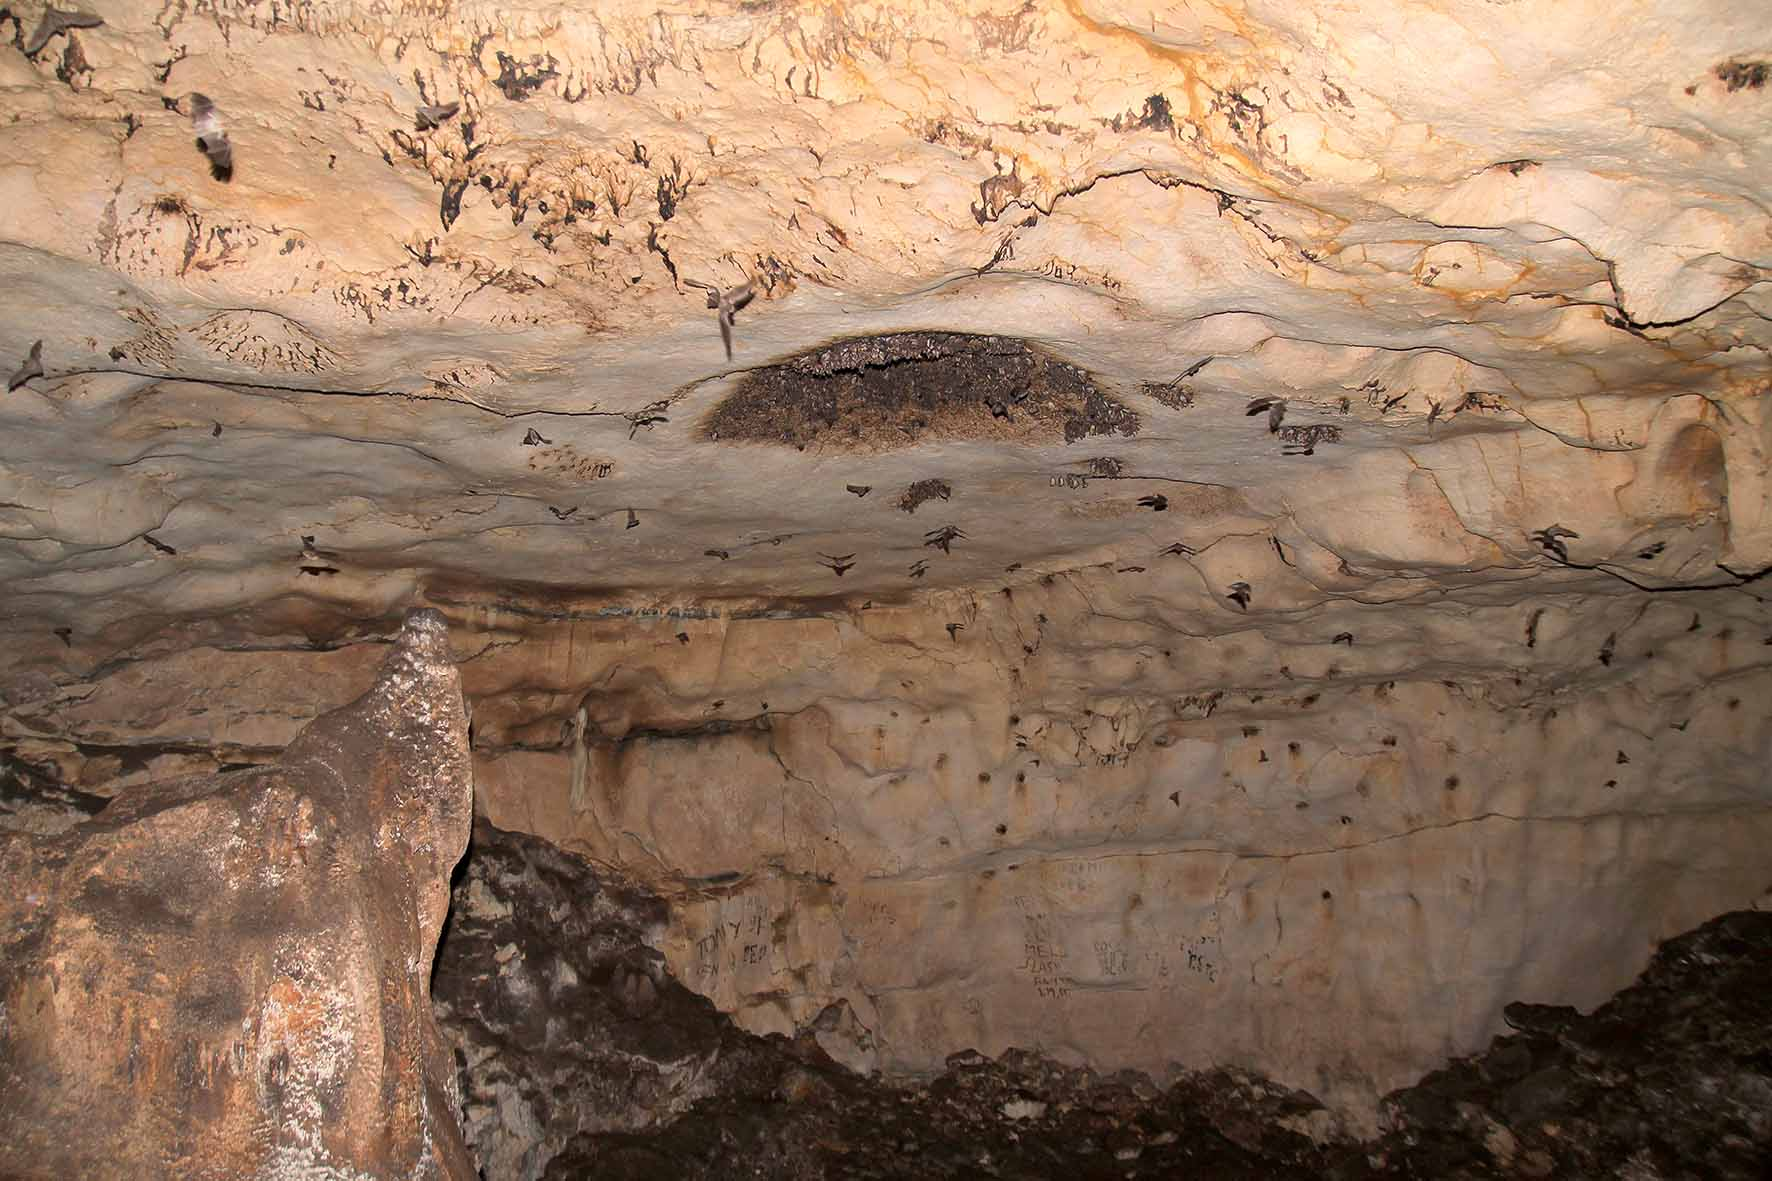
\includegraphics[width=\linewidth]{abstracts/extended_abstracts/C018_Figure3.png}
  \caption*{Fig. 3 - Veduta della sala terminale (Foto Gaetano Fichera).}
\end{figure*}

\subsection*{Note bibliografiche}
Il primo a darci notizia della presenza di pipistrelli nella Grotta di Calafarina è Orsi (1907), che descrive la cavità come ricchissima di guano e riferisce che l’ingresso della cavità, prima molto angusto, era stato allargato con l'utilizzo di mine.

La popolazione chirotterologica viene studiata per la prima volta da Ragonese (1967), del Gruppo Speleologico ``Ugo Lago'  di Noto, che la sceglie dal 1961 come stazione di inanellamento per i pipistrelli. Ragonese riferisce che la colonia è costituita da \emph{Rhinolophus ferrumequinum}, \emph{Myotis myotis} e \emph{Myotis capaccinii}, che arrivano a migliaia in aprile e maggio, le femmine partoriscono in estate e ripartono a settembre, asserendo che è un mistero dove essi vadano, mentre d'inverno c'è solo una decina di esemplari in semiletargo. Nel 1968 Ragonese pubblica un intero libro dal titolo ``Nel buio della Calafarina'' dedicato alla cavità in tutti i suoi aspetti descrittivi, archeologici e faunistici, confermando quanto già detto prima sui pipistrelli. Dice di aver inanellato 518 individui dal 9/7/1961 al 9/7/1967, la maggior parte dei quali sono \emph{M. myotis} (452), con pochi \emph{M. capaccinii} (61) e qualche  \emph{R. ferrumequinum} (5), riportando i dati in una lunga tabella.

\begin{figure*}[t] %[!ht]
  \centering\small
  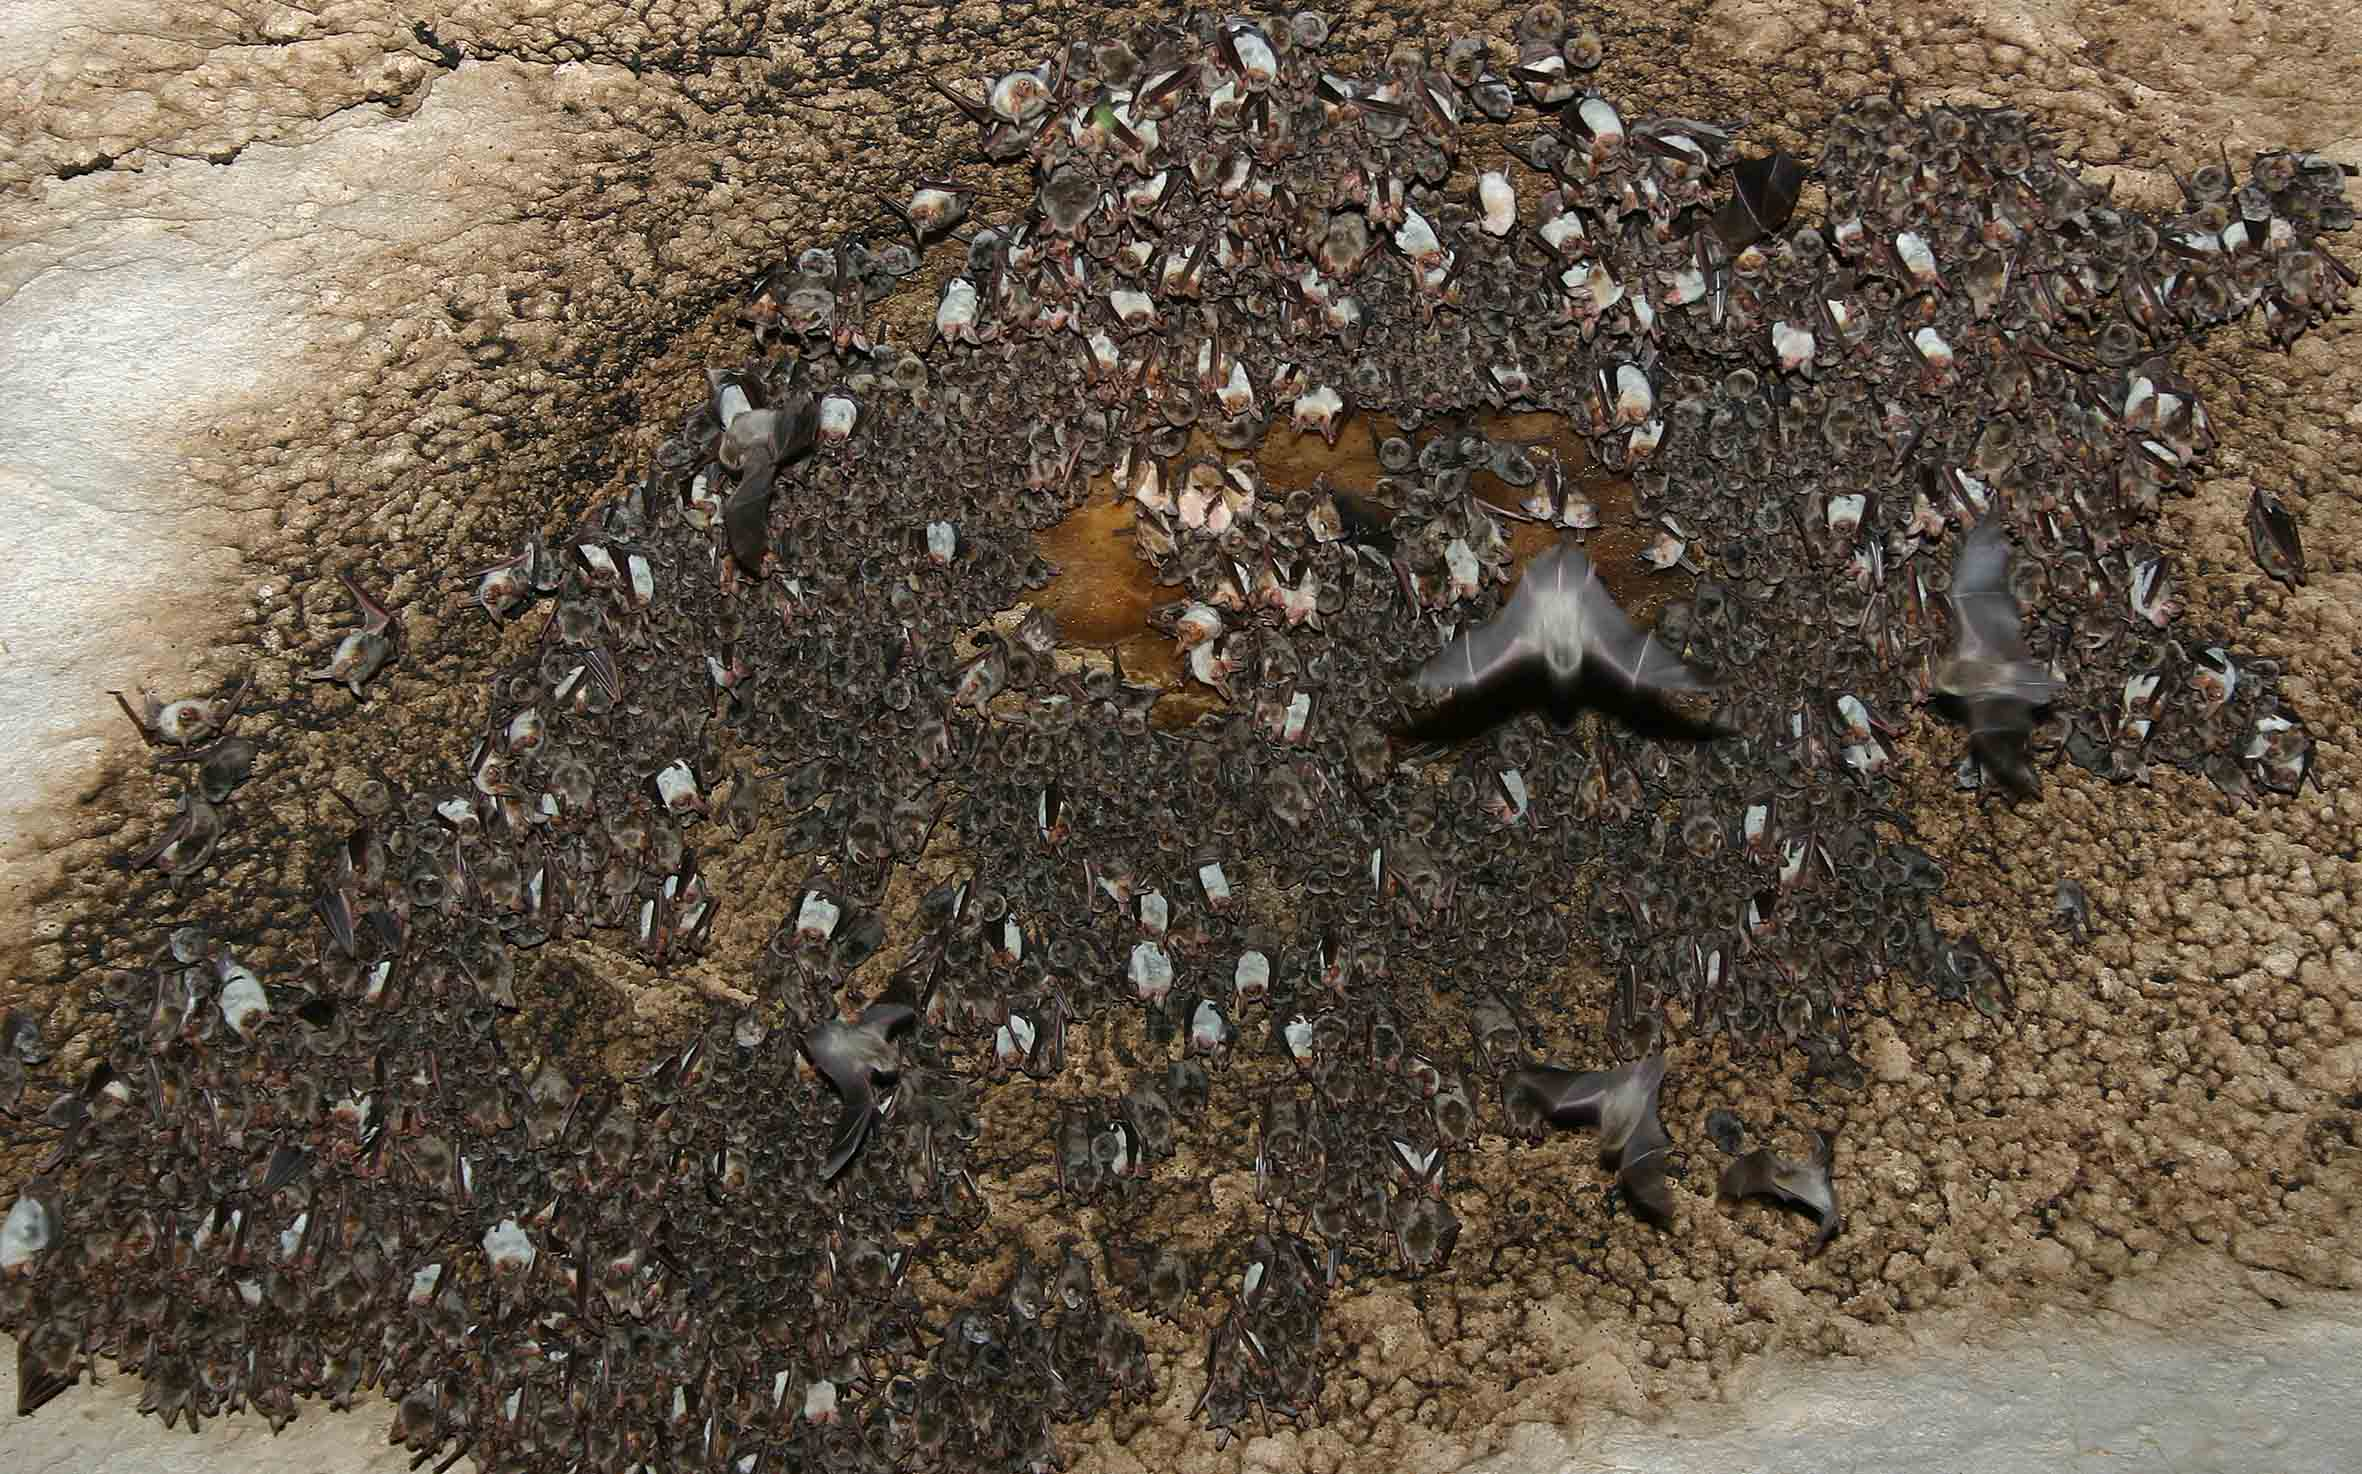
\includegraphics[width=\linewidth]{abstracts/extended_abstracts/C018_Figure4.png}
  \caption*{Fig. 4 – La colonia di pipistrelli nel mese di agosto (Foto Mauro Mucedda).}
\end{figure*}

Ragonese, con i suoi collaboratori, è stato probabilmente l’unico a studiare di persona i pipistrelli di Calafarina e pubblicare dati originali. I successivi autori infatti si limitano a citare i suoi lavori e i suoi dati, senza apparentemente aggiungere nulla di nuovo. Così Caruso (1978), Caruso e Costa (1978), Zava et Al. (1986), Caruso (1995), Caruso e Grasso (1996) per la grotta riportano tutti \emph{M. myotis}, \emph{M. capaccinii} e \emph{R. ferrumequinum}. Ragonese \& Contoli (1996) stranamente citano invece solo \emph{M. myotis} e \emph{M. capaccinii}.

Infine Mucedda et al. 2009 citano \emph{M. myotis}, \emph{M. capaccinii}, \emph{R. mehelyi} e \emph{M. schreibersii}, aggiungendo quindi le ultime due specie che sino ad allora non erano note per la cavità.

\section*{Risultati} 
Il nostro studio ha consentito di accertare nella grotta la presenza di 5 specie di chirotteri:
\begin{compactitem}
\item Rinolofo maggiore (\emph{Rhinolophus ferrumequinum} Schreber, 1774)
\item Rinolofo di Mehely (\emph{Rhinolophus mehelyi} Matschie, 1903)
\item Vespertilio maggiore (\emph{Myotis myotis} Borkhausen 1797)
\item Vespertilio di Capaccini (\emph{Myotis capaccinii} Bonaparte,1837)
\item Miniottero (\emph{Miniopterus schreibersii} Kuhl, 1817)
\end{compactitem}

I pipistrelli si radunano stagionalmente nell’ampia sala terminale, dove formano una grande colonia plurispecifica, che si aggrega principalmente in un nicchione del soffitto nella parte inferiore, e anche in gruppi minori in altre zone della sala. In altre parti della grotta sono stati osservati solo rari e occasionali esemplari. 

Numericamente la colonia risulta formata in massima parte da \emph{M. myotis} e da \emph{M. schreibersii}, che sono le specie preponderanti, e da un numero molto ridotto di \emph{M. capaccinii} e di \emph{R. mehelyi}. Il \emph{R. ferrumequinum} è stato osservato invece in pochi esemplari solamente in una occasione nel cunicolo che porta alla sala interna e quindi non si aggrega alle altre specie che formano la colonia.

La maggior parte dei pipistrelli non utilizza la grotta tutto l’anno, ma essi compiono dei movimenti migratori che li portano nella cavità generalmente in primavera, per poi gradualmente abbandonarla in autunno.

Qui di seguito riportiamo le osservazioni relative al ciclo annuale, con la dinamica della popolazione chirotterologica, nelle sue variazioni stagionali.

A causa della sua elevata temperatura interna, la Grotta di Calafarina non è idonea per il letargo, e pertanto in periodo invernale (dicembre-gennaio) sono presenti solo 30--40 esemplari tra \emph{M. schreibersii}, \emph{M. myotis} e \emph{M. capaccinii}. Già in febbraio si registra un lieve incremento nel numero di animali presenti nella Grotta, che possono arrivare a circa 200 esemplari.

In primavera la popolazione cresce notevolmente, con l’arrivo delle colonie migratorie dei pipistrelli, il cui numero in aprile raggiunge i 1300 esemplari e in maggio arriva a 1800, in gran parte \emph{M. myotis} e \emph{M. schreibersii}, con pochi \emph{M. capaccinii} e pochissimi \emph{R. mehelyi}; queste due ultime specie sono difficili da quantificare dato il loro esiguo numero rispetto alle due specie preponderanti. In questo periodo nel cunicolo di accesso alla sala terminale sono stati osservati anche alcuni \emph{R. ferrumequinum}, che costituiscono una presenza solo sporadica e occasionale nella grotta. Nel mese di maggio avvengono le prime nascite.

Nei mesi estivi la colonia cresce numericamente a seguito delle nascite, con oltre 2000 esemplari stimati, che rimane invariata in genere sino a settembre. E’ stata osservata la presenza di neonati di tutte e quattro le specie M. myotis, M. schreibersii, M. capaccinii e R. mehelyi.
Con l’arrivo dell’autunno si riscontra un calo numerico dei pipistrelli, che pian piano abbandonano la grotta diretti alle località di svernamento, riducendosi in novembre a qualche centinaio di esemplari. 

Nel corso del monitoraggio, a causa dei pipistrelli subito in movimento e le conseguenti difficoltà, il numero dei pipistrelli è stato spesso stimato. Solo in alcune occasioni nella colonia si sono potuti eseguire conteggi fotografici esatti degli animali, con i seguenti risultati:
\begin{compactitem}
\item 27 agosto 2004: 506 \emph{M. myotis}, 810 \emph{M. schreibersii}, 19 \emph{R. mehelyi} e 28 \emph{M. capaccinii}.
\item 27 aprile 2005: 570 \emph{M. myotis}, 820 \emph{M. schreibersii}, 4 \emph{R. mehelyi}.
\item 6 maggio 2013: 789 \emph{M. myotis}, 1082 \emph{M. schreibersii}, 6 \emph{R. mehelyi}.
\end{compactitem}

Come già detto, la Grotta di Calafarina è una cavità molto calda. Le temperature misurate nella Sala dei Pipistrelli infatti oscillano nel corso dell’anno tra 21\celsius{} e 22\celsius{}, che data l’elevata umidità degli ambienti sotterranei rendono la presenza dell’uomo all’interno particolarmente problematica. È incredibile come a queste temperature sia possibile riscontrare pipistrelli in letargo, anche se solo poche decine di esemplari.

Il Rinolofo di Mehely è stato oggetto anche di un’indagine bioacustica, basata sulla registrazione dei suoni di un limitato numero di esemplari, tenendo gli animali fermi in mano a una distanza di 30 cm dal microfono del Bat detector, come indicato in Russo et al. (2007). Gli individui di \emph{R. mehelyi} da noi analizzati in Sicilia mostrano una frequenza media dei segnali emessi più alta di quelli della Sardegna. Gli esemplari sardi infatti hanno registrato valori di 104.3--109.8 kHz di frequenza, mentre i pochi campioni esaminati di Calafarina hanno registrato valori di 111.4--113.2 kHz. L’argomento meriterebbe ulteriori indagini di approfondimento.

\section*{Discussione}
Il monitoraggio ha consentito di stabilire che la Grotta di Calafarina è un sito di riproduzione, con la presenza di una colonia \textit{nursery} composta da 4 specie di pipistrelli: \emph{Miniopterus schreibersii}, \emph{Myotis myotis}, \emph{Myotis capaccini} e \emph{Rhinolophus mehelyi}, con la preponderanza numerica delle prime due.

Questo tipo di aggregazione mista è molto frequente per i chirotteri troglofili in ambiente cavernicolo, riscontrata spesso in Sardegna (Mucedda et al., 1995), in Corsica (Courtois et al., 2011) e in Sicilia (Mucedda et al., in stampa), sia con tutte e quattro le specie insieme che con sole tre di esse.

Il \emph{Rhinolophus ferrumequinum} è invece occasionale e non si riproduce in questa cavità, in quanto, come è noto questa specie nel periodo estivo abbandona le grotte e preferisce utilizzare rifugi quali edifici, cavità artificiali più asciutte e altre tipologie di strutture.

La colonia riproduttiva della Grotta Calafarina è una delle più importanti della Sicilia e geograficamente risulta essere allo stato attuale la più meridionale d'Italia. In Sicilia orientale per entità numerica è seconda solo alla Grotta dei Pipistrelli di Pantalica, dove in estate si aggregano sino a 4000 chirotteri (Mucedda et al., in stampa).

Le nascite hanno inizio nella prima decade del mese di maggio con i primi parti di \emph{Myotis capaccinii} e \emph{Myotis myotis}. I \emph{Miniopterus schreibersii} partoriscono invece poco più tardi a fine maggio e in giugno. I \emph{Rhinolophus mehelyi} partoriscono per ultimi in giugno.

Terminato il periodo riproduttivo, ha inizio la fase degli accoppiamenti e in agosto e in settembre sono state osservate coppie di \emph{Myotis myotis}, isolate dalla colonia principale.

Non sono emerse variazioni di rilievo tra le osservazioni del 2004--2005 e quelle del 2011--2013, per cui si ritiene che a distanza di 7--8 anni la popolazione di chirotteri della Grotta di Calafarina sia al momento stabile e quindi non soffra di particolari pressioni.

Tra le specie di pipistrelli che utilizzano la grotta, possiamo considerare il \emph{Rhinolophus mehelyi} come quello più rilevante dal punto di vista protezionistico. La sua presenza è particolarmente importante perché in tutta la Sicilia sono note attualmente due sole stazioni per questa specie e quella di Calafarina risulta essere sino ad oggi l’unica colonia riproduttiva attualmente nota nella regione (Mucedda et al. 2009). 

Il Rinolofo di Mehely si aggrega con le altre specie nella colonia, ma è numericamente molto ridotto. Nel corso dei monitoraggi, nel periodo estivo sono stati osservati tra un minimo di 7 e un massimo di 20 esemplari. È presente anche in autunno, ma in periodo invernale risulta invece assente. Si tratta pertanto di una specie particolarmente minacciata, in posizione talmente critica da poterla definire ``quasi in via di estinzione'' per la Sicilia.

\subsection*{Confronti con il passato}
È interessante notare che la colonia di pipistrelli è passata indenne nel tempo a grandi rimaneggiamenti che hanno interessato la Grotta di Calafarina, quali l’allargamento dell’ingresso con le mine, lo scavo del pozzo artificiale nella sala terminale e i lavori di estrazione del guano. È questo proprio un caso di adattamento da parte dei chirotteri, che sino ai giorni nostri continuano ad utilizzare la cavità come rifugio, nonostante le azioni di pesante disturbo succedutesi nel tempo.

Osservando i dati storici, la tipologia dei movimenti migratori stagionali da noi riscontrati nella grotta appare analoga a quanto osservato negli anni ’60 da Ragonese (1967, 1968).

Differenze sostanziali risultano invece riguardo alle specie presenti. Ragonese infatti parla di una colonia formata da soli \emph{R. ferrumequinum}, \emph{M. myotis} e \emph{M. capaccinii}, mentre attualmente risultano presenti anche \emph{R. mehelyi} e \emph{M. schreibersii} che prima non erano stati riscontrati. Sulla base di queste considerazioni, si potrebbero ipotizzare due possibilità: Ragonese potrebbe aver commesso un errore nella identificazione e potrebbero essere sfuggite queste due ultime specie, oppure più probabilmente nell’arco di 50 anni la popolazione di chirotteri ha subito delle modificazioni sostanziali. Poichè lo stesso Ragonese (1968) dichiara che all’epoca il pozzo interno che sbuca in superficie era aperto, si potrebbe pensare che la chiusura di tale pozzo (che non si sa quando sia avvenuta) abbia modificato le caratteristiche climatiche della grotta (circolazione d’aria, umidità e temperatura), e si siano create condizioni più idonee alle due specie \emph{R. mehelyi} e \emph{M. schreibersii} che hanno così iniziato a frequentare la grotta. 

Appare comunque strano che \emph{R. ferrumequinum} risultasse presente in passato nella colonia estiva, perché come già detto questa specie in estate è solita trasferirsi in altri rifugi quali edifici e cavità artificiali.

Come già visto in precedenza, Ragonese aveva inanellato nell’arco di 6 anni 452 \emph{M. myotis}, 61 \emph{M. capaccinii} e 5 \emph{R. ferrumequinum}, per un totale di 518 individui. Andando ad esaminare i dati in modo più approfondito, risulta che i \emph{M. myotis} erano 225 femmine, 214 maschi e 13 indeterminati, i \emph{M. capaccinii} 49 femmine e 12 maschi e i \emph{R. ferrumequinum} 1 femmina, 3 maschi e 1 indeterminato. Benchè non sia possibile conoscere la situazione della totalità degli animali presenti, si evidenzia che la colonia di riproduzione non era costituita da sole femmine (54.6\% delle catture), ma il numero dei maschi presenti era sempre notevole (45.4\% delle catture). L’inanellamento di soli 5 \emph{R. ferrumequinum} sembrerebbe confermare che questa specie non fosse numerosa ma solo occasionale. Esaminando i dati pubblicati, risulta che nell’arco dei 6 anni di attività si sono registrate solo 3 ricatture. Questo fa pensare che la colonia possa aver risentito delle attività di inanellamento e molti pipistrelli nel tempo abbiano probabilmente preferito non ritornare nella grotta.

Poco si può ipotizzare sugli spostamenti migratori. Sino ad oggi non sono note in Sicilia colonie di letargo invernale di \emph{Myotis myotis}, se non rifugi di pochi esemplari, per cui rimangono sconosciute le località in cui si trasferisce questa specie. Per \emph{M. schreibersii} e \emph{M. capaccini} sono invece note delle colonie invernali sull’Etna (Fichera et al., in stampa), per cui è probabile ritenere che essi possano trascorrere il letargo proprio sull’Etna. 

L’identificazione dei \emph{M. myotis} è stata effettuata su un numero ridotto di esemplari, basandosi sulle misurazioni biometriche di avambraccio e orecchio col metodo di Arlettaz (1995). Nella gran moltitudine di pipistrelli della colonia non possiamo comunque escludere la presenza anche di esemplari di \emph{M. blythii}, che spesso forma colonie miste col \emph{M. myotis}, e questa problematica richiederebbe un approfondimento. Sinora comunque non risultano note in Sicilia colonie di riproduzione con entrambe le specie.

\subsection*{L’estrazione del guano}
Orsi (1907) riferisce che la Grotta di Calafarina era ricchissima di guano, che veniva estratto dal proprietario, il Marchese Antonio Di Rudinì, utilizzandolo per fertilizzare le proprie terre. Ragonese (1968) ritiene che il pozzo artificiale che si innalza nella sala terminale era stato forse scavato dal Marchese, proprio per l’estrazione del guano. La presenza di grandi depositi di guano è la testimonianza della frequentazione da parte dei chirotteri da tempi molto lontani. Non si hanno però informazioni dettagliate sulle quantità estratte e sul periodo esatto in cui abbia avuto luogo l’attività estrattiva. 

Un’altro riferimento bibliografico su questo tema è quello di Paris (1899), che cita analisi di guano proveniente da Pachino, riferibile molto probabilmente alla Grotta di Calafarina. 

\subsection*{Interventi di tutela}
Data l’importanza della popolazione di pipistrelli della Grotta di Calafarina, le cui specie sono tutte inserite in Allegato II della Direttiva Habitat, sarebbero auspicabili degli interventi di tutela, almeno per evitare che persone incontrollate accedano alla sala terminale, arrecando grave disturbo alla colonia. 

Il sito è infatti privo di protezioni e pertanto potenzialmente minacciato, data la sua facilità di accesso e notorietà presso la popolazione locale. Sarebbe necessario sensibilizzare gli abitanti del luogo, con attività divulgative e cartellonistica appropriata.

Si deve segnalare che qualora, per malaugurata ipotesi, qualcuno dovesse riaprire l’imbocco del pozzo esterno posto nella sala terminale, si avrebbero delle gravi modificazioni nelle caratteristiche ambientali della grotta, con rischio elevato di perdita della colonia di pipistrelli.

Non è facile prevedere un intervento di tutela della grotta, perché la cavità è molto conosciuta e frequentata dalla gente del posto, soprattutto i ragazzi di Pachino e Portopalo.

Per un intervento attivo di tutela, occorre tenere presente che non è possibile l’installazione di un cancello a totale chiusura dell’ingresso della grotta, perché i Miniotteri non sono in grado di passare attraverso le sbarre, come è già successo nella Grotta Palombara di Melilli (Mucedda et al., in stampa). Anziché un cancello si potrebbe prevedere una recinzione alta intorno all’imbocco, ma si deve segnalare che una recinzione installata in passato era già stata abbattuta.

\vskip3mm

\begin{small}
\noindent\textbf{Ringraziamenti}\\
Si ringraziano il Centro Speleologico Etneo, Rosario Ardilio, Maria Luisa Bertelli, Mariacristina Borrello, Federica Calabrese, Dalma Cultrera, Sergio Firinu, Iolanda Galletti, Tiziana Grech, Domenico Longo, Fabio Morreale, Michele Nanzarelli, Alfio Nicolosi, Giorgio Sabella che hanno partecipato alle attività o ci hanno fornito utili informazioni per le indagini.

\vskip3mm

\noindent\textbf{Bibliografia}\\

Agnelli P., Martinoli A., Patriarca E., Russo D., Scaravelli D., Genovesi P. (Eds.), 2004. Linee guida per il monitoraggio dei Chirotteri: indicazioni metodologiche per lo studio e la conservazione dei pipistrelli in Italia. Quad. Cons. Natura 19, Min. Ambiente-Ist. Naz. Fauna Selvatica.

Arlettaz R., 1995. \emph{Myotis myotis} – \emph{Myotis blythii}. Ecology of the sibling mouse-eared bats, Horus Publishers Martigny, Switzerland, 44--52.

Caruso D., 1978. Il popolamento cavernicolo della Sicilia (Ricerche faunistiche ed ecologiche sulle grotte di Sicilia. VII). Lav. Soc. Ital. Biogeogr. Nuova serie, Vol. VII (Pubblicato 1982): 587--614. 

Caruso D., 1995. L’attuale stato delle conoscenze sulla fauna delle grotte di Sicilia (Ricerche faunistiche ed ecologiche sulla grotte di Sicilia. VIII). Atti I Convegno Regionale di Speleologia della Sicilia, Ragusa 1990, Vol. II: 349--378.

Caruso D., Costa G., 1978. Ricerche faunistiche ed ecologiche sulle grotte di Sicilia. VI – Fauna cavernicola di Sicilia (Catalogo ragionato). Animalia, Catania, 5 (1--3): 423-513.

Caruso D., Grasso R., 1996. La fauna delle grotte. Atti Convegno ` La fauna degli Iblei' , Noto, 1995: 201--281.

Colacicchi R., 1963. Geologia del territorio di Pachino (Sicilia meridionale). Geologia romana, II, 1963, pp. 343--404.

Courtois J.Y., Rist D., Beuneux G., 2011. Les chauves-souris de Corse. Albiana, Ajaccio: pp. 167.

Fichera G., Mucedda M., Pidinchedda E., Catalano P. Sperlinga G., (in stampa). Aggiornamento delle conoscenze sulla chirotterofauna del comprensorio etneo (Sicilia orientale). In: Madonia G., Panzica La Manna M., Vattano M. (Eds.) Atti del 5\degree{} Congresso Regionale di Speleologia della Sicilia, 23--24 novembre 2013, Castello di Rampinzeri, Santa Ninfa (TP).

Mucedda M., Castorina R., Fichera G., Pidinchedda E., (in stampa). Osservazioni sui pipistrelli di due importanti grotte degli Iblei: la Grotta Palombara (Melilli) e la Grotta di Pantalica (Sortino) (Sicilia orientale). In: Madonia G., Panzica La Manna M., Vattano M. (Eds.) Atti del 5\degree{} Congresso Regionale di Speleologia della Sicilia, 23--24 novembre 2013, Castello di Rampinzeri, Santa Ninfa (TP).

Mucedda M., Pidinchedda, Bertelli M. L., 2009. Status del Rinolofo di Mehely (\emph{Rhinolophus mehelyi}) (Chiroptera, Rhinolophidae) in Italia. Atti del 2\degree{} Convegno Italiano sui Chirotteri, Serra San Quirico (AN), 21--23 novembre 2008: 89--98.

Mucedda M., Bertelli M.L., 2009. Cronache sulle ricerche di pipistrelli in Sicilia nel 2004 e 2005. Bollettino del Gruppo Speleologico  Sassarese, n. 19, 19--27.

Mucedda M., Murittu G., Oppes A., Pidinchedda E., 1995. Osservazioni sui Chirotteri troglofili della Sardegna. Boll. Soc. Sarda Sci. Nat., 30: 97--129.

Orsi P., 1907. La grotta di Calafarina presso Pachino (Siracusa), abitazione e sepolcro. Bullettino di Paletnologia Italiana, XXXIII: 7--22.
 
Paris G., 1899. Su di un nuovo guano di pipistrello trovato a Cagliari. Le Staz. Sperim. Agr. Ital., Modena 32, pp. 176--185.

Ragonese B., 1967. L'inanellamento dei pipistrelli in Sicilia,  Selecta n 10, Anno scolastco 1965--1966, Grafiche S. Corrado, Noto: 2--6.

Ragonese B., 1968. Nel buio di Calafarina. Ed. Ciranna, Roma, 133 pp.

Ragonese B., Contoli L., 1996. La mammalofauna. Atti Convegno ``La fauna degli Iblei'', Noto 1995: 123--129.

Russo D., Mucedda M., Bello M., Biscardi S., Pidinchedda E., Jones G., 2007. Divergent echolocation call frequencies in insular rhinolophids (Chiroptera): a case of character displacement? Journal of Biogeography 34: 2129-2138.

Zava B., Corrao, A.,  Catalano E., 1986. Chirotteri cavernicoli di Sicilia. Atti del IX Congreso Internacional de Espeleologia, Barcellona, Vol. II: 187--189.
\end{small}

\end{multicols}
% % EOF % %\clearpage
% Abstract file structure example : 
% \abstitle{title here}
% \absauthors{names and superscripts for affiliations here}
% \absaddress{affiliations, starting each one with its superscripts, separate affiliations with a \break}
% \abstext{
% \index{author abbreviated name, to be placed in authors' index}
% \index{create an index entry for each author}
%  The abstract text
% }

%% Abstract title
%\abstitle{Studio sui chirotteri troglofili della Grotta di Calafarina (Pachino, SR, Sicilia sud-orientale)}

%% Author names
%\absauthors{M. \textsc{Mucedda}$^1$,  G. \textsc{Fichera}$^2$, E. \textsc{Pidinchedda}$^1$}

%\absaddress{$^1$Centro Pipistrelli Sardegna, Via G. Leopardi 1 – 07100 Sassari, Italy - batsar@tiscali.it\break
%$^2$Universität Trier Universitätsring,15 - D-54286  Trier, Germany}

%% Abstract text
%\abstext{
%%% Author names for index. State each author separately using \index{Doe J.}
%\index{Mucedda M.}
%\index{Fichera G.}
%\index{Pidinchedda E.}
%%% The actual abstract text goes here
%} %% remember to close the abstract text block brace!!
\label{ext:E022}

\loadabstr[E022]{MUCEDDA M., PIDINCHEDDA E., BERTELLI M.L. -- Note sui pipistrelli nelle piccole isole della Sardegna}{abstracts/extended_abstracts/C022_mucedda.ea_extended_title.tex}

\begin{multicols}{2}

\section*{Introduzione}
Nell'arco di 20 anni è stata effettuata una indagine sul campo tendente a stabilire quali specie di pipistrelli siano presenti nelle piccole isole della Sardegna. Oggetto della ricerca sono state complessivamente 15 isole, a partire da nord: La Maddalena, Caprera, Santo Stefano, Spargi, Budelli, Santa Maria, Tavolara, Molara, Figarolo, Asinara, Piana, San Pietro, Sant’Antioco, Serpentara e Cavoli.

Sulle isole principali le ricerche sono state più approfondite e protratte a lungo negli anni, a partire dal 1994, mentre sulle isole minori le indagini sono state più ridotte, limitate talvolta ad una sola notte di monitoraggio.

\section*{Materiali e metodi}
Le indagini sono state condotte mediante esplorazione di rifugi, monitoraggio con \textit{bat detector} e raramente mediante catture notturne con le reti.

I rifugi sono stati individuati con l’esplorazione del territorio, localizzando strutture idonee ad ospitare pipistrelli, cioè edifici abbandonati, fortini militari, fessure nelle rocce, grotte naturali, cavità minerarie, gallerie artificiali. I controlli sono stati effettuati generalmente nelle ore diurne, quando i pipistrelli sono in fase di riposo, mediante osservazione diretta, facendo uso di lampade. Controlli sono stati eseguiti anche durante i movimenti notturni dei pipistrelli.

Poiché le isole minori sono praticamente prive di corsi d’acqua rilevanti, le poche catture sono state realizzate su vasconi o piccoli laghetti durante le attività di caccia notturna dei pipistrelli, utilizzando reti (\textit{mist-net}) specifiche per chirotteri sorrette da canne telescopiche. Gli animali catturati sono stati sottoposti alle principali misurazioni biometriche in vivo e liberati in breve tempo. Tutte le catture sono state effettuate con apposita autorizzazione del Ministero dell’Ambiente della Tutela del Territorio e del Mare. 

I monitoraggi notturni con \textit{bat detector} sono stati effettuati con quattro diversi strumenti: Pettersson D980, Pettersson D240x, Pettersson D1000 e Wildlife Acoustic Echo Meter EM3+, su punti fissi di registrazione lungo transetti in auto o a piedi.

Per l’analisi dei suoni e l’identificazione delle specie è stato utilizzato il software Batsound della Pettersson, utilizzando le metodiche di Barataud (2012) e tenendo conto dei valori riportati da Russo e Jones (2002).

\section*{Note bibliografiche}
I dati presenti in letteratura sui pipistrelli delle isole minori della Sardegna sono molto scarsi e riguardano solamente quattro isole. 

Zava e Violani (1992) riportano \emph{Myotis blythii}, \emph{Pipistrellus pipistrellus}, \emph{Pipistrellus kuhlii} e \emph{Tadarida teniotis} per l’Isola di San Pietro, segnalando anche un esemplare di \emph{Rhinolophus hipposideros} conservato nel Museo Zoologico Universitario di Torino. Riteniamo di non dover considerare valido il dato sul \emph{Myotis blythii}, in quanto nel territorio sardo questa specie non risulta presente.

Grafitti e Mucedda (1995) indicano la presenza di \emph{Rhinolophus ferrumequinum} e \emph{Miniopterus schreibersii} nell’Isola di Tavolara.

Zava et al. (1996) riportano le stesse informazioni pubblicate nel 1992 per l’Isola di San Pietro, cui aggiungono alcuni dati storici, segnalando per l'isola di La Maddalena un \emph{Pipistrellus kuhlii} conservato al Museo ``La Specola'' di Firenze (MZUF 13036) e per l'Isola di Sant'Antioco un \emph{Myotis myotis} conservato al Museo Civico di Storia Naturale di Milano (MSNM 722), risalente al 1912. Una nostra verifica effettuata presso quest’ultimo Museo ha consentito di stabilire che si tratta in realtà di \emph{Myotis punicus}, cui corrispondono le misurazioni biometriche (Giorgio Bardelli \textit{com. pers.}).

Mocci Demartis e Secci (1997) indicano \emph{Pipistrellus pipistrellus} per l’Isola di San Pietro.
Skiba (2009) segnala la registrazione di ultrasuoni di \emph{Myotis punicus} a Calasetta nell’Isola di Sant’Antioco.
Angelici et al. (2009) nella \textit{checklist} dei mammiferi delle piccole isole italiane riportano le indicazioni già citate dagli autori precedenti per San Pietro e La Maddalena. 

\begin{Figure} %[!ht]
  \centering\small
  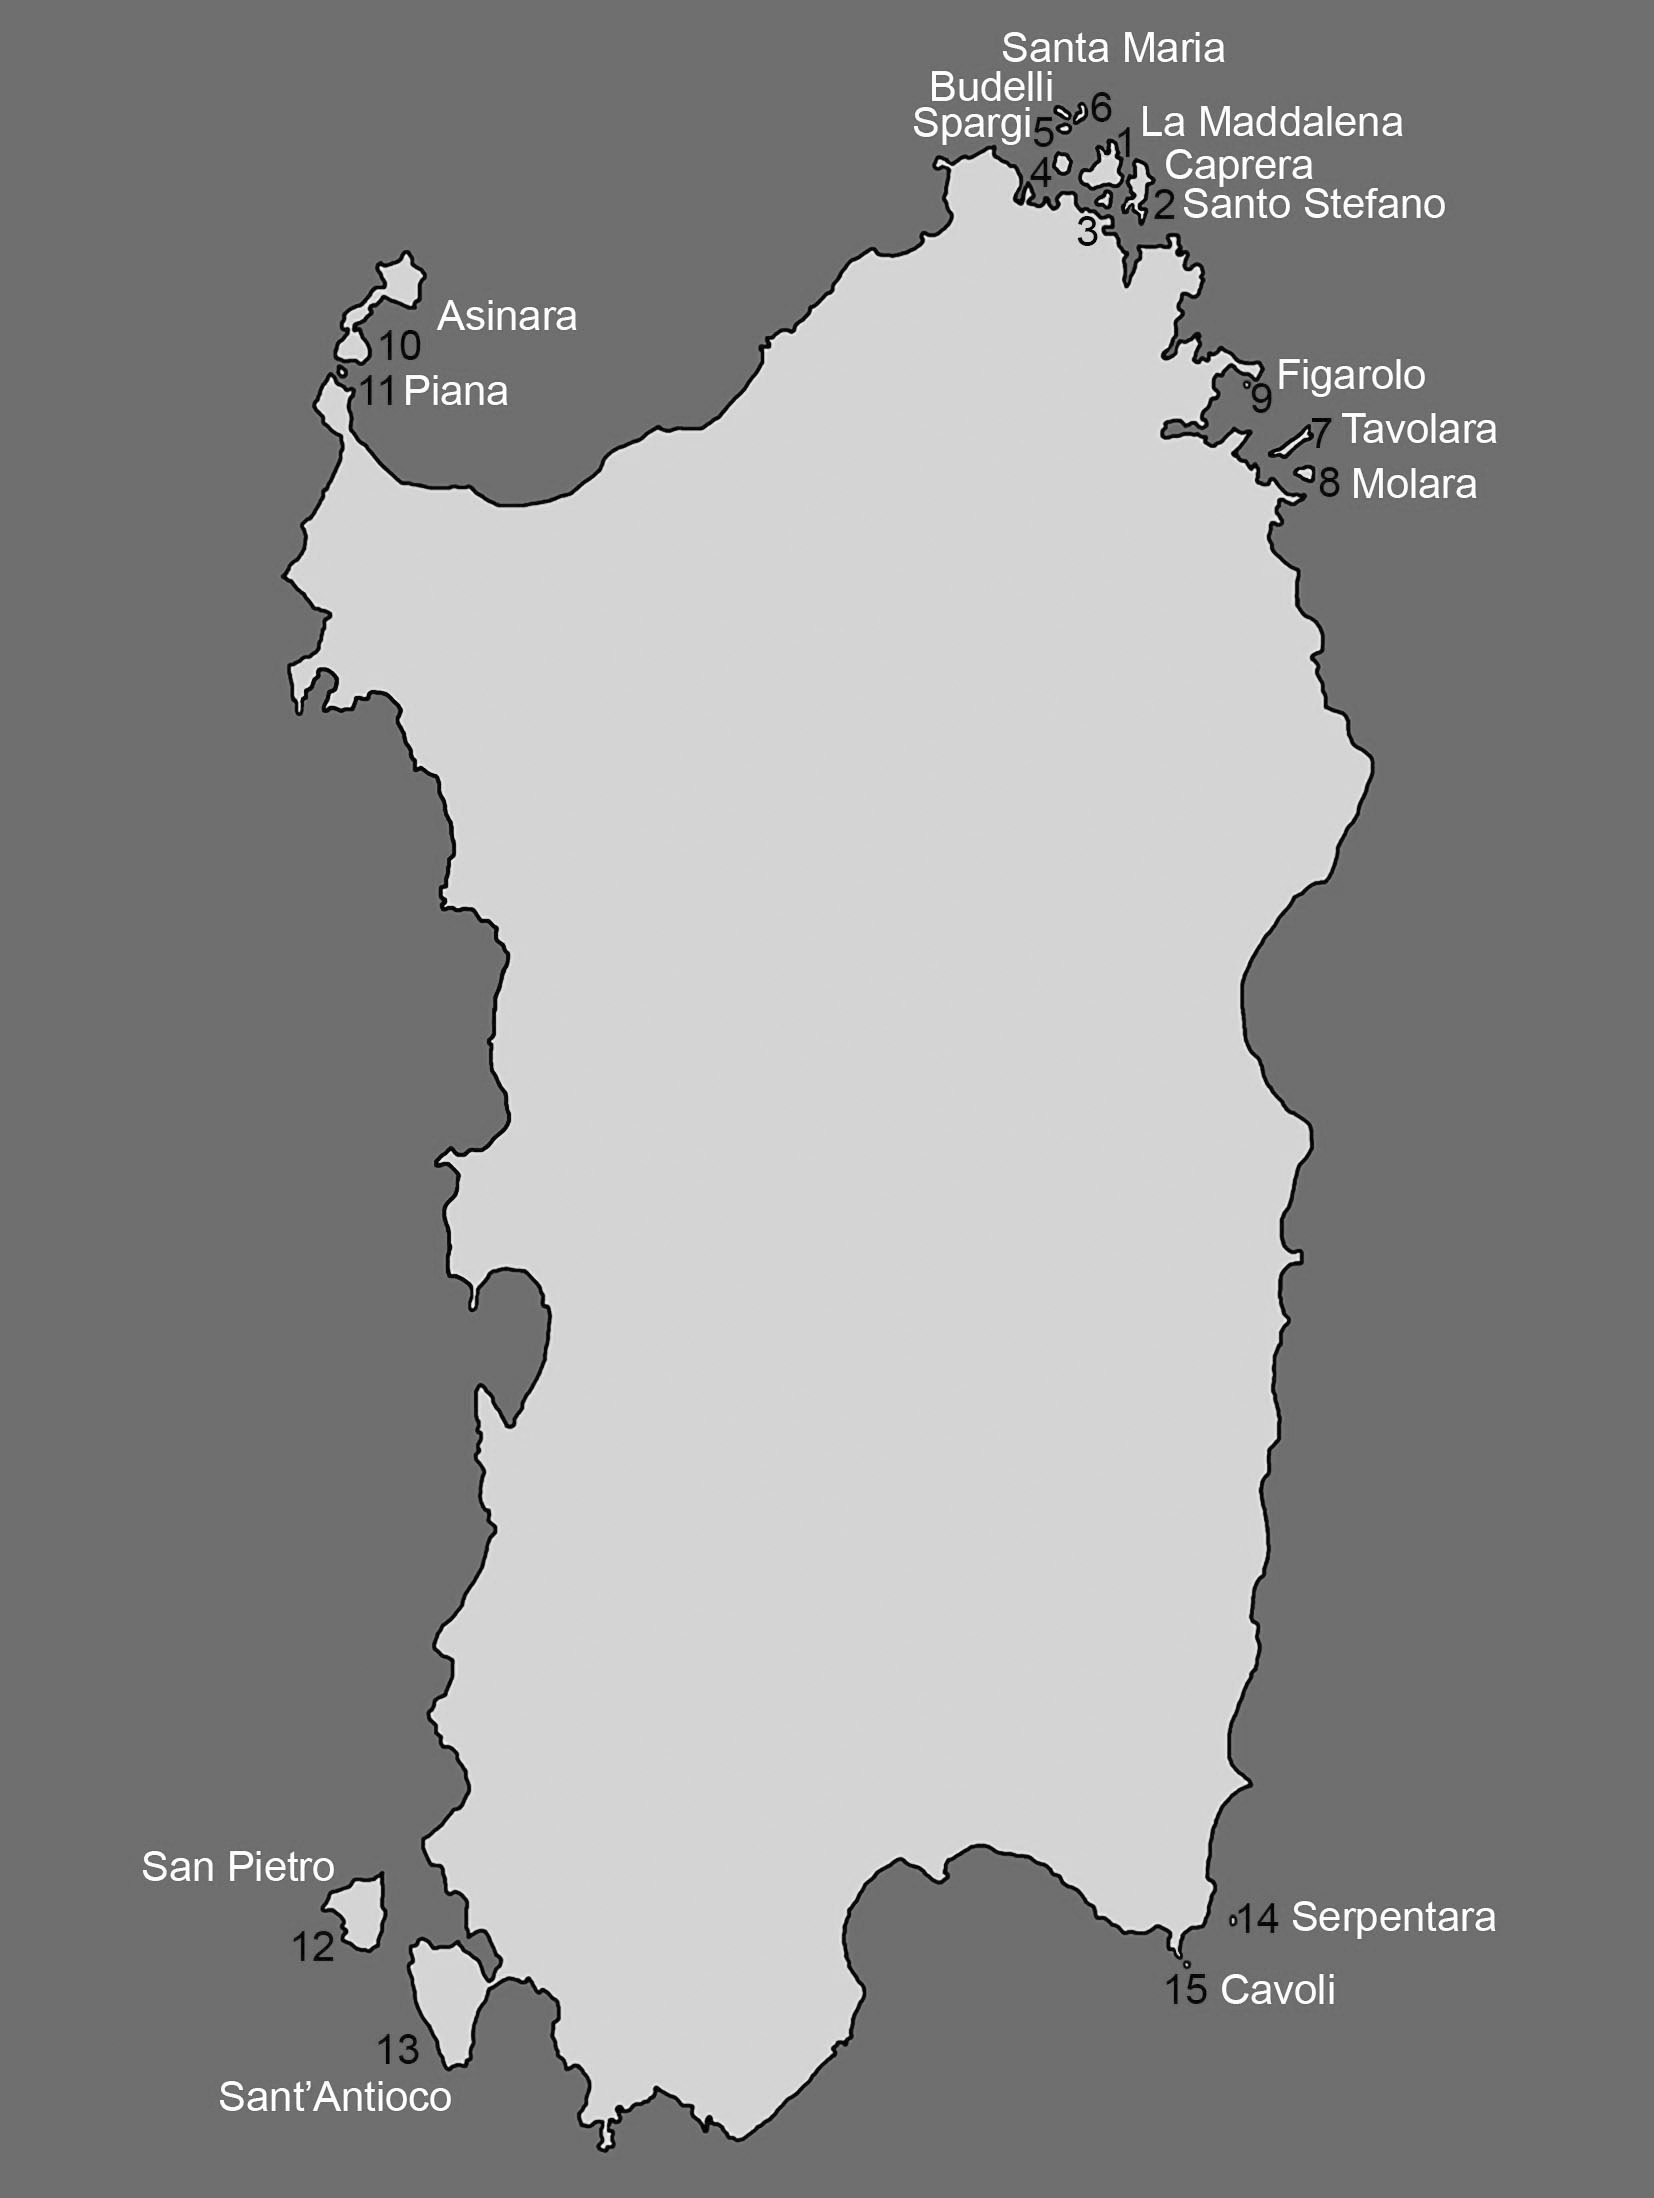
\includegraphics[width=\linewidth]{abstracts/extended_abstracts/C022_Figure1.png}
  \captionof*{}{Fig. 1 – Posizione geografica delle piccole isole della Sardegna.}
\end{Figure}

\section*{Risultati}
Riportiamo i risultati delle ricerche per ogni singola isola, a partire da nord verso sud.

\subsection*{Isola di La Maddalena (La Maddalena)}
È la principale isola dell’arcipelago, in cui ha sede la città di La Maddalena, con una popolazione di oltre 11000 abitanti. Ha una superficie di \SI{20.1}{\square\kilo\meter} e una quota massima di 212~m, ed è distante dalla costa sarda circa 2~km. Come tutte le isole dell’arcipelago è di natura granitica.

Le attività sono state effettuate in modo sporadico a partire dal 2005, e sono state completate con un monitoraggio della durata di un anno tra il 2010 e il 2011, finanziato dall’Ente Parco Nazionale dell’Arcipelago di La Maddalena. Le ricerche di rifugi di pipistrelli hanno interessato fortificazioni militari, edifici abbandonati, ruderi, civili abitazioni, gallerie, polveriere e riservette sotterranee, fessure nelle rocce.

Nell'Isola di La Maddalena sono stati localizzati 7 rifugi di pipistrelli, con la presenza di 4 specie.

Il monitoraggio col \textit{bat detector} è stato condotto in punti fissi di ascolto su un transetto in auto che si è svolto nelle strade sia lungo la cosa che nell’interno, compreso anche l'abitato.

In totale nell’isola, tra rifugi e monitoraggi notturni, è stata riscontrata la presenza di 7 specie di chirotteri:
\begin{compactdesc}
\item[\emph{Rhinolophus ferrumequinum}] osservato un solo esemplare in due diverse gallerie sotterranee, in letargo o riposo diurno.
\item[\emph{Myotis capaccinii}] pochi esemplari svernanti in una sola galleria sotterranea.
\item[\emph{Pipistrellus pipistrellus}] localizzato un rifugio con pochi esemplari in una galleria sotterranea e individuate quattro colonie in edifici, di cui solo due confermate come riproduttive; ampiamente contattato con il \textit{bat detector} ovunque nell’isola.
\item[\emph{Pipistrellus kuhlii}] ampiamente contattato con il \textit{bat detector} ovunque nell’isola.
\item[\emph{Hypsugo savii}], contattato con il \textit{bat detector} solo in poche località.
\item[\emph{Pipistrellus pygmaeus}/\emph{Miniopterus schreibersii}] pochi contatti registrati con il \textit{bat detector}, la cui analisi non ha consentito la discriminazione tra le due specie.
\item[\emph{Tadarida teniotis}] trovato un rifugio in una serie di fessure rocciose con almeno 35 individui osservati in uscita serale; contattato con il \textit{bat detector} nella parte occidentale dell’isola.
\end{compactdesc}

\subsection*{Isola di Caprera (La Maddalena - OL)}
È la seconda isola per importanza dell’arcipelago, con una superficie di \SI{15.7}{\square\kilo\meter} e una quota massima di 212~m. È collegata con un ponte a La Maddalena e ha una popolazione residente molto ridotta. 

Le attività sono state effettuate in modo sporadico a partire dal 2000, e sono state completate con un monitoraggio della durata di un anno tra il 2010 e il 2011, finanziato dall’Ente Parco Nazionale dell’Arcipelago di La Maddalena. Le ricerche di rifugi di pipistrelli hanno interessato fortificazioni militari, edifici abbandonati, ruderi, gallerie, polveriere e riservette sotterranee, fessure nelle rocce. 

Nell'Isola di Caprera sono stati individuati 14 rifugi di pipistrelli, con la presenza di 5 specie. Il monitoraggio col \textit{bat detector} è stato condotto in punti fissi di ascolto lungo tutte le strade dell’isola. 
In totale, tra rifugi e monitoraggi notturni, nell’Isola di Caprera è stata riscontrata la presenza di 8 specie.
\begin{compactdesc}
\item[\emph{Rhinolophus ferrumequinum}] osservato svernante o in riposo diurno, in numero di uno o due esemplari, in 7 gallerie sotterranee e 1 edificio.
\item[\emph{Rhinolophus hipposideros}] presente un solo esemplare in una struttura sotterranea militare.
\item[\emph{Myotis capaccinii}] osservato un solo esemplare in un vecchio edificio militare. 
\item[\emph{Pipistrellus pipistrellus}] osservato isolatamente in un rifugio sotterraneo e in tre edifici e catturato anche con le reti; è la specie più ampiamente contattata con il \textit{bat detector} ovunque nell’isola.
\item[\emph{Pipistrellus kuhlii}] contattato con il \textit{bat detector} in varie località.
\item[\emph{Hypsugo savii}] pochissimi contatti con il \textit{bat detector}.
\item[\emph{Pipistrellus pygmaeus}/\emph{Miniopterus schreibersii}] un solo contatto con il \textit{bat detector}.
\item[\emph{Tadarida teniotis}] presente una colonia di numero molto variabile in una fessura rocciosa, con max 38 esemplari conteggiati all’involo serale; contattato anche con il \textit{bat detector}.
\end{compactitem}

\subsection*{Isola di Santo Stefano (La Maddalena - OL)}
Ha una superficie di \SI{3}{\square\kilo\meter} e raggiunge la massima quota di 100~m. Distante 1~km dalla terraferma, l’isola non è disabitata, ma ha un insediamento turistico e una base militare.

Sono stati esplorati vari edifici abbandonati e una galleria sotterranea artificiale. Il monitoraggio col \textit{bat detector} è stato effettuato nell’agosto 2011 lungo un transetto a piedi sulle stradine dell’isola. 
In totale è stata riscontrata la presenza di 4 specie. 
\begin{compactdesc}
\item[\emph{Rhinolophus ferrumequinum}] osservato un solo esemplare in una galleria sotterranea.
\item[\emph{Pipistrellus pipistrellus}, \emph{Hypsugo savii} e \emph{Tadarida teniotis}] tutti con pochi contatti col \textit{bat detector} in diverse località.
\end{compactdesc}

\subsection*{Isola di Spargi (La Maddalena - OL)}
Con una superficie di \SI{4.2}{\square\kilo\meter} è la terza per estensione dell'Arcipelago, distante dalla costa 2.5~km. Raggiunge la quota massima di 153~m ed è normalmente disabitata, con qualche rara presenza umana limitata a soggiorno estivo.

Nell’Isola di Spargi le attività sono state svolte in maggio e in agosto 2011, con esplorazione di ruderi, vecchie strutture militari e una galleria sotterranea, in nessuna delle quali è stata riscontrata la presenza di pipistrelli.
Il monitoraggio col \textit{bat detector} è stato condotto con un transetto a piedi lungo i sentieri principali nella parte centrale e settentrionale dell’isola. Attività ridotta dei pipistrelli, con pochi contatti relativi a quattro specie registrate in diverse località: \emph{Pipistrellus pipistrellus}, \emph{Pipistrellus pygmaeus}/\emph{Miniopterus schreibersii}, \emph{Hypsugo savii} e \emph{Tadarida teniotis}.

\subsection*{Isola di Budelli (La Maddalena - OL)}
È distante circa 8~km dalla costa sarda, ha una superficie di \SI{1.6}{\square\kilo\meters} e si eleva sino alla quota di 88~m. Esiste una sola abitazione in cui vive il custode dell’isola.

Praticamente priva di potenziali rifugi, esplorate solamente due costruzioni e una fessura nella roccia.
Il monitoraggio col \textit{bat detector} è stato condotto nell’agosto 2011 lungo un transetto a piedi che ha interessato la parte orientale e centrale dell’isola. Pochi i contatti di pipistrelli, relativi a due sole specie in differenti località: \emph{Pipistrellus pipistrellus} più frequente e \emph{Tadarida teniotis}.

\subsection*{Isola di Santa Maria (La Maddalena - OL)}
È la più lontana dalla costa sarda, da cui dista 9~km, ha una superficie di \SI{2}{\square\kilo\meter} ed è la più bassa delle isole dell’arcipelago con una quota massima di soli 49 metri.

Sull’isola esistono una struttura alberghiera e poche abitazioni, utilizzate per lo più in periodo estivo.
Le ricerche di rifugi hanno interessato solamente 4 strutture edilizie, in nessuna delle quali è stata riscontrata la presenza di pipistrelli.

Il monitoraggio col \textit{bat detector} è stato realizzato nel luglio 2011 lungo un transetto a piedi nei sentieri che percorrono l’isola longitudinalmente. La registrazione dei suoni ha consentito di accertare la presenza di una sola specie di pipistrello: \emph{Pipistrellus pipistrellus}, contattata in diverse località.

\subsection*{Isola di Tavolara (Olbia - OL)}
Costituita da una basamento granitico, su cui si poggia un’imponente copertura calcarea mesozoica, che si eleva con carattere di montagna sino a 565~m di quota, la più alta di tutte le isole circumsarde. Situata a circa 2~km dalla costa, ha una superficie di \SI{5.9}{\square\kilo\meter}. Nella sua estremità di NE è sede di una base militare, mentre nella parte SO vi si trovano alcune case e alcune strutture di tipo turistico attive solo in periodo estivo.

Le prime ricerche sono state effettuate nel 1994 (Grafitti \& Mucedda, 1995) e sono riprese successivamente negli anni 2009-2013. Sono state esplorate alcune grotte ed edifici e sono stati effettuati tre monitoraggi notturni col \textit{bat detector} lungo transetti a piedi nell’unica stradina e sui sentieri nella sola parte SO non militarizzata dell’isola.
È stata riscontrata la presenza di 8 specie di pipistrelli. 
\begin{compactdesc}
\item[\emph{Rhinolophus ferrumequinum}] presente con un solo esemplare nella grotta Inghiottitoio della Mandria e nella vicina Grotta Findema.
\item[\emph{Miniopterus schreibersii}] osservati una decina di esemplari nella Grotta dei Fiori d’Arancio.
\item[\emph{Pipistrellus pipistrellus} e \emph{Pipistrellus kuhlii}] sono le specie più frequentemente contattate con il \textit{bat detector} in varie località, anche sulla spiaggia.
\item[\emph{Hypsugo savii} e \emph{Tadarida teniotis}] contattate con il \textit{bat detector}, meno frequenti delle due specie precedenti. 
\item[\emph{Myotis} indet.] un solo contatto che non ha consentito di identificare la specie.
\item[\emph{Eptesicus serotinus}] contattato ripetutamente in caccia su un’area pinetata. Si ritiene valida l’identificazione grazie a numerose registrazioni in successione, in cui non si evidenzia mai alternanza delle due tipologie di segnali, escludendo così che si possa trattare di \emph{Nyctalus leisleri} con cui può essere facilmente confuso.
\end{compactdesc}

\subsection*{Isola di Molara (Olbia - OL)}
Di natura granitica, ha una superficie di \SI{3.4}{\square\kilo\meter} e raggiunge la massima quota di 155~m. È distante dalla costa circa 2~km ed è disabitata.

Le ricerche si sono svolte con il controllo di alcuni edifici, che non hanno rivelato tracce di pipistrelli, e con una sola notte di registrazioni col \textit{bat detector}, lungo un transetto a piedi sui sentieri, nell’agosto 2012. È stata riscontrata la presenza di 3 specie: 
\begin{compactdesc}
\item[\emph{Pipistrellus pipistrellus}] ampiamente presente in tutta l’isola. 
\item[\emph{Hypsugo savii}] un solo contatto nella parte sommitale dell’isola.
\item[\emph{Tadarida teniotis}] registrato in diverse località.
\end{compactdesc}

\subsection*{Isola di Figarolo (Golfo Aranci - OL)}
Minuscola isoletta disabitata, con una superficie di \SI{0.2}{\square\kilo\meter}, la più piccola tra quelle visitate, situata a soli 350~m dalla costa. Geologicamente ha un basamento granitico sul quale poggiano delle bancate calcaree dell’era Mesozoica, con vegetazione a macchia mediterranea e fitte aree boscate, che raggiunge la massima quota di 139~m.
  
Le ricerche hanno interessato una sola notte di registrazioni col \textit{bat detector}, lungo un transetto a piedi, nell’agosto 2014.
Nonostante le sue ridotte dimensioni vi è stata riscontrata la presenza di 4 specie: \emph{Pipistrellus pipistrellus}, \emph{Pipistrellus kuhlii}, \emph{Hypsugo savii} e \emph{Tadarida teniotis}, tutte con contatti poco numerosi.

\subsection*{Isola dell'Asinara (Porto Torres - SS)}
Costituisce un Parco Nazionale, con una superficie di \SI{51}{\square\kilo\meter} e non ha una popolazione residente, ma solo attività legate alla valorizzazione turistica e alla tutela ambientale. Di natura granitica e scistosa, raggiunge la massima altitudine di 408~m.

Nell’Isola dell’Asinara sono state effettuate ricerche saltuarie a partire dal 1995, proseguite poi in modo più approfondito dal 2008 al 2015.
Le ricerche si sono basate sulla individuazione dei rifugi di pipistrelli, catture con le reti e registrazioni notturne col \textit{bat detector}. Negli ultimi anni le attività sono state condotte in collaborazione con Rebecca Winter, che ha svolto sull’isola intense indagini triennali per il suo Dottorato presso l’Università di Hildesheim in Germania. 

Sono stati localizzati 30 rifugi in edifici e altre strutture e 2 in piccole cavità sotterranee artificiali. 
In totale sono state individuate 10 specie di pipistrelli: 
\begin{compactdesc}
\item[\emph{Rhinolophus ferrumequinum}] osservato in numero molto ridotto di esemplari in edifici e in cavità sotterranee artificiali, per un totale di 10 rifugi.
\item[\emph{Rhinolophus hipposideros}] è la specie più numerosa negli edifici abbandonati, osservata anche in cisterne. Individuati 11 rifugi e 2 colonie di riproduzione, con un massimo di circa 40 esemplari presenti. Contattato anche con il \textit{bat detector}.
\item[\emph{Myotis daubentonii}] osservato in tutti i laghetti presenti sull’isola e catturato con le reti in pochi esemplari. 
\item[\emph{Miniopterus schreibersii}] catturato un solo esemplare con le reti. 
\item[\emph{Pipistrellus pipistrellus}] è la specie più ampiamente contattata con il \textit{bat detector} ovunque nell’isola. Utilizza anche edifici, con piccole colonie che si annidano generalmente dietro le grondaie. Catturato anche con le reti.
\item[\emph{Pipistrellus kuhlii}] è la seconda specie più ampiamente contattata con il \textit{bat detector}, catturato anche con le reti. 
\item[\emph{Pipistrellus pygmaeus}] pochi contatti con il \textit{bat detector}, identificato dall’analisi dei \textit{social calls}. 
\item[\emph{Hypsugo savii}] pochissimi contatti con il \textit{bat detector}. 
\item[\emph{Eptesicus serotinus} o \emph{Nyctalus leisleri}] pochissimi contatti con il \textit{bat detector}. Dai soli suoni registrati non è stato possibile discriminare tra le due specie.
\item[\emph{Tadarida teniotis}] contattato con il \textit{bat detector} in varie parti dell’isola. 
\end{compactdesc}

\subsection*{Isola Piana (Porto Torres - SS)}
Piccola isoletta che ha una superficie di \SI{1.4}{\square\kilo\meter}, è situata a 600~m dalla costa ed è disabitata. È di natura scistosa, con bassa e rada vegetazione a macchia mediterranea, che si eleva solo sino a 24 di quota. 

Le ricerche sono state effettuate per una sola notte nell’agosto 2015. Controllata la Torre spagnola, l’unica struttura edilizia presente che è risultata priva di pipistrelli.
L’attività notturna dei pipistrelli si è rivelata inizialmente abbondante su una piccola polla d’acqua nella parte nord dell’isola, poi scarsa con pochi contatti al \textit{bat detector}.
Lungo un transetto a piedi che ha interessato quasi tutta l’isola è stata rilevata la presenza di due sole specie: \emph{Pipistrellus pipistrellus} più frequente e \emph{Pipistrellus kuhlii} meno frequente. 

\subsection*{Isola di San Pietro (Carloforte - CI)}
È un’isola di natura vulcanica di \SI{51}{\square\kilo\meter} di superficie ed è abitata, con la cittadina di Carloforte che ha circa 6500 abitanti. È distante circa 7~km dalla costa sarda e ha la massima altitudine di 211~m.

Nell’Isola di San Pietro le nostre attività hanno avuto inizio nel 1995 e si sono protratte in modo saltuario sino al 2013. Le ricerche si sono articolate con l’individuazione di rifugi di pipistrelli e registrazioni notturne col \textit{bat detector}, lungo transetti in auto che hanno interessato tutta l’isola.
È stata accertata la presenza di 5 specie di pipistrelli: 
\begin{compactdesc}
\item[\emph{Rhinolophus hipposideros}] è stato osservato in due gallerie minerarie e registrato in attività notturna col \textit{bat detector}. 
\item[\emph{Myotis capaccinii}] presenti piccoli gruppi di qualche decina di esemplari in una galleria mineraria. 
\item[\emph{Pipistrellus pipistrellus}] è la specie più ampiamente contattata con il \textit{bat detector} in tutta nell’isola. 
\item[\emph{Pipistrellus kuhlii}] pochi contatti con il \textit{bat detector}. 
\item[\emph{Tadarida teniotis}] contattata con il \textit{bat detector} in varie parti dell’isola. 
\end{compactdesc}

\subsection*{Isola di Sant'Antioco (Sant'Antioco e Calasetta – CI)}
Sant'Antioco con una superficie di \SI{108.9}{\square\kilo\meter} è una delle maggiori isole italiane, con due centri abitati, Sant’Antioco e Calasetta, e una popolazione totale di oltre 14000 abitanti. È collegata alla terraferma con un istmo e un ponte, è di natura prevalentemente vulcanica con ridotti lembi calcarei e raggiunge la massima quota di 273~m.

Le attività sono state effettuate negli anni 2002, 2006, 2010 e 2014. Le ricerche di rifugi di pipistrelli hanno interessato alcune grotte, edifici abbandonati, la necropoli punica. Le catture con le reti sono state effettuate in una sola occasione in un laghetto. Le registrazioni notturne con \textit{bat detector} sono state realizzate lungo transetti in auto in tre diverse occasioni e hanno interessato quasi tutta l’isola.
In totale è stata accertata la presenza a Sant’Antioco di 6 specie di chirotteri: 
\begin{compactdesc}
\item[\emph{Rhinolophus hipposideros}] è stato osservato isolatamente in due sole cavità sotterranee, una tomba della Necropli Punica e la Grotta di Sargaltas. 
\item[\emph{Miniopterus schreibersii}] un solo esemplare rinvenuto all’esterno di un edificio nel centro abitato di Sant’Antioco.
\item[\emph{Pipistrellus pipistrellus}] contattato con \textit{bat detector} ovunque nell’isola, catturato anche con le reti. 
\item[\emph{Pipistrellus kuhlii}] contattato con il \textit{bat detector} meno frequentemente della specie precedente. 
\item[\emph{Hypsugo savii}] contattato con il \textit{bat detector} in poche località. 
\item[\emph{Tadarida teniotis}] contattato con il \textit{bat detector} solo in poche occasioni. 
\end{compactdesc}
A questo elenco si deve aggiungere il \emph{Myotis punicus}, già citato da Zava et Al. (1996) e segnalato anche da Skiba (2009), di cui noi non abbiamo accertato la presenza attuale sull’isola.

\subsection*{Isola di Serpentara (Villasimius – CA)}
È un’isola molto piccola, con una superficie di solo \SI{1.34}{\square\kilo\meter}, che raggiunge la massima quota di 54~m e dista poco più di 3~km dalla costa sarda. È di natura granitica, con vegetazione a macchia mediterranea ed è disabitata. 

Le ricerche sono state effettuate per una sola giornata e una notte nell’agosto 2013. Controllate la torre spagnola, unico edificio presente, e piccole cavità e tafoni; non è stato individuato alcun rifugio di pipistrelli né tracce della loro presenza.
Lungo un transetto a piedi che ha interessato quasi tutta l’isola è stata rilevata la presenza di due sole specie: \emph{Pipistrellus pipistrellus} e \emph{Tadarida teniotis}.

\begin{table*}[t]
\caption*{Tab. 1 - Elenco delle specie rilevate per ciascuna delle isole monitorate. N\degree{}: numero di specie rilevate. L'ultima riga indica il numero di isole su cui è stata rilevataciascuna specie. Rfe=\emph{Rhinolophus ferrumequinum}; Rhi=\emph{Rhinolophus hipposideros}; Mca=\emph{Myotis capaccinii}; Mda=\emph{Myotis daubentonii}; Myo=\emph{Myotis} sp.; Msc=\emph{Miniopterus schreibersii}; Ppi=\emph{Pipistrellus pipistrellus}; Pku=\emph{Pipistrellus kuhlii}; Hsa=\emph{Hypsugo savii}; Ppyg=\emph{Pipistrellus pygmaeus}; Ese=\emph{Eptesicus serotinus}; Tte=\emph{Tadarida teniotis}.}
%\label{tab:table1}
\centering\small
\begin{tabular}{lccccccccccccc}
\quad & \textbf{N\degree{}} & \textbf{Rfe} & \textbf{Rhi} & \textbf{Mca} & \textbf{Mda} & \textbf{Myo} & \textbf{Msc} & \textbf{Ppi} & \textbf{Pku} & \textbf{Ppyg} & \textbf{Hsa} & \textbf{Ese} & \textbf{Tte} \\
\hline
La Maddalena  &  7 & $\times$ &          & $\times$ &          &          &          & $\times$ & $\times$ & $\times$? & $\times$ &           & $\times$ \\
Caprera       &  8 & $\times$ & $\times$ & $\times$ &          &          &          & $\times$ & $\times$ & $\times$? & $\times$ &           & $\times$ \\
Santo Stefano &  4 & $\times$ &          &          &          &          &          & $\times$ &          &           & $\times$ &           & $\times$ \\
Spargi        &  2 &          &          &          &          &          &          & $\times$ &          & $\times$? & $\times$ &           & $\times$ \\
Budelli       &  2 &          &          &          &          &          &          & $\times$ &          &           &          &           & $\times$ \\
Santa Maria   &  1 &          &          &          &          &          &          & $\times$ &          &           &          &           &          \\
Tavolara      &  8 & $\times$ &          &          &          & $\times$ & $\times$ & $\times$ & $\times$ &           & $\times$ & $\times$  & $\times$ \\
Molara        &  3 &          &          &          &          &          &          & $\times$ &          &           & $\times$ &           & $\times$ \\
Figarolo      &  4 &          &          &          &          &          &          & $\times$ & $\times$ &           & $\times$ &           & $\times$ \\
Asinara       & 10 & $\times$ & $\times$ &          & $\times$ &          & $\times$ & $\times$ & $\times$ & $\times$  & $\times$ & $\times$? & $\times$ \\
Piana         &  2 &          &          &          &          &          &          & $\times$ & $\times$ &           &          &           &          \\
San Pietro    &  5 &          & $\times$ & $\times$ &          &          &          & $\times$ & $\times$ &           &          &           & $\times$ \\
Sant’Antioco  &  6 &          & $\times$ &          &          &          & $\times$ & $\times$ & $\times$ &           & $\times$ &           & $\times$ \\
Serpentara    &  2 &          &          &          &          &          &          & $\times$ &          &           &          &           & $\times$ \\
Cavoli        &  2 &          &          &          &          &          &          & $\times$ & $\times$ &           &          &           &          \\
N\degree{} isole &    &        5 &        4 &        3 &        1 &        1 &        3 &       15 &        9 &         4 &        9 &         2 &       12 \\
\end{tabular}
\end{table*}

\subsection*{Isola dei Cavoli (Villasimius – CA)}
Minuscola isola con una superficie di \SI{0.43}{\square\kilo\meter}, è distante solo 700~m dalla estrema punta sud orientale della Sardegna ed è disabitata. È di natura granitica, con bassa vegetazione a macchia mediterranea, e raggiunge solo la quota di 40~m.
 
Le ricerche sono state effettuate per una sola giornata e una notte nel luglio 2012. Nelle due uniche strutture edilizie presenti non è stato individuato alcun rifugio di pipistrelli.
Lungo un transetto a piedi che ha interessato tutta l’isola sono stati registrati pochissimi contatti che hanno rivelato la presenza di due sole specie: \emph{Pipistrellus pipistrellus} e \emph{Pipistrellus kuhlii}.

A queste 15 si devono aggiungere l’Isola di Razzoli e l’isolotto del Porco nell’Arcipelago di La Maddalena e l’isolotto della Foradada nel comune di Alghero, in cui sono state fatte solo prospezioni diurne che non hanno rivelato la presenza di pipistrelli.

\section*{Discussione}
Su 21 specie di chirotteri presenti nella Sardegna, almeno 11 sono state riscontrate nel totale delle isole minori.
\begin{compactitem}
\item Rinolofo maggiore (\emph{Rhinolophus ferrumequinum} Schreber, 1774)
\item Rinolofo minore (\emph{Rhinolophus hipposideros} Bechstein, 1800)
\item Vespertilio di Capaccini (\emph{Myotis capaccinii} Bonaparte, 1837)
\item Vespertilio di Daubenton (\emph{Myotis daubentonii} Kuhl, 1819)
\item Pipistrello nano (\emph{Pipistrellus pipistrellus} Schreber, 1774)
\item Pipistrello albolimbato (\emph{Pipistrellus kuhlii} Kuhl, 1817)
\item Pipistrello pigmeo (\emph{Pipistrellus pygmaeus} Leach, 1825)
\item Pipistrello di Savi (\emph{Hypsugo savii} Bonaparte, 1837)
\item Serotino comune (\emph{Eptesicus serotinus} Schreber, 1774) o Nottola di Leisler (\emph{Nyctalus leisleri} Kuhl, 1818)
\item Miniottero (\emph{Miniopterus schreibersii} Kuhl, 1817)
\item Molosso di Cestoni (\emph{Tadarida teniotis} Rafinesque, 1814)
\end{compactitem}

Tra le specie contattate solamente col \textit{bat detector}, alcune non è stato possibile identificarle con certezza. È il caso della coppia \emph{Pipistrellus pygmaeus}---\emph{Miniopterus schreibersii} per l’Arcipelago di La Maddalena e \emph{Eptesicus serotinus}---\emph{Nyctalus leisleri} per l’Asinara, considerate come un’unica entità in quanto non è stato possibile distinguerle sulla base delle loro emissioni ultrasonore, per cui nel conteggio delle specie si intende presente l’una o l’altra delle due. Il \emph{Pipistrellus pygmaeus} all’Asinara è stato invece identificato con certezza sulla base dei \textit{social calls}. 

Come già detto in precedenza, si ritiene valida anche l’identificazione di \emph{Eptesicus serotinus} a Tavolara, le cui registrazioni non evidenziano mai alternanza delle due tipologie di segnali.

Nella Tab. 1 si riportano per ognuna delle 15 isole monitorate, da nord a sud, le specie di pipistrelli da noi riscontrate come presenti. 

La seconda colonna della Tab. 1 (N\degree{}) mostra il numero di specie presenti in ogni singola isola; l’ultima riga indica il numero di isole in cui è presente ogni singola specie.

Il più alto numero di specie si riscontra all’Asinara con 10 entità, seguita da Caprera e Tavolara con 8, quindi La Maddalena con 7. Nelle altre isole il numero va a diminuire, riducendosi notevolmente nelle isolette più piccole sino al minimo di una sola specie.

In un’ampia visione che riguarda tutta l’Italia, sulla base di quanto pubblicato da Angelici et al. (2009), l’Asinara (10 specie) detiene il più elevato numero di entità alla pari con l’Isola d’Elba, Caprera e Tavolara (8 specie) superano l’Isola del Giglio (7 specie) che è alla pari con La Maddalena. Come particolarità, nelle isole sarde compaiono \emph{Myotis capaccinii}, \emph{Myotis daubentonii} e \emph{Pipistrellus pygmaeus} che non risultano sinora presenti in altre piccole isole italiane.

Le specie più ampiamente diffuse sono \emph{Pipistrellus pipistrellus}, presente in tutte le isole, seguita da \emph{Tadarida teniotis} in 12 isole, \emph{Hypsugo savii} e \emph{Pipistrellus kuhlii} in 9 isole. La più rara è risultata invece \emph{Myotis daubentonii} presente solo all’Asinara.

La specie troglofila più diffusa è \emph{Rhinolophus ferrumequinum}, presente in 5 isole.

Facendo un ulteriore confronto con le altre 26 isole italiane citate in Angelici et al. (2009), a differenza di quelle sarde in ambito italiano il più diffuso è \emph{Pipistrellus kuhlii} presente in 20 isole, mentre \emph{Pipistrellus pipistrellus} è presente in sole 11 isole, seguito da \emph{Tadarida teniotis} in 10 isole. 

Dal nostro studio emerge che la maggior parte dei contatti con i chirotteri nelle isole circumsarde avviene mediante l’uso del \textit{bat detector}. Se andiamo a valutare la somma delle specie contattate nella totalità delle isole, emerge infatti che su un valore cumulato di 68 identificazioni di specie, quelle contattate solo con \textit{bat detector} ammontano a 43, mentre quelle identificate mediante osservazione diretta nei rifugi o cattura sono 19 e quelle identificate con entrambi i metodi sono 6. Si sottolinea pertanto l’importanza crescente del metodo di identificazione bioacustica nei monitoraggi della chirotterofauna, anche se non sempre si può giungere ad una identificazione certa delle specie contattate.

Le isole oggetto dello studio ricadono tutte all’interno di aree protette. Più esattamente La Maddalena, Caprera, Santo Stefano, Spargi, Budelli e Santa Maria sono all’interno del Parco Nazionale dell’Arcipelago di La Maddalena; Tavolara e Molara ricadono nell’Area Marina Protetta Tavolara-Capo Coda Cavallo; Figarolo appartiene al Sito di Interesse Comunitario di Capo Figari; Asinara è Parco Nazionale, area SIC e ZPS; Piana è compresa nell’area SIC dell’Asinara; San Pietro è interamente Sito di Interesse Comunitario; Sant’Antioco presenta varie aree SIC che interessano parzialmente il suo territorio; Serpentara e Cavoli ricadono entrambe nell’Area Marina Protetta di Capo Carbonara.

\vskip3mm

\begin{small}
\noindent\textbf{Ringraziamenti}\\
Le ricerche sulle isole si sono avvalse della collaborazione preziosa di un gran numero di persone ed Enti che qui ringraziamo riportandoli in ordine sparso. Parco Nazionale dell’Arcipelago di La Maddalena, Antonella Gaio, Luca Bittau, Valentina Gilioli, Gaetano Pedroni, Alessandro Ragni, Mauro Morandi, Tommaso Gamboni, Irene Galante, Francesco Muzzu, Laura Aversano, Paolo Agnelli, Giuseppe Are, Parco Nazionale dell’Asinara, Pierpaolo Congiatu, Giovanni Careddu, Giuseppe Grieco, Danilo Pisu, Cristina Fiesoli, Angelo Pittalis, Veronica Pisu, Antonio Guiso, Stefania Piras, Simone Rosa, Giuliana Atzori, Anna Laura Tanca, Rebecca Winter, Julia Treitler, Tim Drissen, Robin Stadtmann, Area Marina Protetta di Tavolara e Capo Coda Cavallo, Giovanna Spano, Massimo Putzu, Diego Gaia, Area Marina Protetta di Capo Carbonara, Bruno Paliaga, Fabrizio Atzori, Soprintendenza Archeologica di Cagliari, Luciano Durante, Sandro Mezzolani, Francesco Livretti, Marco Siddi, Giorgio Bardelli, Gaetano Fichera, Luca Montanaro, Enrico Melis, Alessio Sale. 

\vskip3mm

\noindent\textbf{Bibliografia}\\

Angelici F.M., Laurenti A., Nappi A., 2009. A checklist of the mammals of small italian islands. Hystrix 20(1): 3--27.

Barataud M., 2012. Ecologie acoustique des chiropteres d’Europe. Biotope editions: 343 pp.

Grafitti G., Mucedda M., 1995. Le grotte dell'Isola di Tavolara e la loro fauna. Biogeographia XVIII: 51--62.

Mocci Demartis A., Secci A., 1997. Dati sulla distribuzione dei Chirotteri nella Sardegna meridionale. Rend. Sem. Fac. Scienze Univ. Di Cagliari, 67: 61--74.

Russo D, Jones G., 2002. Identification of twenty-two bat species (Mammalia: Chiroptera) from Italy by analysis of time-expanded recordings of echolocation calls. J. Zool., London, 258: 91--103.

Skiba R., 2009. Europäische Fledermäuse. Westarp Wissenschaften: 128.

Zava B., Fiore M., Fornasari L., Violani C., 1996. Note sui Chirotteri dell'Isola di San Pietro con cenni storici sulle ricerche chirotterologiche in Sardegna. Biogeographia, XVIII: 641--651.

Zava B., Violani C., 1992. Nuovi dati sulla chirotterofauna italiana. Boll. Mus. Reg. Sci. Nat. Torino, 10 (2): 261-264.

\end{small}

\end{multicols}
% % EOF % %


\conferenceday{Venerdì 9 ottobre 2015}

%%%%%%%%%%%%%%%%%%%%%%%%%%%%%%%%%%%%%%%%%%%%%%%%%%%%%%%%%%%%%%%%%%%%%%%%%%%%%%%
\sessionname[Parassitologia ed Epidemiologia]{Parassitologia ed Epidemiologia}
\noindent\textbf{Coordinatori}\\
Marco \textsc{Riccucci}, Dino \textsc{Scaravelli}
\medskip

%% abstracts here
%% load an abstract [text on abstract margin]{TOC entry}{include file}
%\loadabstr[TEST]{Authors --- Title}{abstracts/gestione/G_119.tex}

%\loadabstr[Opening lecture]{Opening Lecture: Eric \textsc{Baubet} - \textit{Title to be confirmed}}{abstracts/gestione/G_000_Baubet.tex}
%% File created by make_summary.R script
%% Include in the main.tex file
\loadabstr[C020]{LEOPARDI S., BLAKE D., PUECHMAILLE S. -- The relevance of White Nose Syndrome in Europe}{abstracts/comunicazioni_parassitologia/C020_leopardi.ea.tex}
\loadabstr[C021]{LEOPARDI S., PRIORI P., SCARAVELLI D., ZECCHIN B., CATTOLI G., DE BENEDICTIS P. -- Bat lyssaviruses circulation in European bats: is there an actual conflict between species conservation and public health?}{abstracts/comunicazioni_parassitologia/C021_leopardi.ea.tex}
\loadabstr[E026]{RIZZO F., ROBETTO S., GUIDETTI C., LO VECCHIO C., ZOPPI S., DONDO A., BALLARDINI M., MIGNONE W., BERTOLOTTI L., ROSATI S., CALVINI M., TOFFOLI R., ORUSA R., MANDOLA M.L. -- Individuazione di Alphacornavirus nella chirotterofauna nord-occidentale: risultati preliminari}{abstracts/comunicazioni_parassitologia/E026_rizzo.ea.tex}
\loadabstr[C043]{PRIORI P., GUIDI L., SCARAVELLI D. -- Parametri ecologici condizionanti la comunit� ectoparassitaria in colonie italiane di chirotteri}{abstracts/comunicazioni_parassitologia/C043_priori.ea.tex}
\loadabstr[C048]{DE MARCO M.A., CASTRUCCI M.R. -- Il ruolo dei chirotteri nell'ecologia dei coronavirus emergenti}{abstracts/comunicazioni_parassitologia/C048_demarco.tex}


\cleardoublepage


\conferenceday{Sabato 10 ottobre 2015}

%%%%%%%%%%%%%%%%%%%%%%%%%%%%%%%%%%%%%%%%%%%%%%%%%%%%%%%%%%%%%%%%%%%%%%%%%%%%%%%
\sessionname[Modellistica]{Modellistica}
\noindent\textbf{Coordinatori}\\
Damiano \textsc{Preatoni}, Federica \textsc{Roscioni}
\medskip

%% abstracts here
%% load an abstract [text on abstract margin]{TOC entry}{include file}
%\loadabstr[TEST]{Authors --- Title}{abstracts/gestione/G_119.tex}

%\loadabstr[Opening lecture]{Opening Lecture: Eric \textsc{Baubet} - \textit{Title to be confirmed}}{abstracts/gestione/G_000_Baubet.tex}
%% File created by make_summary.R script
%% Include in the main.tex file
\loadabstr[C011]{ANCILLOTTO L., SANTINI L., RANC N., MAIORANO L., TOMASSINI A., RUSSO D. -- A winner bat in a changing environment: local and global responses of \emph{Pipistrellus kuhlii} to urbanization and climate change}{abstracts/comunicazioni_modellistica/C011_ancillotto.ea.tex}
\loadabstr[C029]{DUCCI L., AGNELLI P., DI FEBBRARO M., FRATE L., RUSSO D., CARRANZA M.L., LOY A., SANTINI G., ROSCIONI F. -- Testing the effectiveness of protected areas to preserve bat habitat and commuting routes: a region-scale model for the aerial-hawke \emph{Nyctalus noctula}}{abstracts/comunicazioni_modellistica/C029_ducci.ea.tex}
\loadabstr[C027]{PICCIOLI CAPPELLI M., MARTINOLI A., RUSSO D., REBELO H. -- Evaluating the impact of climate change on species distribution. A study on the Mediterranean bat community of Western Palaearctic}{abstracts/comunicazioni_modellistica/C027_piccioli.ea.tex}
\loadabstr[C003]{RUSSO D., DI FEBBRARO M., CISTRONE L., JONES G., SMERALDO S., GARONNA A.P., BOSSO L. -- Protecting one, protecting both? Scale-dependent ecological differences in two species using dead trees, the \emph{Rosalia} longicorn beetle and the Barbastelle bat}{abstracts/comunicazioni_modellistica/C003_russo.tex}


\cleardoublepage

\sessionname[Ecologia e Comportamento]{Ecologia e Comportamento}
\noindent\textbf{Coordinatori}\\
Leonardo \textsc{Ancillotto}, Mauro \textsc{Mucedda}, Danilo \textsc{Russo}
\medskip

%% abstracts here
%% load an abstract [text on abstract margin]{TOC entry}{include file}
%\loadabstr[TEST]{Authors --- Title}{abstracts/gestione/G_119.tex}

%\loadabstr[Opening lecture]{Opening Lecture: Eric \textsc{Baubet} - \textit{Title to be confirmed}}{abstracts/gestione/G_000_Baubet.tex}
%% File created by make_summary.R script
%% Include in the main.tex file
\loadabstr[C004]{RUSSO D., ANCILLOTTO L., CISTRONE L., KORINE C. -- The buzz of drinking on the wing in echolocating bats}{abstracts/comunicazioni_ecologia/C004_russo.tex}
\loadabstr[C002]{RICCUCCI M. -- Play in Bats: general overview, current knowledge and future challenges}{abstracts/comunicazioni_ecologia/C002_riccucci.tex}
\loadabstr[C012]{STUDER V., MANZIA F., RENZOPAOLI F., TOMASSINI A., ANCILLOTTO L. -- Bat rescue and research: weaknesses and opportunities}{abstracts/comunicazioni_ecologia/C012_studer.ea.tex}
\loadabstr[C031]{GIACOMINI G., PRIORI P., SCARAVELLI D. -- Bat bioacoustic studies in Buenos Aires province, Argentina}{abstracts/comunicazioni_ecologia/C031_giacomini.ea.tex}
\loadabstr[C024]{CAMPEDELLI T., GUGLIELMO L. , CUTINI S., SCARAVELLI D., PRIORI P., TELLINI FLORENZANO G. -- Composizione forestale e comunit� dei chirotteri nel Parco Nazionale delle Foreste Casentinesi, Monte Falterona e Campigna: il ruolo dei boschi di conifere}{abstracts/comunicazioni_ecologia/C024_campedelli.ea.tex}
\loadabstr[C034]{WINTER R., TREITLER J., KIERDORF U., SCHMIDT S., MANTILLA-CONTRERAS J. -- Occurrence and activity patterns of bats in different habitat types in the northern part of the island of Asinara (Sardinia, Italy)}{abstracts/comunicazioni_ecologia/C034_winter.ea.tex}
\loadabstr[C010]{FERRI V. -- Bats of Reatini Mountains: diversity and abundance by elevation (Central Italy, NE Latium)}{abstracts/comunicazioni_ecologia/C010_ferri.tex}
\loadabstr[C013]{NARDONE V., RUSSO D., IBA\~NEZ C., JUSTE J. -- A first approach to the phylogeography of Daubenton's bat \emph{Myotis daubentonii}}{abstracts/comunicazioni_ecologia/C013_nardone.ea.tex}


\cleardoublepage

\sessionname[Distribuzione e Conservazione]{Distribuzione e Conservazione}
\noindent\textbf{Coordinatori}\\
Paolo \textsc{Agnelli}, Martina \textsc{Spada}
\medskip

%% abstracts here
%% load an abstract [text on abstract margin]{TOC entry}{include file}
%\loadabstr[TEST]{Authors --- Title}{abstracts/gestione/G_119.tex}

%\loadabstr[Opening lecture]{Opening Lecture: Eric \textsc{Baubet} - \textit{Title to be confirmed}}{abstracts/gestione/G_000_Baubet.tex}
%% File created by make_summary.R script
%% Include in the main.tex file
\loadabstr[C018]{MUCEDDA M., FICHERA G., PIDINCHEDDA E. -- Studio sui chirotteri troglofili della Grotta di Calafarina (Pachino, SR, Sicilia sud-orientale)}{abstracts/comunicazioni_distribuzione/C018_mucedda.ea.tex}
\loadabstr[C047]{PERESWIET-SOLTAN A. -- A theory on the evolution of \emph{Rhinolophus ferrumequinum} and \emph{Myotis blythii} in the Recent Italian Quaternary}{abstracts/comunicazioni_distribuzione/C047_pereswiet-soltan.tex}
\loadabstr[C022]{MUCEDDA M., PIDINCHEDDA E., BERTELLI M.L. -- Note sui pipistrelli nelle piccole isole della Sardegna}{abstracts/comunicazioni_distribuzione/C022_mucedda.ea_v2.tex}
\loadabstr[C023]{RUGGIERI A., MONDINI T., PERON A., SUPPINI F., GRAZIOLI F. -- Strategie di conservazione dei chirotteri negli affioramenti gessosi dell'Emilia-Romagna: progetto LIFE+ \textit{GYPSUM}}{abstracts/comunicazioni_distribuzione/C023_ruggieri.ea.tex}


\cleardoublepage


\conferenceday{Poster}

%%%%%%%%%%%%%%%%%%%%%%%%%%%%%%%%%%%%%%%%%%%%%%%%%%%%%%%%%%%%%%%%%%%%%%%%%%%%%%%
\sessionname[]{}

%\noindent\textbf{Coordinatori}\\
%Giovanni \textsc{Amori}, CNR - Istituto per lo Studio degli Ecosistemi, Roma\\
%Raffaele \textsc{Sardella}, Università ``La Sapienza'', Roma
\medskip

%% abstracts here
%% load an abstract [text on abstract margin]{TOC entry}{include file}
%\loadabstr[TEST]{Authors --- Title}{abstracts/gestione/G_119.tex}

%% File created by make_summary.R script
%% Include in the main.tex file
\loadabstr[P001]{DE PASQUALE P.P. -- I Chirotteri del Parco Nazionale dell'Appennino Lucano Val d'Agri Lagonegrese}{abstracts/poster/P001_depasquale.tex}
\loadabstr[P005]{DE PASQUALE P.P. -- La chirotterofauna dei boschi vetusti nel Parco Nazionale del Pollino}{abstracts/poster/P005_depasquale.tex}
\loadabstr[P006]{CALVINI M. -- Dati storici e attuali sulla Chirotterofauna ipogea ligure: un confronto possibile?}{abstracts/poster/P006_calvini.tex}
\loadabstr[P007]{CALVINI M. -- I Chirotteri della Liguria: stato attuale delle conoscenze}{abstracts/poster/P007_calvini.tex}
\loadabstr[P008]{TOFFOLI R. -- Ai chirotteri il riso piace bio!}{abstracts/poster/P008_toffoli.tex}
\loadabstr[P009]{TOFFOLI R., CULASSO P. -- Sulle tracce del vespertilio di Brandt: primi dati sulla scelta degli habitat in area alpina}{abstracts/poster/P009_toffoli.culasso.tex}
\loadabstr[P014]{NARDONE V., ANCILLOTTO L., RUSSO D. -- The social calls of \emph{Hypsugo savii}, a potential context-dependent repertoire}{abstracts/poster/P014_nardone.ea.tex}
\loadabstr[P015]{FULCO A., LO VALVO M. -- Geographical distribution of the bat fauna of Sicily: current state of knowledge}{abstracts/poster/P015_fulco.lovalvo.tex}
\loadabstr[P016]{FULCO A., VATTANO M., VALENTI P., MADONIA G., LO VALVO M. -- The bat fauna of four cavities in south-west Sicily: microclimatic analysis and phenology of communities}{abstracts/poster/P016_fulco.ea.tex}
\loadabstr[P017]{FASSINA C., FAVAT� R., MOSCARDO E., PIRAS G. -- Una nuova colonia di chirotteri presso Forte San Briccio - Verona}{abstracts/poster/P017_fassina.ea.tex}
\loadabstr[P019]{DEBERNARDI P., PATRIARCA E. -- Monitoraggio, tutela e valorizzazione di una colonia di \emph{Myotis myotis} e \emph{Myotis blythii}: un caso di studio a lungo termine basato su tecniche non invasive}{abstracts/poster/P019_debernardi.patriarca.tex}
\loadabstr[P025]{CHIODINI E., ONETO F., SPILINGA C., OTTONELLO D., BERTONE E. -- Monitoraggio delle colonie di Chirotteri della Liguria}{abstracts/poster/P025_chiodini.ea.tex}
\loadabstr[P028]{BRUHAT L., BOLOGNA S., SPADA M., MOLINARI A., BETTINETTI R., BOGGIO E., MARTINOLI A., PREATONI D.G. -- The diet of Geoffroy's bat (\emph{Myotis emarginatus}) in an agriculture-dominated landscape (river Ticino valley - Lombardy)}{abstracts/poster/P028_bruhat.ea.tex}
\loadabstr[P030]{PRIORI P., AMADORI M., GUIDI L., SCARAVELLI D. -- Morfologia esterna di \emph{Cimex pipistrelli} Jenyns, 1839 con note ecologiche}{abstracts/poster/P030_priori.ea.tex}
\loadabstr[P033]{GIACOMINI G., AUGHNEY T., ROCHE N. -- Monitoring and mapping the distribution of Ireland's bat species}{abstracts/poster/P033_giacomini.ea.tex}
\loadabstr[P035]{GIOIOSA M, DE PASQUALE P.P. -- Progetto LIFE Natura LIFE+08NAT/IT/00326 ``Fauna di Montenero''. Primi risultati delle azioni di conservazione sui Chirotteri nel SIC ``Monte Calvo - Piana di Montenero'' (Parco Nazionale del Gargano, Puglia, Italy)}{abstracts/poster/P035_gioiosa.depasquale.tex}
\loadabstr[P036]{BRAGHIROLI S., SPADA M., SCARAVELLI D., BORGHESAN A., PREATONI D., MARTINOLI A. -- Update upon important bat roosts in Mantua}{abstracts/poster/P036_braghiroli.ea.tex}
\loadabstr[P037]{DONDINI G., VERGARI S. -- Body weight, forearm and testicular length in Leisler's bat (\emph{Nyctalus leisleri})}{abstracts/poster/P037_dondini.vergari.tex}
\loadabstr[P038]{DONDINI G., VERGARI S. -- Chirotteri di tre aree forestali costiere toscane: Riserva Naturale Statale di Cecina, Oasi WWF Bosco di Cornacchiaia e Oasi WWF Dune di Tirrenia}{abstracts/poster/P038_dondini.vergari.tex}
\loadabstr[P039]{VERGARI S., DONDINI G., SAVERI C. -- I chirotteri delle Riserve Naturali Statali di Siena: conoscenza e conservazione}{abstracts/poster/P039_vergari.ea.tex}
\loadabstr[P040]{VERGARI S., DONDINI G., BAROCCO R., TAREKEGN NIGATU M., BARILI A., GENTILI S. -- Preliminary data on bats of Ankober highland area (Ethiopia)}{abstracts/poster/P040_vergari.ea.tex}
\loadabstr[P041]{DONDINI G., VERGARI S., CECCOLINI G., CENERINI A., GENTILI S. -- Radure intrasilvatiche e attivit� di foraggiamento dei chirotteri: interventi nell'ambito del progetto LIFE ``Save the flyers''}{abstracts/poster/P041_dondini.ea.tex}
\loadabstr[P042]{DONDINI G., VERGARI S. -- Monitoraggio dei chirotteri nel territorio della provincia di Pistoia: risultati e azioni di conservazione}{abstracts/poster/P042_dondini.vergari.tex}
\loadabstr[P032]{CL�MENT L., SCARAVELLI D., PRIORI P., CHRISTE P. -- \emph{Trypanosoma cruzi livingstoneii} in \emph{Miniopterus schreibersii} new for Italy}{abstracts/poster/P032_clement.ea.tex}
\loadabstr[P044]{SCARAVELLI D., PRIORI P., DRESCHER C., LADURNER E. -- \emph{Human dimension} delle colonie di grandi \emph{Myotis} in Alto Adige: lotta biologica e uso del guano }{abstracts/poster/P044_scaravelli.ea.tex}
\loadabstr[P045]{SCARAVELLI D., GEORGIAKAKIS P., FILIPPINI L., ZACCARONI A. -- Rare but in healty refuge: low heavy metal accumulation in \emph{Pipistrellus hanaki}}{abstracts/poster/P045_scaravelli.ea.tex}
\loadabstr[P046]{SCARAVELLI D., BOGA R., SANTOLINI E. -- Recupero chirotteri a Rimini: dati dai primi anni di attivit\'a}{abstracts/poster/P046_scaravelli.ea.tex}

%% always end with \clear doublepage, so that first article always begin on an odd page
\cleardoublepage
\end{document}
%%% Local Variables: 
%%% mode: latex
%%% TeX-master: t
%%% End: 
